\documentclass[letterpaper,12pt,final,openright,twoside]{memoir}
\RequireXeTeX

\newcommand{\thesisTitle}{Measuring Cultural Transmission at Archaeological Scales:  How Can We Improve Empirical Sufficiency?}
\newcommand{\thesisAuthor}{Mark Ernest Madsen}
\newcommand{\authorDegree}{\footnotesize{\textsc{M.S., Anthropology}}}



\usepackage{amsmath}
\usepackage{mathspec}
\makeatletter % undo the wrong changes made by mathspec
\let\RequirePackage\original@RequirePackage
\let\usepackage\RequirePackage
\makeatother

%Date definition
\usepackage{datetime}
\newdateformat{yearonly}{\monthname[\THEMONTH]~\THEYEAR}
\date{\yearonly\today}

\newdateformat{pubyear}{\THEYEAR}

\usepackage[osf]{mathpazo}
\usepackage{fontspec}
%Set fonts

\usepackage{amsfonts}
\usepackage{amssymb}

\usepackage{mathrsfs} % For Cursive Fonts, dont define with mathdesign
\usepackage{lipsum}
\usepackage{xspace}
\usepackage[chapter,ruled]{algorithm}
\usepackage{algorithmic}

\usepackage{boxedminipage}
\usepackage{fancyvrb}
\usepackage{xltxtra}
\usepackage{xunicode}
\defaultfontfeatures{Scale=MatchLowercase}

%Math Fixes
\usepackage{fixmath} %Force ISO math standards
\setmainfont[Ligatures=TeX,Numbers=OldStyle]{Minion Pro Medium}
\setsansfont[Mapping=tex-text]{Ocean Sans Std}
\setmonofont{Bitstream Vera Sans Mono}
\setmathfont(Digits,Latin,Greek)[Script=Math,Uppercase=Italic,Lowercase=Italic]{Minion Math}
\setmathfont[range={\mathbfup->\mathup}]{Minion Math Semibold}
\setmathfont[range={\mathbfit->\mathit}]{Minion Math Semibold}
\setmathfont[range={\mathit->\mathit}]{Minion Math Regular}

\usepackage{varioref} %extends \pageref via \vref to automate things like "on the next page"
\usepackage[xetex,breaklinks,plainpages=false,pdfpagelabels]{hyperref}
\usepackage[]{natbib} %For References
\usepackage{memhfixc} %Allows Hyperref in Memoir
% glossaries MUST be loaded after hyperref...
\usepackage[toc,section=chapter]{glossaries}
\makenoidxglossaries

\usepackage{graphicx}
% \usepackage[draft]{pdfpages}
\usepackage{mdwmath} %Math alignment
\usepackage{mdwtab} 
\usepackage[smaller]{acronym} %acronyms package

% allow more complex list environments
\usepackage[inline]{enumitem}
%\setlist{leftmargin=-1\labelwidth}

\setenumerate[1]{label=\Roman*.}
\setenumerate[2]{label=\Alph*.}
\setenumerate[3]{label=\roman*.}
\setenumerate[4]{label=\alph*.}

\newenvironment{dissparalist}{\begin{enumerate*}[label=(\emph{\alph*}),before=\unskip{: }, itemjoin={{; }}, itemjoin*={{, and }}]}{\end{enumerate*}}
%Version control with GIT
\usepackage[footinfo]{gitinfo}
\usepackage{rotating}


\newcommand{\pgstyle}{Ruled}

%----------------- preamble.tex -------------------

\hypersetup{colorlinks,citecolor=blue,filecolor=blue,linkcolor=blue,urlcolor=blue}

\maxsecnumdepth{subsubsection} %Number Subsections too

% Redo for letter paper - although this might need further tweaking, it's rough
%\settrimmedsize{279mm}{215mm}{*}
\setlength{\trimtop}{0pt}
\setlength{\trimedge}{\stockwidth}
\addtolength{\trimedge}{-\paperwidth}
%\settypeblocksize{634pt}{440pt}{*}
\settypeblocksize{8.5in}{6.5in}{*}
\setlrmargins{*}{*}{1}
\setulmargins{*}{*}{1}
\setmarginnotes{17pt}{51pt}{\onelineskip}
\setheadfoot{2\onelineskip}{2\onelineskip}
%\setheaderspaces{*}{2\onelineskip}{*}
\setheaderspaces{*}{*}{*}
\setSpacing{1}
\checkandfixthelayout

% Captioning
\changecaptionwidth
\captionwidth{0.925\textwidth}

% Float enabling
\newsubfloat{figure} %Enable subfigures
\pagestyle{\pgstyle}

%--------------- chpstyle.tex

%-----------------Book Style-----------------
\makeheadstyles{thesis}{%
% book changes
\renewcommand*{\booknamefont}{\huge\sffamily\bfseries}
\renewcommand*{\booknumfont}{\huge\sffamily\bfseries}
\renewcommand*{\booktitlefont}{\Huge\sffamily\bfseries}
\renewcommand*{\midbookskip}{\par\vskip 2\onelineskip}%
% part changes
\renewcommand*{\partnamefont}{\huge\bfseries\sffamily}
\renewcommand*{\partnumfont}{\sffamily\bfseries\huge}
\renewcommand*{\parttitlefont}{\Huge\bfseries\sffamily}
\renewcommand*{\midpartskip}{\par\vskip 2\onelineskip}%
%Chapter Style
\chapterstyle{veelo} %Chapter Style Type (see memoir package docs)
\setlength{\beforechapskip}{12mm} %Shorten number
\renewcommand*{\chapnamefont}{\sffamily\bfseries\LARGE\flushright}
\renewcommand*{\chapnumfont}{\sffamily\bfseries\Huge}
\renewcommand*{\chaptitlefont}{\sffamily\HUGE\bfseries\flushright}
% section
\setsecheadstyle{\sffamily\Large\bfseries\raggedright}%
% % subsection
\setsubsecheadstyle{\sffamily\large\bfseries\raggedright}%
% % subsubsection
\setsubsubsecheadstyle{\sffamily\normalsize\bfseries\raggedright}%
% % paragraph
\setparaheadstyle{\normalfont\normalsize\bfseries}%
% % subparagraph
\setsubparaheadstyle{\normalfont\normalsize\bfseries}
}
\usepackage{hyphenat}
\usepackage{subcaption}
\usepackage{rotating}
\usepackage{diss-macros}

\begin{document}





\headstyles{thesis}

\frontmatter %-----------------
\small
\begin{titlingpage}
\mbox{}

\vfill


\begin{center}


{\large \copyright Copyright 2020 \par}

 {\large \thesisAuthor\par}%
 


\end{center}
 \vfill
\end{titlingpage}



\begin{titlingpage}
\begin{center}\leavevmode
%\begin{flushright}\leavevmode

    \normalfont
    \vfill

    {\Large \textsc{\thesisTitle}\par
    \hrulefill\par}
    
    \vfill
    
    {\Large \thesisAuthor\par}%

	\vfill
    
    {\large \textsc{A dissertation
submitted in partial fulfillment of the
requirements for the degree of Doctor of Philosophy\\[0.5em]}}
    
\vfill

%    \vfill
%    {\Large Draft \par}%
%    \vfill
    
    {\large \textsc{University of Washington\\ 2020}}

	\vfill
	
	{\large \textsc{Reading Committee:}\\
	James K. Feathers, co-Chair\\
	Benjamin Marwick, co-Chair\\ 
	Carl P. Lipo, Binghamton University\\}
	
	\vfill
	
	{\large \textsc{Program Authorized to Offer Degree:}\\
	Anthropology\\}
	
	

%\end{flushright}%
\end{center}%
\end{titlingpage}




%----- Abstract
\begin{titlingpage}
\begin{center}
\vfill

{\large University of Washington \par}

\vfill

 {\large \textbf{Abstract} \par}%
 
 \vfill
 
    {\large \thesisTitle\par}
    
  \vfill
  
      {\large \thesisAuthor\par}%
      
      \vfill
      
      {\large Chair of the Supervisory Committee:\\
      Research Associate Professor, James K. Feathers, co-Chair\\
	Associate Professor, Benjamin Marwick, co-Chair\\
	Anthropology\\}

	\vfill
	
\end{center}
	
%% Actual abstract goes here
\DoubleSpacing
\noindent Lorem ipsum dolor sit amet, consectetur adipiscing elit. Vestibulum viverra est est. Proin eget tellus metus. Aenean ac tortor pharetra libero ultricies sagittis. Nulla facilisi. Cras tincidunt interdum tellus, quis consectetur nunc facilisis nec. Sed fermentum erat a ligula posuere quis semper risus ullamcorper. Morbi vel tincidunt augue. Nam dolor ipsum, sagittis quis dignissim eu, pulvinar sed magna. In interdum magna eu orci facilisis congue. Cras a tellus et lorem sagittis viverra. Donec risus lectus, mollis at dignissim viverra, dapibus a nulla. Vivamus porttitor scelerisque turpis, eget lobortis orci auctor eget. Donec ultricies enim ac augue porttitor convallis. Pellentesque nisl lorem, consequat a facilisis in, ornare sed lorem. In luctus, elit ac mattis dapibus, lacus elit varius tortor, vel sollicitudin massa nisl id massa.  Ut sit amet nibh a sem egestas sollicitudin. Vestibulum scelerisque, dui at tincidunt accumsan, ipsum enim feugiat neque, vel interdum turpis lectus sed nisi. Nullam ultrices sodales sem, et placerat nunc euismod eu. Duis leo lacus, semper quis eleifend vitae, viverra ut nisl. Vestibulum ante ipsum primis in faucibus orci luctus et ultrices posuere cubilia Curae; Proin rutrum eleifend est, id tempor velit viverra sed. Nam pharetra nunc a dui egestas semper. Nam venenatis velit pulvinar magna vulputate id varius leo ornare. Aliquam vel leo et orci elementum interdum. Morbi ut est eget mauris bibendum imperdiet.  Nulla sed odio dui. Phasellus commodo est nec diam vulputate vitae rutrum libero elementum. Aliquam iaculis, turpis ac vulputate sollicitudin, sapien ligula aliquam dui, vel tincidunt mi quam vel tortor. Aliquam ut lectus non orci iaculis dapibus. Mauris nec orci sed sapien congue mollis quis at orci. Vivamus varius, leo ut condimentum hendrerit, elit libero elementum quam, quis mattis urna mauris a lectus. Vestibulum condimentum arcu nulla. Suspendisse potenti. Ut nunc leo, gravida tincidunt convallis non, pretium eu libero. Suspendisse neque quam, blandit ac tincidunt vitae, tincidunt sit amet lacus. Nunc feugiat feugiat leo sit amet dictum. Maecenas id tempus augue. Ut aliquam viverra velit, sit amet tincidunt erat accumsan at. Morbi non mi id nisi placerat pulvinar et nec purus. Etiam eget viverra lectus. Lorem ipsum dolor sit amet.

\vfill


\end{titlingpage}


\renewcommand{\cftchapterfont}{\normalsize\normalfont}   
\renewcommand{\cftpartfont}{\normalsize\normalfont}   
\renewcommand{\cftsectionfont}{\normalsize\normalfont} 
\renewcommand{\cftsubsectionfont}{\normalsize\normalfont} 
\renewcommand*{\cftpartname}{Part\space}
\newpage
\setcounter{tocdepth}{3} 
%\cftsetindents{chapter}{1.5em}{3.0em}
%\cftsetindents{section}{3em}{3.0em}
%\cftsetindents{subsection}{4.5em}{3.0em}
\tableofcontents*
\cleardoublepage
\listoffigures
\cleardoublepage
\listoftables
\cleardoublepage
% \listofalgorithms

% \listoflistings

%\printnomenclature % Notation stuff in main tex file

\clearpage
\chapter{Acknowledgements}

The University of Washington Department of Anthropology, with whom I have been fortunate to be associated in one form or another since 1985, provided financial support, lab space, computer time (back in the days when you paid by the hour!), and other resources needed to conduct this research.  Most of all, the Department tolerated and supported the unusual path my graduate studies and research have taken.  Thank you for your support.  I was introduced to the Department by Stevan Harrell through his participation in the UW Honors Program.  Faculty with whom I had significant interactions and who influenced me (outside my dissertation committees) include Jim Green, David Spain, Stevan Harrell, Miriam Kahn, Laura Newell, Steven Goodreau, Gerald Eck, Eric Alden Smith, Julie K. Stein, Donald K. Grayson and Robert Wenke.  Thank you all for a wonderful education.  I also wish to thank Peter D. Ward, whose graduate paleobiology course in the spring quarter of 1987 substantially increased my understanding of evolutionary biology and my research horizons.  

\vskip 0.3cm

I thank everyone who has served on my dissertation committee(s), including Robert C. Dunnell, Donald K. Grayson, Matsuo Tsukada, Carl Bergstrom, Carl Lipo, Ben Marwick, and James K. Feathers.  In particular, Jim Feathers and Ben Marwick provided strong encouragement at a key moment, and my gratitude for that push is eternal.  Thank you both. 

\vskip 0.3cm

Carl Lipo has been a friend, colleague, and much more since 1988.  Our collaboration is strongly represented in these pages, and I look forward to many more years of thinking about these issues and collaborative work together.  Thank you for everything.

\vskip 0.3cm

Over the years, my colleagues from the Department have become friends, many lifelong and beyond.  I want to thank Sarah Sterling, Fran Hamilton, Michael Pfeffer, Steve Cole,  Chris Pierce, and Felice Mueller Pierce.  Kim Kornbacher left us before I could finish this and share the joy with her, but she lives forever in my heart.  Kris Wilhelmsen---please know that you and Kim are my family!

\vskip 0.3cm

A very special thanks goes to Lara Braithwaite, friend and partner, for sustaining me through the latter stages of this project with great love, encouragement, and steadfast support.  Thank you for our life together! 
\vskip 0.3cm

Finally, I thank Robert Chester Dunnell for the gift of his teaching, his thought, his insatiable curiosity, and his discipline.  Dr. Dunnell was the very model of a scientist and scholar, and his influence can be seen on every page.  From the moment I walked into his Archy 497 classroom in the autumn of 1986, he has been an inspiration, and set a standard to which I continue to try to live up to.  








\newpage
\thispagestyle{empty}
\vfill
%\Centering
\begin{center}
\begin{minipage}[h]{\textwidth}
 \begin{center}
  \vspace{8cm}
  \vfill
  \textit{My mother, Joy Colleen Berkey Madsen (1944-2005),  encouraged me from the earliest age in a love of learning, not merely because it would lead to opportunity, but because knowledge and learning were important values in and of themselves.  Her own  opportunities for higher education were limited by the need to support herself from a young age, and then by the need to work and support her family, but she supported my education in every way possible.}\\
  \vspace{1cm}
  \textit{This dissertation is both dedicated to her, and many ways a joint accomplishment.}
  \vfill
 \end{center}
\end{minipage}
\end{center}
%\justifying

% \newpage 

% 

\setcounter{page}{0} %Suppresses Hyperref errors on ``Same Identifier''
\newpage
\thispagestyle{empty}

\renewcommand{\epigraphflush}{center} % centered epigraph env
\renewcommand{\epigraphsize}{\large} %larger font
\renewcommand{\textflush}{center} % Centered text
\setlength{\epigraphwidth}{0.7\textwidth} % Wider env

%\epigraph{\vspace{8.55cm}``Computing Science is no more about computers than Astronomy is about telescopes.''}{\Dijkstra}


\epigraph{\vspace{1cm}``There are really only individuals in nature\ldots genera, orders, and classes exist only in our imagination.''}{Georges-Louis Buffon, \emph{Histoire Naturelle}, Volume 1, 1749--1804}


\epigraph{\vspace{1cm}``We cannot improve the language of any science without at the same time improving the science itself.\ldots Neither can we, on the other hand, improve a science, without improving the language or nomenclature which belongs to it.''}{Antoine Lavoisier, \emph{Elements of Chemistry}, 1789}



\epigraph{\vspace{1cm}``It is not always appreciated that the problem of theory building is a constant interaction between constructing laws and finding an appropriate set of descriptive state variables [units] such that laws can be constructed.  We cannot go out and describe the world in any old way we please and then sit back and demand that an explanatory and predictive theory be built on that description \ldots That is not to say that there is an insoluable contradiction. Rather there is a process of trial and synthesis going on in which both state descriptions and laws are being fitted together\ldots''}{\Lewontin, \citeyearpar{Lewontin1974}}




\renewcommand{\epigraphflush}{flushright}
\renewcommand{\epigraphsize}{\small}
\setlength{\epigraphwidth}{0.4\textwidth}
\renewcommand{\textflush}{flushleft}



\newpage
%\input{content/preface}

\mainmatter %-----------------
\normalsize
\acresetall    %Reset acronyms

\DoubleSpacing
%%%%%%%%% Content %%%%%%%%%%%%

\chapter{Introduction}
\label{chap:intro}
% \begin{description}[leftmargin=-1\labelwidth]
% \item[\textsc{Overview}] \lipsum[1]
% \end{description}

From our vantage point in 2019, it seems as if the study of cultural transmission is a formalized, model-driven, highly interdisciplinary field, encompassing the ``hard science'' side of most of the traditional social sciences including psychology, economics, and anthropology.  The field is growing and maturing, creating bridges between the social sciences, cognitive science, and the behavioral side of evolutionary biology, leading to a deeper conception of ``cultural evolution'' than past attempts to import Darwinian ideas into the social sciences.  Anthropology can rightly claim a central place in introducing and elaborating the idea of the ``transmission'' of culture, and it is the only discipline among those listed here for which cultural transmission is---and has been, for more than a century---a \emph{central organizing concept} for the discipline \citep{lyman2008cultural}.  And within anthropology itself, archaeology has been central to the framing of cultural transmission as one of our discipline's central pillars both in terms of theory and by providing evidence for the spatio-temporal structure of the products of transmission.

And yet, despite our long history with the concept, and despite a plethora of recent works which provide formalized models and tools, we struggle to use our models to explain the archaeological record in convincing, testable ways.  Kandler and Shennan \citeyearpar{Kandler20150905} note that even the most studied case---ceramic type frequencies from the Merzbach \emph{Linearbandkeramik} in Germany---has produced conflicting results, with some studies consistent with neutral models, and others rejecting neturality in favor of anti-conformist transmission models.  Few data sets receive this much concentrated re-analysis, so it is difficult to judge how prevalent this kind of lack of replicability would be across models and data sets discipline-wide.  But we know this about the published work on the Merzbach:  the failure to achieve clarity in results is not due to lack of theoretical sophistication; the methods involved having evolved well beyond simple tests of neutrality borrowed from population genetics in favor of non-equilibrium and generative models combined with Bayesian analytical methods.  

The difficulties we face in using simple models of cultural transmission as explanations for archaeological data stem from the fact that our models are frequently \emph{equifinal} in their empirical predictions.  Equifinality can occur for 

The sources of, and remedies for, equifinalities between cultural transmission models, have been a major thread of research in the last decade.  My own work has been strongly dedicated to first identifying such equifinalities, and then changing our models and units of observation to eliminate them, if possible.  This dissertation presents five ``steps'' in my research program around equifinality in cultural transmission modeling.  

\section{Why Equifinality Plagues Our Application of Cultural Transmission Models in Archaeology}
\label{sec:equifinality}

Some of the issues we face connecting models to data arise because of the questions we insist upon asking.  The shadow of Boyd and Richerson's \citeyearpar{BR1985} pioneering book is understandably quite long, since it (along with neutral theory from theoretical population genetics) gave us a quantitative framework within which to pose, and potentially answer, questions about cultural transmission.  But their pioneering work also focused specifically on the effect of different cognitive biases on trait frequencies, and had little or nothing to say about how different modes of transmission might yield patterning in other variables that social scientists could measure, especially at scales larger than individual populations.  Despite the fact that archaeology operates at very different scales than those Boyd and Richerson modeled, archaeologists interested in cultural transmission quickly adopted their detailed models, and attempts to identify ``biased'' transmission have grown to dominate the archaeological study of cultural transmission.  Specifically, we have been content for the most part to assume that the questions we should be asking about past populations concern their cognitive and learning biases.  Implicitly we have been assuming that models written in the language of social psychology should also directly speak the language of class frequencies in artifact assemblages.  

There are several reasons why models about individual-level learning biases may not be appropriate subjects for archaeological investigation, even if we were interested in understanding the details of how social learning operated in past populations.  First, we need to understand how the formation processes of the archaeological record affect the nature of the assemblage frequencies we actually measure from fieldwork, and how these can be very different from the kinds of synchronic frequency counts our models appear to naturally predict.  The phenomena we seek to explain in archaeology are always aggregated in various ways; at a minimum the typical archaeological deposit is a time averaged record of many events of occupation and activity \citep{bailey2007time,bailey1981concepts,binford1981behavioral,8981,stein1987deposits}.  Following earlier work in zooarchaeology \citep{Lyman2003}, I examined how time averaging interacts with biased and unbiased transmission models and creates \textit{equifinality} between them which worsens with the amount of time over which assemblages accumulate \citep{}{Madsen2012TA}.  The first case study presented in this dissertation reflects my early work on this issue. 

Second, realistic populations always contain mixtures of cognitive biases, and this is rarely reflected in our modeling.  It is a real and open question whether we can identify biased social learning in observational data, outside of controlled laboratory experiments.  When formulating the core models of social learning processes, model simplicity is important.  Simple models allow us to analyze the behavior of the model over its range of parameters, and if models are simple enough, we may even be able to do this analytically and derive relationships between different models.  The history of theoretical population genetics demonstrates how critical it is to start simple and add complexity one step at a time.  But the history of population genetics also shows that the study of real populations also force us to go beyond our initial simple models, to study mixtures of processes which may no longer be analytically tractable.  Real populations are always mixtures of people with varying cognitive biases (and, of course, our deployment of various cognitive biases changes situationally, and our tendency to have specific biases changes over the course of one's lifetime). 

This leads to an important question:  if the data we possess about past populations mainly come in the form of frequency distributions across a relatively small number of artifact classes, to what extent can we expect to distinguish more realistic models?  To what extent are more realistic models identifiable within artifact trait frequency data, or do most mixtures of neutral and biased transmission models lead to equifinality?  The second case study in this dissertation begins the study of such issues, using machine learning methods to determine what the limits of our ability to discriminate among data generating processes may be given realistic mixtures and issues such as sample size.  

Given that equifinality between the types of generally studied transmission models seems to be frequent if not ubiquitous, what is to be done?  The simple answer is that we need to ask questions, and develop models, appropriate to the empirical record we study, not the data we \emph{wish} we had for the models that first inspired us to study formal models of cultural transmission.  Our study of cultural transmission in past populations needs to be inherently diachronic, rather than attempting to shoehorn synchronic predictions into comparisons with time averaged observations, and we may need to use more than just trait frequency distributions as our observational units.

\section{Modeling Cultural Transmission at Archaeological Scales}
\label{sec:modeling-archy-scales}





third cause of equifinality is in the choice of variables or observational units.  This leads to two main threads of research, designed to get away from the sole fixation on trait frequency distributions.  

\section{Observational Units for Archaeological Scale Transmission Models}
\label{sec:observational-units}






so long as we do not examine the observational units we use, and expand our toolkit for generating the data we need to test our models \citep{tostevin2019content}.  



My own recent work is aimed at evaluating the potential for ''coarse graining'' cultural transmission models to archaeological scales, which means first and foremost, forming a new set of ''observable'' units which are appropriate to the diachronic, aggregated, and time averaged empirical record we study.  This dissertation is a progress report on forming such observables and examining how to use them to study the kind of data we \emph{actually have}, not the data that would make our task easier---or in other words, the data we \emph{wish} we had. 










\chapter{Neutral Cultural Transmission in Time Averaged Archaeological Assemblages}
\label{chap:timeaveraging-paper}
\begin{description}[leftmargin=-1\labelwidth]
\item[\textsc{Overview}] Neutral models are foundational in the archaeological study of cultural transmission.  Applications have assumed that archaeological data represent synchronic samples, despite the accretional nature of the archaeological record.  Using numerical simulations, I document the circumstances under which time-averaging alters the distribution of model predictions.  Richness is inflated in long-duration assemblages, and evenness is ``flattened'' compared to unaveraged samples.  Tests of neutrality, employed to differentiate between biased and unbiased models, suffer serious problems with Type I error under time-averaging.  Estimation of population-level innovation rates, which feature in many archaeological applications, are biased even without \timeav, but have sharply increased bias given longer assemblage durations.  Finally, the time scale over which time averaging alters predictions is determined by the mean trait lifetime, providing a way to evaluate the impact of these effects upon archaeological samples.
\end{description}


\section{Introduction}
 
The evolutionary study of culture today crosses many disciplines and employs a variety of experimental and observational methods to study its subject matter.  What makes the archaeological record unique as a source of data concerning the evolution of culture is time depth, creating the possibility of studying both the unique histories of human groups and the evolutionary processes that shape those histories.  Archaeology is not unique in studying temporal data on human activity, but like our colleagues in paleobiology, we study an empirical record that is unlike the time-series data available to disciplines such as economics or epidemiology \citep[e.g.,][]{arrow2009some,keeling2005implications,keeling2007modeling,kendall1953analysis,rothman2008modern}. The archaeological record is not a sample of measurements from individual moments in time stacked together into a sequence.  Instead, archaeological deposits are almost always accretional palimpsests, representing cumulative artifact discard over durations of varying length \citep{bailey2007time,bailey1981concepts,binford1981behavioral,8981,stein1987deposits}.  Thus, when archaeologists count the richness of faunal taxa in an assemblage, or measure the relative frequencies of ceramic types, the data obtained summarize the bulk properties of artifact discard and deposition over significant spans of time, often with nonconstant rates of accumulation.\footnote{As well as the action of various post-depositional and taphonomic processes, of course.}  We refer to assemblages which are accretional in this manner as ``\timeavd.''  

A growing number of studies apply \ct models to artifact assemblages by comparing the predictions such models make for the richness, diversity, or frequency distribution of cultural traits, to counts or frequencies of artifact classes \citep[e.g.,][]{Bentley2003,bettinger1999point,Eerkens2007,8994,Lipo2000,perreault2010mobility,premo2011spatial,scholnick2010apprenticeship,shennan2001ceramic,shennan2011descent,steele2010ceramic}.  The question is, are model predictions comparable to archaeological measurements?  Given the \timeavd structure of most archaeological deposits, I suspect the answer is no.  Transmission models developed outside archaeology are typically constructed to make predictions concerning variables observed at a point in time.  To date, almost none of the archaeological literature employing \ct models has taken this ``\timeav'' effect into account and modified the way predictions are made to match the nature of the phenomena we measure \citep[cf.][]{bentley2004random}.  Evaluating the effects of temporal aggregation upon the predictions made by \ct models is the first step in understanding how to rewrite and adapt transmission models to understand their dynamics given \timeavd observations.  

In his dissertation, \citet{Neiman1990} considered a potential source of \timeav effects in diachronic assemblages:  variation in discard rates across traits.   With respect to this particular effect within accretional deposits, Neiman's results suggested that the predictions made by a neutral model of \ct were directly applicable to the relative frequencies of traits as we would measure them in a \timeavd assemblage.  Nevertheless, there is good reason to consider the effects of aggregation directly, outside of variation in discard rates.   
Paleobiologists, for example, have documented systematic differences between living and fossil assemblages, including increased species richness, reduced spatiotemporal variance in taxonomic composition, and flatter species abundance curves in \timeavd assemblages \citep{olszewski2011remembrance,tomasovych2010effects,tomasovych2010predicting}.  \citet{lyman2003influence} extended these results to zooarchaeology, noting that \timeav can be a significant problem when the process one is applying or studying occurs over a shorter time scale than the empirical record available to study its properties \citep[see also][]{grayson1998}.  This relation between time scales is applicable to \ct modeling as well.  

Archaeologists now employ a variety of \ct models, which differ in the kind of variation and traits they describe and the copying rules and evolutionary processes they incorporate.  Discrete models describe individual variants or traits by their count or frequency in a population and are foundational for the study of stylistic variation in many artifact categories (e.g., pottery).  The simplest discrete  model is random copying in a well-mixed population with innovation, representing neutral variation with the stochastic effects of drift.  We frequently construct more complex models of transmission bias by adding additional terms or frequency-dependent copying rates to the basic unbiased copying model \citep{cavalli1973cultural,cavalli1973models,CF1981,BR1985}.  Thus, an understanding of the effects of \timeav upon neutral transmission will be informative about many (if not all) of the discrete transmission models in use by archaeologists today, and forms the focus of the present study.  

I report the results of numerical simulations designed to observe neutral transmission using variables employed in the archaeological literature, aggregated over time at a variety of intervals designed to mimic a wide range of ``assemblage durations.''  In Section \ref{sec:concept-review} I describe the relationship between neutrality, unbiased copying, and the separate but related concept of ``drift,'' followed by a review of the quantitative properties of the well-mixed neutral Wright-Fisher infinite-alleles model in Section \ref{sec:wf-model}.  Section \ref{sec:methods} outlines the simulation model employed to study \timeav in this paper, including model verification and testing, and the algorithm used to effect temporal aggregation within the simulations.  Section \ref{sec:results} presents the results of simulating unbiased \ct for a variety of innovation rates and assemblage durations, and Section \ref{sec:conclusions} summarizes the effects seen and points to next steps in reformulating our \ct models for archaeological contexts.  


\section{Conceptual Structure of Neutral Cultural Transmission}
\label{sec:concept-review}

In his classic article “Style and Function: A Fundamental Dichotomy,” Dunnell \citeyearpar{8961} proposed that many aspects of an artifact would play little or no role in its engineering performance, and thus have no impact on the fitness of individuals employing it. In other words, some attributes of artifacts are neutral with respect to selection.  This has been widely misinterpreted as a claim that the artifacts themselves are neutral or have no fitness value, which is not the case. Dunnell was saying that if one describes an artifact solely using attributes which have equal cost or performance, the resulting classes meet the definition of neutral variation.  

Fraser Neiman \citeyearpar{Neiman1990} first connected Dunnell's identification of style as selectively neutral variation, to population genetic models designed to describe genetic drift.  His dissertation considers a wide range of \ct models, especially those described by \citet{cavalli1973cultural,cavalli1973models,CF1981} and \citet{BR1985}.  Neiman employed simulation to calculate the consequences of both individual processes as well as processes combined with various archaeological factors such as variable rates of artifact discard.  In this work, Neiman pioneered virtually every technique used by archaeologists today to model and study cultural transmission.  The discipline as a whole was introduced to this work in his now classic 1995 article \citep{Neiman1995}, in which the dynamics of Woodland ceramic variation were explicitly modeled as a random copying process.  


Despite the fact that there are multiple ways that neutrality can arise as a population level effect, there is a tendency today to equate neutrality with ``drift'' in the archaeological literature on \ct.   For example, \citet[][p.1443]{bentley2004random} offer a fairly typical description of unbiased \ct as  ``random genetic drift, which describes how the diversity of variants evolve when the dominant process is one of random copying.''  In fact, drift and the copying rules that create population-level trait distributions are different and independent aspects of a transmission system.   Before we turn to the details of a formal model for unbiased, neutral transmission, it is worth reviewing the conceptual elements that make up such models.  


Drift is a feature of any stochastic transmission model in a finite population, regardless of whether selection or bias is also present in the model.   Sewall Wright gave the name ``genetic drift'' to the random fluctuations in gene frequency that occurred because some individuals might be the source of many genes in the next generation, and others none at all.  Translated into a cultural model, drift occurs when some individuals, by random chance, are imitated or copied and others are not.  In an infinite population, by contrast, the variants held by individuals would be sampled at their exact frequencies in the population, and thus there would be no stochastic ``wiggle'' in trait frequencies.  This is reflected in population genetics by the famous ``Hardy-Weinberg'' equilibrium, where in the absence of selection or other forces, gene frequencies stay the same from generation to generation.    This means that we can easily have \emph{neutrality without drift}, in an infinite population.  In a large but still finite population, we can expect drift to have very tiny, potentially even unmeasurable effects upon the trajectory of trait frequencies.   

Drift, moreover, occurs in combination with a variety of inheritance rules, mutation models, and in combination with natural selection.  In small populations, we can expect drift to be a factor when examining the engineering properties of ceramics and the relative fitness of firing technologies, or the fitness of foraging strategies.  Whenever such traits are learned and passed on within small, finite populations, the stochastic aspect of who learns from whom will create fluctuations in variant frequencies that have nothing to do with the performance or survival value of traits, or the prestige of those we choose to learn from or imitate.  In other words, we can have \emph{drift without neutrality}.  In small enough populations or during bottlenecks, even adaptive technologies and knowledge can be lost to drift \citep{8921,henrich2006understanding}.  We should always be on the lookout for the effects of drift, especially as population sizes get smaller as we go back in time.  Drift is not a model of human social learning; it is a consequence of finite populations, injecting stochastic noise into the dynamics of a system that affects our ability to cleanly fit models and test hypotheses.  

Neutrality, by contrast, is a population level phenomenon, arising when there is no net force systematically favoring certain variants over others for a particular dimension of variation.  Most commonly, of course, we mean that there is no natural selection that favors some alleles over others, but from a mathematical perspective, the transmission bias rules of  \citet{CF1981} and \citet{BR1985} are equivalent to selection models.\footnote{In this paper I leave aside the relationship between ``natural'' and ``cultural'' selection, and transmission biases, since such issues are largely philosophical and theoretical and do not affect the nature of the models we employ for quantitative analysis of cultural variation.}   The simplest way for neutrality to arise is for individual social learning to be ``unbiased.''  Unbiased transmission models always yield population-level neutrality for the traits being passed, because the probability of imitating any specific trait is simply proportional to its frequency among individuals in the population.  The Wright-Fisher model is one of the earliest stochastic models in population genetics \citep{provine1989sewall,provine2001origins,wright1931evolution}, and was originally created to describe the process of genetic drift and its effects in combination with other evolutionary processes.  Following Kimura's theory of neutral alleles, Wright-Fisher is also used to describe the evolution of populations in which variants are selectively neutral.  Elaborations of the basic Wright-Fisher model add mutation, selection, loci with multiple alleles, and multiple loci with interactions between loci \citep[see esp.][]{crow1970introduction,Ewens2004}.\footnote{And, the Moran family of models mirrors the Wright-Fisher models, with overlapping generations, by representing dynamics as continuous-time stochastic processes.  Moran models are likely the best framework for modeling \ct when the exact temporal dynamics matters.  In this paper I follow archaeological convention by employing the more familiar Wright-Fisher discrete generation framework.}
 
But unbiased copying is not the only source of neutrality among variants, and it is important to keep this in mind when selecting models to test as explanations for archaeological phenomena.   In any realistic human population, there will be heterogeneity in social learning rules, with individuals using different rules for different traits, or kinds of traits, and perhaps having individual propensities for conformism (all other things being equal) or pro-novelty bias \citep{Mesoudi2009}.  A population which is heterogeneous for such rules may display the characteristic frequency distributions of conformity or pro-novelty biased if we are able to observe small numbers of transmission events or individual transmission chains, while simultaneously cancelling each other out at the level of the population.  In other words, heterogeneity is a major source of equifinality between different models of social learning, when observed through population-level trait frequencies.   No archaeological applications of \ct models today have employed heterogeneous models, probably because the theory behind such models is not well-studied.  But this is clearly a frontier for future research since homogenous models poorly reflect what occurs in real human populations.  

Returning to unbiased models of transmission, we face a further choice in selecting a specific model to employ or study.  In addition to the copying rules, we must specify an innovation rule.  Such a rule answers questions like:  how do new variants enter the population, can variants be invented multiple times independently, and is there a constrained range of variation for a particular dimension of an artifact?  For example, painted design elements on a ceramic pot offer a ``design space'' of possibilities that is potentially unbounded, even if only a tiny fraction of possible designs occur in any archaeological context.  Such attributes are best modeled by the ``infinite allleles'' innovation model.  In contrast, stylistic aspects of lithic tools may be sharply constrained by the technology and materials themselves, and may be best modeled by innovation among a small set of variants, with the material constraints causing frequent ``reinvention'' of the same shapes over and over.   Such attributes are best modeled by constraining the design space, and employing a finite or ``k-alleles'' version of the unbiased model.   Since Neiman's pioneering work, most archaeological applications of neutral models have employed the ``infinite alleles'' variant of the Wright Fisher model  (WF-IA)\citep{kimura1964number}.  Therefore, in the remainder of this paper, I focus on the unbounded model of neutral evolution with innovation, since it is relevant to a large number of archaeological contexts and artifact categories, but the reader should be aware that the models with a constrained number of variants may be hugely important in specific archaeological contexts, and are underexplored in the archaeological literature.  

\section{Unbiased Transmission:  The Wright-Fisher Infinite-Alleles Model}
\label{sec:wf-model}

WF-IA is a stochastic process that models unbiased transmission within a fixed-size population as multinomial sampling with replacement, with a mutation process that adds new variants to the population at a known rate.  After describing the model, I review the sampling theory of \citet{ewens1972sampling}, which gives the distribution of variants expected in small samples taken from the population as a whole.  The sampling theory, rather than the distribution of variants in the full population, is both well-understood, and most relevant to archaeologists, who are always sampling an empirical record of past artifact variation.

The well-mixed neutral Wright-Fisher infinite-alleles model \citep{kimura1964number} considers a single dimension of variation (``locus'') at which an unlimited number of variants (``alleles'') can occur, in a population of $N$ individuals.\footnote{Conventionally, the model treats a diploid population, in which N individuals each have two chromosomes and thus there are always 2N genes tracked in the population.  The haploid version is more appropriate for modeling cultural phenomena, and thus formulas given in this paper may differ from those given by \citet{Ewens2004} and other sources by a factor of two.  For example, the key parameter $\theta$ is defined as $2N\mu$ rather than the common genetic definition $4N\mu$.}  The state of the population in any generation is given in several ways:  a vector representing the trait possessed by each individual (census), a vector giving the abundance of each trait in the population (occupation numbers), or by the number of traits represented in a population by a specific count (spectrum).  

In each generation, each of $N$ individuals selects an individual at random in the population (without respect to spatial or social structure, hence ``well-mixed''), and adopts the trait that individual possessed in the previous generation.\footnote{An individual can select themselves at random since sampling is with replacement, and this would be equivalent to ``keeping'' one's existing trait for that generation.}  Equivalently, a new set of $N$ individuals are formed by sampling the previous generation with replacement.  At rate $\mu$ for each individual, a new variant is added to the population instead of copying a random individual, leading to a population rate of innovations $\theta = 2N\mu$ \citep{Ewens2004}, with no ``back-mutation'' to existing traits.\footnote{It is important to note that $\theta$ is not a measure of the ``diversity'' of traits in the population, as it has been employed in several archaeological studies, but is instead a \emph{rate} parameter of the model.}  An important consequence of this innovation model is that each variant is eventually lost from the population given enough time, and replaced with new variants.  Thus, there is no strict stationary distribution for the Markov chain describing WF-IA, although there is a quasi-stationary equilibrium in which the population displays a characteristic number of variants, with a stable frequency distribution governed by the value of $\theta$ \citep{Ewens2004,watterson1976stationary}.   

Beginning with a now-classic paper \citet{ewens1972sampling} constructed a sampling theory for the neutral WF-IA model, allowing the calculation of expected moments and frequency distributions for small samples (compared to overall population size) \citep[see ][for a complete summary of results on the sampling theory]{Ewens2004}.  In what follows, we assume that a neutral WF-IA process is running within a population of size $N$.  At some moment in time after the population has reached its quasi-stationary equilibrium, we take a sample of $n$ individuals, where the sample is small compared to the population size ($n \ll N$).  We then identify the variants held by each individual.  The total number of variants seen in the sample will be denoted by $k$, or $k_{\text{obs}}$ depending upon context.     

Given such a sample, \citet{ewens1972sampling} found that the joint distribution of the variant spectrum ($a_i$ represents the number of variants represented $i$ times in a sample), given the population innovation rate ($\theta$), is given by the following formula (now known as the Ewens Sampling Distribution):

\begin{equation}
\label{eq:esd}
\mathbb{P}_{\theta,n}(a_i, \ldots, a_n) = \frac{n!}{\theta^{(n)}} \prod^n_{j=1} \frac{(\theta/j)^{a_j}}{a_j!}
\end{equation}

where $\theta^{(n)}$ is the Pochhammer symbol or ``rising factorial'' $\theta(\theta+1)(\theta + 2)\cdots(\theta + n - 1)$.  In most empirical cases, we cannot measure (or do not set through experiment) the value of $\theta$, so a more useful relation is the distribution of individuals across variants (i.e., the occupation numbers), conditional upon the number of variants $k_{\text{obs}}$ observed in a sample of size $n$:

\begin{equation}
\label{eq:conditional-esd}
\mathbb{P}(n_1, n_2, \ldots, n_k | k_{obs}) = \frac{n!}{|S^k_n| k! n_1 n_2 \cdots n_k}
\end{equation}

where $|S^k_n|$ denote the \emph{Stirling numbers of the first kind}, which give the number of permutations of $n$ elements into $k$ non-empty subsets \citep{abramowitz1965}.  The latter serves here as the normalization factor, giving us a proper probability distribution.   

From Ewens's sampling theory, and in particular Equation \ref{eq:conditional-esd}, a number of useful measures can be derived, relevant to archaeological applications.  In this study, I focus upon the most commonly used:  statistical tests of neutrality, estimation of innovation rates ($\theta$), and the evenness with which variants are represented in the population (as revealed by several diversity measures).  

\subsection{Statistical Tests for Neutrality}
\label{sec:neutrality-test}

Because Equation \eqref{eq:conditional-esd} requires no unobservable parameters, it serves as the basis for goodness-of-fit tests between empirical samples and the neutral WF-IA.  The two most important such tests are the Ewens-Watterson test using the sample homozygosity and Slatkin's ``exact'' test \citep{durrett2008,Ewens2004,slatkin1994exact,slatkin1996correction,slatkin1994exact,slatkin1996correction}.\footnote{There are several other important tests of neutrality when dealing with DNA sequence data, including Tajima's D, the HKA test, and the McDonald-Kreitman test \citep{durrett2008}.  Because their assumptions are highly specific to the structure of sequence data, I omit consideration of them here.}  Both have been adopted for use by archaeologists, beginning with \citet{Neiman1995} and \citet{Lipo2001b}, who described Watterson's work in detail, and more recently, applications of Slatkin's exact test by \citet{steele2010ceramic} and \citet{premo2011spatial}. 

The Slatkin test makes no assumptions concerning the process underlying an alternative hypothesis to neutrality, whereas the Ewens-Watterson test examines the observed heterozygosity at a locus versus the expected heterozygosity predicted by Ewens sampling theory.  Slatkin's test does not employ the concept of heterozygosity, and relies only upon the ``shape'' of the Ewens Samping Distribution given a specific innovation rate.  As a result, archaeologists should prefer Slatkin's test for examining the fit of a synchronic sample of variants to the null hypothesis of neutrality.  Slatkin's test is modeled upon the Fisher exact test for contingency tables.  Where the Fisher exact test determines the probability of an unordered configuration from the hypergeometric distribution, Slatkin's test determines the probability of a sample of traits (characterized by occupation numbers) with respect to Equation \ref{eq:conditional-esd}.  

There are two methods for determining how probable a given sample is, with respect to the ESD.  For relatively small $n$ and $k$, it is possible to enumerate all possible combinations ($\mathbf{C}$) of the $n$ individuals among $k$ variants.  Each configuration ($c_j \: \in \: \mathbf{C}$) then has a probability given Equation \ref{eq:conditional-esd}, as does the observed configuration ($c_{\text{obs}}$).   With larger sample sizes and values of $K_{\text{obs}}$, it becomes impractical or simply time consuming to enumerate all possible configurations and thus determine the likelihood of an observed sample.  In such cases, Monte Carlo sampling of configurations from the Ewens Sampling Distribution is used.  We then determine the total probability mass of all configurations (enumerated or sampled) whose probability are less than or equal to the observed configuration:

\begin{equation}
\label{eq:slatkin-pe}
\mathbb{P}_e = \sum_{c_j \in \lbrace \mathbf{C} \: : \:  P(c_j \: | \: k) \; \leq \; P(c_o \: | \: k)\rbrace} \mathbb{P}(c_j \: | \: k)
\end{equation}

$\mathbb{P}_e$ then represents the Fisherian p-value of the sample with respect to the Ewens Sampling Formula, and thus can be interpreted as a test of the hypothesis that the sample was drawn from a neutral dimension of variation which followed the WF-IA copying model.  The $\mathbb{P}_e$ value for a given sample gives the tail probability of its occurrence given the ESD.  Thus, if we take a sample of size 100 in a population with innovation rate $\theta =  0.1$, and identify two variants with counts 51 and 49, we might not be surprised to see a $\mathbb{P}_e$ value of 0.01181, indicating that such a sample is highly unusual for a WF-IA process.  On the other hand, in the same sample of size 100, if we identify four variants, with counts 55, 38, 6, and 1, this seems a much more typical result of an unbiased copying process.  Indeed, the $\mathbb{P}_e$ value of 0.48544 confirms that we should expect to see such samples quite often. 


\subsection{Estimation of Innovation Rates}
\label{sec:theta-estimation-theory}

The behavior of the WF-IA neutral model is governed by the innovation rate ($\theta$).  Recall that $\theta = 2 N \mu$, and thus represents the population-level rate at which new variants enter the population.  In general, for low values of the innovation rate ($\theta < 1.0$), the process is ``drift-dominated,'' and one or a small number of variants dominate the population.  At innovation rates above 1.0, which implies that every single ``generation'' incorporates one or more new variants, the process is ``mutation-dominated,'' and more variants are maintained at intermediate frequencies in the population.  

Thus, estimation of the innovation rate from empirical data is of great interest when investigating empirical cases.   If we measure the number of variants ($K_n$) in a sample of artifacts of size $n$, the sampling theory  gives the following probability distribution \citep[Eq. 3.84]{Ewens2004}:

\begin{equation} 
\label{eq:full-distro-kn}
	\mathbb{P}_{\theta}(K_n = k) = \frac{|S^k_n| \theta^k}{\theta^{(n)}}
\end{equation}

This is a somewhat inconvenient distribution to work with directly, since calculating the Stirling numbers and rising factorials is both analytically difficult and computationally expensive, but the expected value of $K_n$ has a simple form:

\begin{equation} 
\label{eq:expected-kn}
	\mathbb{E}(K_n) = \frac{\theta}{\theta} + \frac{\theta}{\theta + 1} + \frac{\theta}{\theta + 2} + \cdots + \frac{\theta}{\theta + n - 1}
\end{equation}

$K_n$ is the sufficient statistic for $\theta$, containing all of the information required to calculate the maximum likelihood estimate of the innovation rate ($\hat{\theta}$) from an empirical sample.  This is done numerically by finding the value of $\theta$ that maximizes the likelihood function of Equation \ref{eq:full-distro-kn}, or equivalently, finding the value of $\theta$ for which the expected value of $K_n$ given Equation \ref{eq:expected-kn} is equal to the observed number of variants in a sample (since the full distribution may not have a closed-form likelihood function).  In the archaeological literature, \citet{Neiman1995} introduced this estimator of $\theta$ and called it $t_e$.  With larger samples, \citet{watterson1975number} showed that $k\;/\;\log n$ is a good approximation for the MLE estimator \citep{durrett2008}.  

Despite the fact that this estimator (and its approximations) are the best that can be achieved from samples, \citet{ewens1972sampling} showed that all such estimates of $\theta$ are biased.  Simulations demonstrate, furthermore, that $\hat{\theta}$ (or $t_e$) is an overestimate of the actual value, and that the amount of bias increases with $\theta$ itself \citep{ewens1974some}.   In addition, the variance of the estimator is quite large, and decreases very slowly with increased sample size \citep{durrett2008}.  The situation is quite different using the ``infinite sites'' model of neutral evolution and DNA sequence data, where there are excellent and nearly unbiased estimators of theta.  

But with the WF-IA and no additional structure to ``traits'' or alleles, it is very difficult to estimate the innovation rate with any accuracy, or determine whether two samples come from populations with the same innovation rate, or different rates.  This fact calls into serious question the degree to which $t_e$ is useful in archaeological analysis, either for estimating innovation rates in past populations, or as a measure of richness or diversity across assemblages or samples.  These caveats apply to estimates of innovation rates and $t_e$ given synchronic samples; the effects of \timeav on theta estimation have not been previously documented, and are addressed in Section \ref{sec:theta-estimation-results}.  

   
\subsection{Diversity Measures}

The amount of variation expected in a sample is an important quantity, given that we would clearly expect transmission models incorporating bias terms to differ from unbiased or neutral models \citep[e.g.][]{8977}.  Conformist transmission should result in smaller numbers of variants than expected under unbiased transmission, and of course anti-conformist, or ``pro-novelty'', biases should result in larger numbers of variants being maintained, on average.  But beyond helping us assess goodness-of-fit to an unbiased copying model, comparing the number of variants in a sample ($K_n$) either to a model, or between assemblages, is difficult without reliable estimates of the population-level innovation rate ($\theta$).  Since this is inherently difficult and inaccurate, we might ask instead what the evenness of variants is across our samples, since both innovation rates and different models of \ct have clear implications for the diversity of traits we observe.  

In the archaeological literature on \ct, the most important evenness measure is $t_f$, which is a summed estimate of dispersion given trait frequencies \citet{Neiman1995}:  

\begin{equation}
\label{eq:tf-formula}
t_f = \frac{1}{\sum_{i=1}^k p_i^2} - 1
\end{equation}

To make this measure easier to compare across different innovation rates, it is convenient to normalize.   Wilcox's ``index of quantitative variation,'' does so, and varies between 0 (when all cases belong to a single category), and 1 (when all cases are evenly divided across categories) \citep{wilcox1973indices}:

\begin{equation}
\label{eq:iqv-formula}
\mathrm{IQV} = (\frac{k}{k-1}) (1 - \sum_{i=1}^k p_i^2 )
\end{equation}

Paleobiologists have found that fossil assemblages have considerably ``flatter'' species diversity curves compared to living communities, and I expect that \timeav will have the effect here of pushing $\mathrm{IQV}$ towards 1.0 compared to its value in unaveraged samples.  

%In this paper, I do not take up the accuracy of $\theta$ estimates from knowledge of $K_n$ in archaeological samples.\footnote{Although the simulation results presented here suggest that $\theta$ estimates from samples of trait counts are highly biased, and \timeav does not improve matters.  After additional simulation studies to better understand the magnitude of the bias, I will describe the effects in a companion paper.}  \citet{Ewens2004} has shown that $K_n$ is a sufficient statistic for $\theta$.  This means that having additional information (e.g., the trait occupation numbers themselves) does not increase the accuracy of the maximum likelihood estimate for $\theta$.  Since $K_n$ and $n$ are integers (and often relatively small ones), the precision with which $\theta$ can be estimated is limited, and the variance of those estimates is very high.  

\section{Methods}
\label{sec:methods}
In this research, I employ a ``forward-time'' approach to computational modeling of unbiased \ct, by contrast to most modeling in theoretical population genetics today, which employs the coalescent or ``backward-time'' approach \citep{kingman1977population,durrett2008,wakeley2008}.  In archaeological research, we are interested in the entire distribution of variants which transmitted through the population, samples of which may be deposited and become part of the archaeological record regardless of which variants ultimately leave descendants in later generations.  Forward-time approaches evolve a population in steps, applying rules for the generation of variation, copying between individuals, innovation, and sometimes population dynamics.\footnote{Forward-time approaches are not necessarily equivalent to ``agent-based models,'' but ABM techniques are useful in implementing forward-time models.}  Several well-tested forward-time population genetic frameworks exist, including a very flexible framework called \textbf{simuPOP} \citep{peng2012forward,peng2005simupop}.  

In this research, I employ a framework written by the author specifically for \ct simulations.  This project calls for integrating computation models of archaeological classification and seriation, which require code beyond that supplied by population genetics frameworks.  My simulation codebase is called \tf, and is available as open-source software.\footnote{\tf can be downloaded or the code examined at \url{http://github.com/mmadsen/TransmissionFramework}.}  \tf runs on any platform capable of supporting a Java 1.6+ runtime, with optional scripts requiring Ruby 1.9+.  


\subsection{Model Verification}
\label{sec:verification}

Simulation modeling plays an increasingly important role in scientific inquiry, to the extent that computational science is now recognized as a third branch of physics, along with the pre-existing theoretical and experimental branches \citep{landau2005guide}.  Indeed, as theory becomes more complex and realistic, we often cannot directly solve theoretical models and derive predictions that should be measurable by experiment.  Computational science sits between theory and experiment, allowing us to understand the behavior and dynamics of complex theoretical models, and calculate predictions that can be used for experiment or hypothesis testing.  

%Computational models, whether they implement agent-based simulations, or Monte Carlo methods to solve systems of equations, are complex entities, subject to many sources of error.  Models differ both from theory and from the real world in many respects.  We often use simplifications of theory in order to make computations tractable. 
%For example, we know that human populations display great heterogeneity in transmission rules, with some individuals being conservative in their attitude toward innovation, and others ``early adopters'' of new styles or technologies \citep{8932}.  But we often begin modeling \ct with a homogeneous rule in a well-mixed population, in order to understand the dynamics of such a population.  Over time, hopefully, our models become more realistic, especially as we have larger sample sizes with which to investigate that greater complexity.    More fundamentally, however, computational models differ from reality because researchers select a subset of phenomena that form our research questions, and ignore many interactions and effects which are not of immediate interest.
%
%Beyond science-based issues with computational models, the software which implements a computational model is often complex and composed of many modules, and often large amounts of external library code.  It is thus important that scientific research employing a computational model be designed in such a way that the software codes be assessed, tested, and the results of such analysis documented.  The extent to which simulations in archaeology are well-tested is usually unclear from the published literature, especially in studies focusing upon \ct.  For example, in a recent book \citep{van2007model}, there are no entries for ``testing'' or ``validation'' in the index, and none of the chapters which employ computational models describe how the codes were tested or assessed.\footnote{I did not select this example in criticism of its content.  It merely represented a good compendium of recent simulation projects which represent the state-of-the-art in contemporary archaeology.}  Furthermore, archaeological publications employing simulation models rarely describe the actual computational model in enough detail to understand its construction or functioning, although some authors make the code available upon request (while others do not, including some of the most well-known models).  This is an area where archaeologists doing numerical modeling of \ct theory could usefully collaborate and develop standards for how models are documented and tested.  

The problem of assessing simulation model quality is important enough that the Department of Energy and the Air Force Office of Scientific Research requested that the National Research Council study the foundations of verification, validation, and uncertainty quantification (VVUQ) activities for computational models in science and engineering.  Their draft report forms the basis of my approach to verification and uncertainty analysis in this research \citep{national2012Assessing}.%\footnote{The NRC co-chair told me that the original charter for their analysis of computational modeling included the social sciences and especially economics, but that the committee could not find enough consistency or even examples of quality assessment to make a useful study (Adams, personal communication, April 2012).}  

Verification answers the question, ``how accurately does a computational model solve the underlying equations of a theory for the observable quantities of interest.''  %In a more general sense, verification addresses how well a computational system reflects the conceptual model an investigator has in mind, but in this research I employ the NRC's mathematically-oriented definition since it provides a clear way to determine whether a model has been verified for the purposes at hand. 
Given that we know the true value of $\theta$ which drives our simulation runs, it is possible to calculate the expected number of variants at stationarity, and use this to verify that \tf is correctly implementing the WF-IA.   The expected number of traits is a good validation estimate because the number of variants present in a sample will be sensitive to the relative rates of copying and innovation events being handed correctly in the simulation code.  Errors in handling these events in software will be magnified across many individuals over many simulation steps.  

Since $\theta$ is known, the mean value of $K_n$ is well approximated by:

\begin{equation} 
\label{eq:expected-kn}
	\mathbb{E}_{\theta}(K_n) = \int _0^1\left(1-(1-x)^n\right)\frac{\theta }{x}(1-x){}^{\theta -1} dx
\end{equation}

Using Equation \eqref{eq:expected-kn}, I compared expected $K_n$ to the average of $k_n$  for a large sample of simulation runs.  To ensure that behavior is correct across a range of useful $\theta$ values, I performed multiple simulation runs at $\theta$ values ranging from 2 to 40, for 5000 generations in a simulated population of 2000 individuals.  Each parameter combination was represented by 3 simulation runs.  The initial transient behavior of the model is discarded from data analysis by skipping the first 750 generations, given the mixing time analysis by \citet{Watkins2010}.  At each time step in a simulation run, the simulator took a sample of 30 individuals and tabulated the traits held by those individuals, and recorded the value of $K_n$.  This yielded 408,478 samples across validation runs.  

\begin{table}[ht]
	\begin{tabular}{|c|c|c|c|}
		\hline
		Theta & $\mathbb{E}(K_n)$ & Simulated $\bar{K}_n$ & Sim. Stdev $K_n$ \\
		\hline
		2 & 6.054 & 6.511 & 1.838 \\
		4 & 9.022 & 8.991 & 2.269 \\
		8 & 12.869 & 12.616 & 2.464 \\
		12 & 15.397 & 15.306 & 2.571 \\
		16 & 17.228 & 17.187 & 2.569 \\
		20 & 18.629 & 18.737 & 2.486 \\
		40 & 22.601 & 22.693 & 2.253 \\
		\hline
	\end{tabular}
	\caption{\label{tab:validation-kn}Comparison of expected $K_{n}$ from \eqref{eq:expected-kn} with simulated values from WF-IA model, for $\theta$ values from 2 to 40.  Total sample size across $\theta$ values is 408,478 samples of size 30.  }
\end{table}

Using Mathematica 8.0 with MathStatica 2.5 installed, I calculated expected values for each $\theta$ level used in simulation, employing Equation \eqref{eq:expected-kn}.  Table \ref{tab:validation-kn} compares the expected and observed values.  In all cases, the analytical results are extremely close to the observed mean $K_n$ values from simulation, and certainly well within 1 standard deviation.  Thus, I conclude that the \tf implementation of WF-IA employed in this study accurately represents the desired theoretical model.  

\subsection{Time-Averaging and Simulation Parameter Space}
\label{sec-ta-method}
Time-averaging was modeled in \tf by implementing a series of statistical ``windows'' within which trait counts were accumulated between time steps.  At the end of each temporal window, a sample of appropriate size is taken from the accumulation of trait occurrences, trait counts within that sample tabulated, and $K_n$ values recorded.  The simulator architecture allows an arbitrary number of temporal windows to be employed simultaneously (albeit with a small performance penalty for each window).  As a consequence, during a single simulation run, the simulator tracks both unaveraged statistics and the same statistics averaged over any number of ``assemblage durations.''  All trait samples taken in the simulator, whether unaveraged or for a specific assemblage duration, were also recorded to allow calculation of Slatkin's Exact test. Additionally, to facilitate analysis of time scales within the simulation model, for each trait the interval between entry and loss through drift was recorded.   In the simulation results reported here, trait samples were of uniform size 100.  Constant sample size removes the effect of different sample sizes on the reported results, although the interaction of the fixed sample size and the innovation rate will lead to cutoff behavior at very high $\theta$ values.  This is acceptable since the very highest $\theta$ values employed here are unrealistic for almost any prehistoric phenomena, and may be approached only for ``viral'' behavior on modern social networks.    

All simulations reported here were performed with a population size ($N$) of 2000 individuals, and simulation runs were conducted for the following values of $\theta$:  0.1, 0.25, 0.5, 1.0, 2.0, 5.0, and 10-100 at intervals of 10.  This range encompasses innovation rates that are very small, through populations in which a full 5\% of the population has a never\hyp{}before\hyp{}seen variant each generation.  Simulations were performed in several batches, with a core set of runs performed for 40,000 steps in order to determine the effects of long-duration \timeav, yielding simulated assemblages at a variety of windows ranging from 3 steps to 8000 steps (the exact durations sampled are given in the first column of Table \ref{tab:sample-size-kn}).  In order to increase the sample size of long-duration assemblages, a second set of simulation runs using the same parameters were done with only the five largest windows recorded (the short duration window sizes were discarded to avoid a flood of raw data beyond that needed for stable statistical analysis).  Finally, since the statistical behavior of the process at very small values of $\theta$ is highly variable, a third set of runs was performed to increase the number of samples for $\theta$ values between 0.1 and 1.0.  

Trait samples were post-processed outside the simulator environment, since calculation of Slatkin Exact tests within the simulator itself would slow down the primary simulation model by a large factor.   Montgomery Slatkin's original C language program was used in Monte Carlo mode to produce an estimate of $\mathbb{P}(E)$ for each sample of individuals.  I modified Slatkin's original \texttt{montecarlo.c} program to not require the data to be embedded in the source code, instead taking data as a command line parameter, and outputting only the $\mathbb{P}(E)$ value and $\theta$ estimate, to allow easy post-processing of the simulation output.\footnote{These modifications are available, along with all other analysis scripts, in the Github repositories http://github.com/mmadsen/saa2012, and the \tf source code.}  

The simulation results reported here, once post-processed, comprise 3,024,085 sample values for $K_n$, across the $\theta$ values listed above, and broken down across assemblage durations as in Table \ref{tab:sample-size-kn}, and 1,113,134 Slatkin Exact test results for the same combinations of $\theta$ and assemblage duration.   

\begin{table}[ht]
\begin{tabular}{|c|c|c|}
\hline
TA Duration & Min Sample Size & Max Sample Size \\ 
  \hline
  1 & 130494 & 247491 \\ 
    3 & 4497 & 43494 \\ 
    7 & 1926 & 18639 \\ 
   15 & 897 & 8694 \\ 
   31 & 435 & 4209 \\ 
   62 & 216 & 2103 \\ 
  125 & 105 & 1038 \\ 
  250 & 516 & 981 \\ 
  500 & 255 & 486 \\ 
  1000 & 114 & 228 \\ 
  2000 &  57 & 114 \\ 
  4000 &  27 &  54 \\ 
  8000 &  12 &  16 \\ 
  \hline
\end{tabular}
\caption{Breakdown of sample sizes for analysis of trait richness ($K_n$), by size of time-averaging ``window.''  Some values of $\theta$ required larger numbers of simulation runs to achieve stable result, thus the difference between samples sizes at the same TA duration.}
\label{tab:sample-size-kn}
\end{table}



\section{Results}
\label{sec:results}

Simple inspection of the relationship between assemblage ``duration'' (i.e., accumulation interval) and the average number of variants ($K_n$) in a sample of size 100, shows a strong \timeav effect (Figure \ref{fig:unscaled_kn}).\footnote{Here, the time axis represents raw simulation steps, each of which represents $N = 2000$ copying events within the population.  This is the only figure in this paper which uses raw simulation time steps as the time variable.}  Temporal aggregation of the results of transmission inflates the number of variants we see in a sample, with greater effect as the population innovation rate ($\theta$) increases.  The effect is very small at low theta values (i.e., when the process is drift-dominated, $\theta < 1.0$) and requires long accumulation of copying events to have a measurable effect upon mean $K_n$.  
Conversely, inflated $K_n$ appears at fairly short duration as theta increases.  

Simulation steps (or ``generations'') represent an arbitrary time scale with respect to the chronological time archaeologists can (with effort) measure.   In order to understand the effects of \timeav on archaeologically-relevant time scales, it will be useful to rescale simulation time by some factor which is observable as a function of artifact class duration in the depositional record.  I take up this issue further in Section \ref{sec:conclusions}, but the ideal time scale would be the mean duration of artifact classes in the classification system being used in a given empirical study.   I do not explicitly model archaeological classification in the present results, but a related measure is the lifespan of the traits being transmitted within the simulated population.  

\subsection{Time Scales and \Timeav}

The ``mean trait lifetime'' in WF-IA is a direct consequence of the balance between innovation and loss of traits to drift, in a fixed-size population.  At the quasi-stationary state, the population will fluctuate around a mean number of traits, as individual traits enter and leave the population constantly.  This implies that at stationarity, if we add traits at a higher rate due to migration or innovation, more traits must be lost to drift each generation.  WF-IA thus satisfies a balance equation characterizing the average number of variants ($\bar{n}$)\citep{ewens1964maintenance}:

\begin{equation}
\label{eq:nug}
\frac{\bar{n}}{\bar{t}} = \theta
\end{equation}
where $\bar{t}$ represents the average number of generations that a new trait lasts in the population before its loss to drift (i.e., the mean trait lifetime).  

An exact expression for mean trait lifetime has not been derived from the transition probabilities of the WF-IA Markov chain \citep{ewens1964maintenance}, but it can be approximated by summing the average amount of time that a trait within a population spends at specific frequencies (i.e., mean sojourn times).  \citet[Eq. 3.20]{Ewens2004} gives the following approximation:
\begin{equation}
	\label{eq:mean-trait-lifetime}
	\bar{t} \approx \mathbb{E}(t_i) = \sum _{j=1}^{\infty } \frac{2N}{j(j-1+ \theta )}(1-(1-p)^j)
\end{equation}

Since $\theta$ is in the denominator of the summation, increasing the population rate of innovation reduces the mean trait lifetime by decreasing the amount of time any specific trait spends at a given frequency, and thus the total amount of time a trait spends in the population before being lost to drift.   

\begin{table}[ht]
\begin{tabular}{|c|c|c|}
  \hline
Theta & Mean Trait Lifetime & $\mathbb{E}(t_i)$ \\
  \hline
0.10 & 36.54 & 36.89 \\ 
  0.25 & 25.61 & 24.05 \\ 
  0.50 & 21.10 & 19.97 \\ 
  1.00 & 17.31 & 17.21 \\ 
  2.00 & 14.57 & 15.21 \\ 
  5.00 & 12.43 & 13.05 \\ 
  10.00 & 10.83 & 11.57\\ 
  20.00 & 9.50 & 10.16 \\ 
  30.00 & 8.68 & 9.36 \\ 
  40.00 & 8.12 & 8.79 \\ 
  50.00 & 7.72 & 8.36 \\ 
  60.00 & 7.36 & 8.01\\ 
  70.00 & 7.08 & 7.72 \\ 
  80.00 & 6.83 & 7.46 \\ 
  90.00 & 6.60 & 7.42 \\ 
  100.00 & 6.40 & 7.05 \\ 
   \hline
\end{tabular}
\caption{Mean lifetime (in model generations) of traits, by $\theta$, along with analytical approximation from Equation \ref{eq:mean-trait-lifetime}.}
\label{tab:mean-trait-lifetime}
\end{table}

Table \ref{tab:mean-trait-lifetime} lists the observed mean lifetime of traits for each level of $\theta$ employed in this study, and the expected value as calculated using Equation \ref{eq:mean-trait-lifetime}.  The observed values are systematically lower than the expected values, which reflects slightly faster loss of traits due to drift in a finite and small population compared to the large populations often studied in population genetics \citep{ewens1964maintenance,kimura1964number}.  Examination of Figure \ref{fig:unscaled_kn} appears to show that the onset of \timeav effects, however small, occurs around the time scale of the mean trait lifetime, for values of $\theta \geq 1.0$.  This outcome is sensible given the enhanced probability of longer duration samples incorporating new variants in the sample due to innovation.  In the analyses to follow, I scale the time variable by the mean trait lifetime, displaying assemblage duration as a multiple of this value.  Thus, for the remainder of this paper, a scaled assemblage duration of 100 will indicate 100 times the mean trait lifetime at that specific $\theta$ value.  For example, if we are examining results at $\theta = 5.0$, a scaled duration of 100 would indicate $12.43 * 100 = 1243$ simulation steps.  

\begin{figure*}
%\centering
	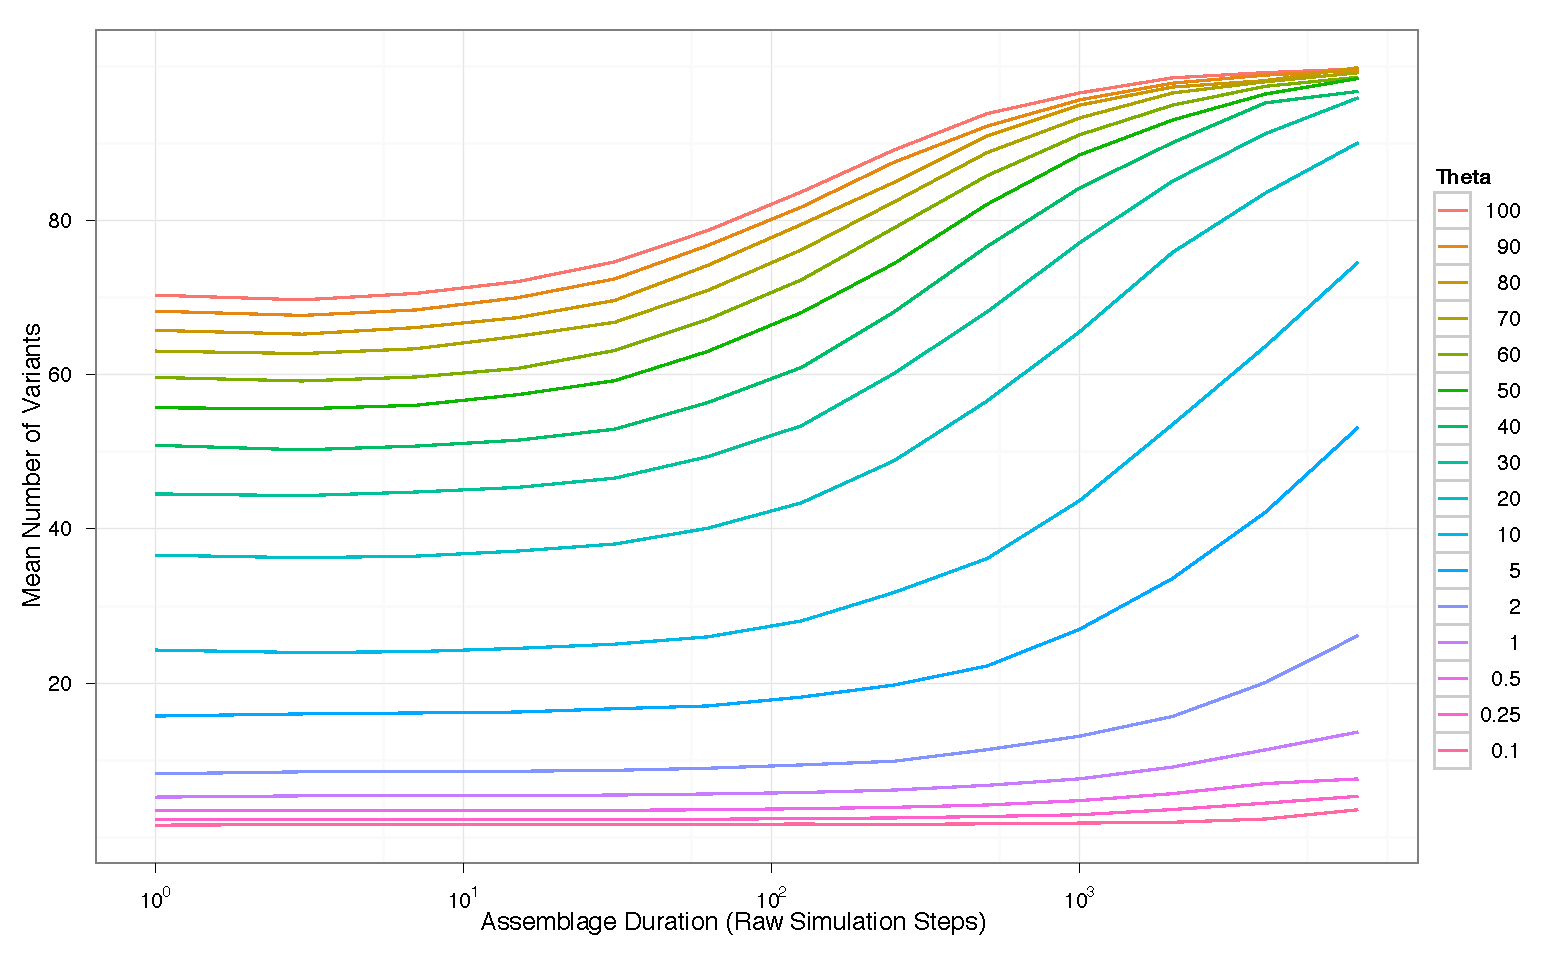
\includegraphics[angle=90, scale=0.75]{graphics/timeaveraging/unscaled_kn_by_duration_stacked.pdf}
	\caption{Mean value of $K_n$ for \timeavd samples, plotted against assemblage duration in simulation steps, for each level of $\theta$ in the study.  Note that the ``onset'' of \timeav effects (as measured by increased $K_n$), is quite gradual at low $\theta$, while high innovation rates display increased richness with very minor amounts of \timeav.}
	\label{fig:unscaled_kn}
\end{figure*}

\subsection{Neutrality Testing}
\label{sec:slatkin-ta-effects}

The Slatkin Exact test for neutrality, discussed in Section \ref{sec:neutrality-test}, determines the ``tail'' probability for a sample of size $n$, with observed number of traits $k$, to be derived from the Ewens Sampling Formula (Equation \ref{eq:conditional-esd}).  The test employed in this study is Slatkin's Monte Carlo version, which allows the use of larger sample sizes, using random selection to create unlabeled configurations from the ESD to compare against the observed values.  The resulting tail probability is converted into a standard hypothesis test by selecting an $\alpha$ value.  For purposes of this study, I considered the upper and lower 5\% of tail probabilities to indicate that a sample was probably not derived from a neutral transmission model, leading to $\alpha = 0.10$.  

Given this $\alpha$ level, we should expect roughly 5\% of the samples taken from a pure neutral copying process to fall into each of the the upper and lower tail regions, and thus for a Slatkin Exact test to reject the null hypothesis of neutrality.  Roughly 90\% of the samples we take from the neutral WF-IA process should fall between $0.05 < p < 0.95$ and thus lead to acceptance of the null hypothesis.  This experimental setup also implies the limited utility of performing a single neutrality test on a single sample of class counts or frequencies, as has been archaeological practice by necessity.  A single Slatkin exact test with $\mathbb{P}_e$ value of, say, 0.96, would constitute some, but relatively weak, evidence of non-neutrality.  Better practice would be taking many samples from a large assemblage or multiple collections and calculating independent Slatkin tests for each sample, and examining their distribution.  

If \timeav has no effect on the validity of the Slatkin Exact test employed against temporally aggregated samples, we would expect the fraction of samples in the two tails (upper and lower 5\% in this case) to equal 10\%.  Anything over 10\% would constitute evidence of extra Type I errors, since we know the samples to have been generated by a process meeting the definition of the null hypothesis.  Therefore, after post-processing the simulation output to produce Slatkin tests as described in Section \ref{sec-ta-method}, I tabulated the fraction of Slatkin Exact tail probabilities that exceeded the expected 10\% tail population.  These are, in other words, ``excess'' failures of the Slatkin Exact test, beyond those expected by the probability distribution itself.  For each $\theta$ level, and for each \timeav duration, the mean ``excess'' failure rate was computed, from the 1,113,134 raw Slatkin Exact test results generated in the simulation study.  

\begin{figure*}
%\centering
	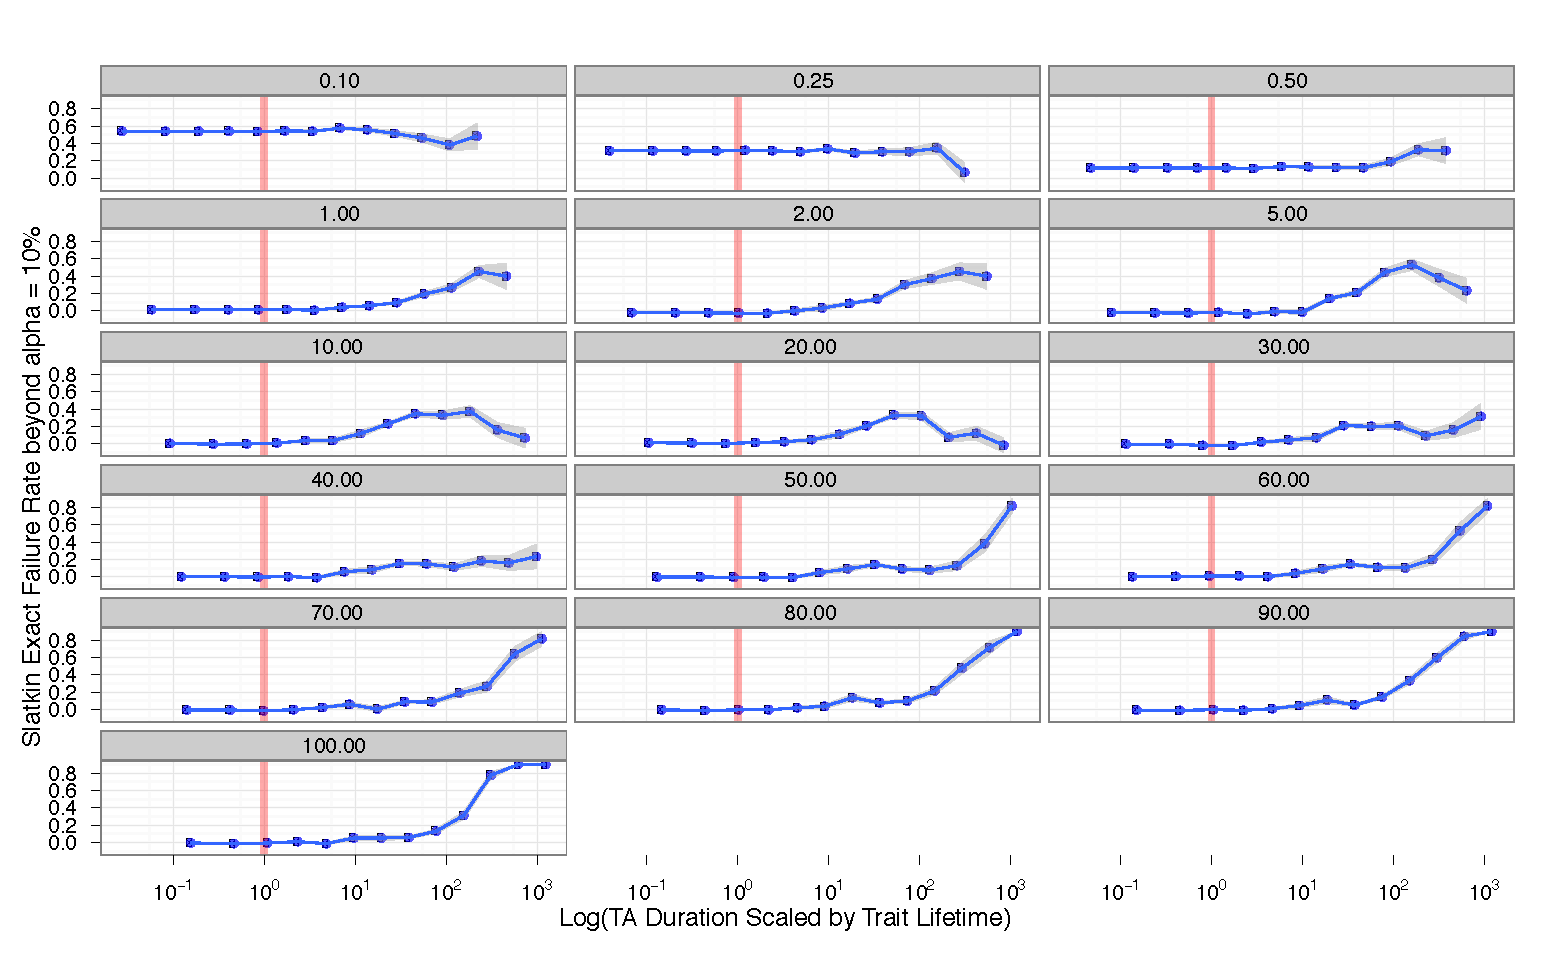
\includegraphics[angle=90, scale=0.75]{graphics/timeaveraging/slatkin-test-theta-0_1-100-100-5k-40k-failure-means-with-abline-labels.pdf}
	\caption{Slatkin Exact test failure rate (above the expected 10\% given two-tailed test with $\alpha = 0.10$, plotted against \timeav duration scaled by mean trait lifetime, for each level of $\theta$ in the simulation study. The red vertical line indicates the mean trait lifetime for that $\theta$ value, and the shaded region encompasses the standard error of the estimates for mean failure rates at each duration.}
	\label{fig:extra-slatkin-failures-by-scaled-duration}
\end{figure*}

Figure \ref{fig:extra-slatkin-failures-by-scaled-duration} depicts the relationship between the excess failure rate, and \timeav duration scaled by the mean trait lifetime (as previously described).  The mean trait lifetime is indicated by a vertical red bar in each graph.  Three major results are apparent.  First, at values of $\theta \geq 1.0$, the excess failure rate in non-time-averaged data is zero, as one would expect, and then begins to increase (albeit slowly) as the \timeav duration of samples exceeds the mean trait lifetime.  In some cases, such as $\theta = 5.0$, the Slatkin Exact test continues to be accurate given the chosen $\alpha$ value through samples which are aggregated for 10 times the mean trait lifetime.  But in all cases, with sufficient \timeav, the Slatkin Exact test begins to suffer from increased Type I error, reporting an ever increasing fraction of samples as not derived from a neutral transmission process.  The extreme situation is seen at very high rates of innovation, where nearly every test fails, at high levels of \timeav.  These failures are caused by saturation of a finite sample with singleton traits, causing the sample to display too much evenness in frequency to have been the result of sampling from the Ewens Sampling Formula.  But unrelated to this saturation effect, there is considerable failure in employing the Slatkin Exact test to detect neutrality.  For example, at $\theta = 5.0$, at 100 times the mean trait lifetime, approximately 70\% of all samples appear in the tail region of the distribution, compared to the expected 10\%.  Clearly, the Slatkin Exact test is not robust for long-duration assemblages.    

Second, at low $\theta$ values, the test results show excessive Type I error, even without \timeav.  There are several potential causes.  It is possible that the WF-IA process had not reached quasi-stationarity by 750 time steps, when sampling began.  This would mean that the effects of initial trait assignment might still be present and skewing the frequency distribution of traits.  Second, the Slatkin test is sensitive to the number of rare or singleton traits given the sample size, and in a small population (2000 individuals) with a low innovation rate (e.g., $\theta = 0.1$), counts of rare traits could be unstable.  This would not typically be the case in samples from large populations or entire species.  I do not consider the cause of this anomaly further in this paper, but it warrants further simulation study.   %Finally, at intermediate $\theta$ values (e.g., 10.0 - 30.0), the failure rate peaks at intermediate levels of \timeav, and then declines again).  This, too, is an unexplained effect warranting future research.

In general, with long-duration assemblages, archaeologists should be careful interpreting the results of neutrality tests adopted from population genetics.  The effect seen here can be summarized as:  with significant \timeav, trait frequencies generated by unbiased \ct can falsely appear to be non-neutral and thus driven by bias or selection (Type 1 error).  The longer the duration of an assemblage with respect to the mean trait lifetime, the larger the probability of a Type 1 error.  With sufficient duration, in fact, the probability of a Type 1 error becomes virtually certain, and the Slatkin Exact test loses any discriminatory power.  In summary, if one were to employ Slatkin's test to examine the hypothesis of neutrality in long-duration archaeological deposits, one would overwhelmingly come away with the impression that most \ct was biased, either towards conformity or a pro-novelty bias -- regardless of the underlying process occurring during prehistory.  

%It is worth noting that the effect appears to work in reverse when the data are known to be generated by a biased transmission process, such as conformist transmission.  Given the space constraints of a conference presentation, I leave the details of biased transmission models to another paper, but I performed a preliminary analysis of the conformist transmission model used by \citet{Mesoudi2009}.\footnote{Alex Mesoudi graciously provided the source code for simulations used in their paper, and I constructed a \tf module which replicated their exact algorithm for conformity.}  At even reasonably low levels of conformity (only a 10\% chance of a copying event being conformist rather than unbiased), Slatkin Exact tests upon unaveraged samples universally rejected the $H_o$ of neutrality -- virtually all samples concentrated themselves into the upper tail region.  At very high levels of \timeav, however, the null hypothesis began to be accepted, although at low frequency.  
%
%I conjecture that at low levels of conformist bias, and in relatively long duration assemblages, there can be equifinality between unbiased and conformist models, with respect to tests which fit trait counts to Equation \ref{eq:conditional-esd}.  This equifinality could be resolved, however, with a sufficient number of independent samples Slatkin Exact tests, since even a \timeavd unbiased process generates $\mathbb{P}(E)$ in both halves of the ESF distribution, whereas a pure conformist process under \timeav may generate $\mathbb{P}(E)$ values into the non-tail region of the ESF, but only from above, and not symmetrically around the center of mass of the ESF.  


%Clearly, we need to develop tests which can reliably distinguish neutral from biased transmission processes in the presence of significant \timeav.   Furthermore, when we compare results between assemblages, making an argument that some assemblages are more likely to be the result of (for example) conformist transmission, as opposed to unbiased transmission in other assemblages, the assemblage durations should either be approximately equal (with respect to the mean trait lifetime, which sets the timescale for such comparisons), or we need to consider the effect of the differential in durations when interpreting the test results.  

\subsection{Theta Estimation and Innovation Rates}
\label{sec:theta-estimation-results}

There would be considerable value in estimating the population-level innovation rate ($\theta$) from sample data if it could be done accurately.  As discussed in Section \ref{sec:theta-estimation-theory} above, such estimates are usually biased and have large variance.  In this section, I examine the effects of \timeav upon theta estimates generated from the samples taken to perform neutrality tests in the previous section.  For each of the 1.1 million samples of variants (distributed across actual theta values and assemblage durations), I calculated theta estimates given Watterson's approximation \citep{durrett2008}:

\begin{equation}
\label{eq:watterson-theta-est}
	\hat{\theta} \approx \frac{k_n}{log\;n}
\end{equation}

For each combination of actual theta and assemblage duration, theta estimates were averaged, to give a mean estimated theta value ($\mathbb{E}(\hat{\theta})$), and its standard deviation.  The results are shown in Table \ref{tab:estimated-theta-unaveraged}.   There are two regions of behavior apparent in the table, corresponding to drift- versus innovation-dominated dynamics.  At and below $\theta = 1.0$, estimated values are higher than the actual $\theta$ used to generate samples, and above 1.0, theta estimates begin to systematically lag below the actual theta value.  Overestimation at $\theta \leq 1.0$ matches the simulation results by \citet{ewens1974note}, although the authors did not simulate innovation rates above 2.0 (a large value in most genetic situations).  In addition to being biased, theta estimation appears to be even \emph{approximately} accurate only within a narrow range of values around $\theta = 1.0$.  

\begin{table}[ht]
\begin{tabular}{|c|c|c|}
  \hline
$\theta_0$ & $\mathbb{E}(\hat{\theta})$ & $\sigma(\hat{\theta})$ \\ 
  \hline
0.10 & 0.36 & 0.21 \\ 
  0.25 & 0.50 & 0.26 \\ 
  0.50 & 0.76 & 0.33 \\ 
  1.00 & 1.17 & 0.42 \\ 
  2.00 & 1.85 & 0.51 \\ 
  5.00 & 3.49 & 0.67 \\ 
  10.00 & 5.23 & 0.87 \\ 
  20.00 & 7.93 & 0.95 \\ 
  30.00 & 9.70 & 0.99 \\ 
  40.00 & 10.99 & 0.99 \\ 
  50.00 & 12.19 & 1.00 \\ 
  60.00 & 12.94 & 1.01 \\ 
  70.00 & 13.76 & 0.97 \\ 
  80.00 & 14.32 & 0.98 \\ 
  90.00 & 14.85 & 0.94 \\ 
  100.00 & 15.27 & 0.95 \\ 
   \hline
\end{tabular}
\caption{Mean Estimated Theta ($\mathbb{E}(\hat{\theta})$) from Samples (n=100) compared to actual values employed in simulation models ($\theta_0$), without any time-averaging.}
\label{tab:estimated-theta-unaveraged}
\end{table}

Figure \ref{fig:theta-estimates} examines estimates of theta by \timeav duration scaled by the mean trait lifetime, for each level of actual $\theta$ used in the simulation runs.  The pattern evident in synchronic or unaveraged samples carries over to \timeavd assemblages:  below $\theta \leq 1.0$, theta estimates are larger than the actual values, and increase in a non-linear fashion with assemblage duration.  Above 1.0 but below about 30.0, theta estimates begin below the actual value, cross the actual value, and continue to accumulate as assemblage duration increases.  Finally, at the very highest innovation rates, in a sample size 100, theta estimates are always drastic underestimates of the actual value, even with long assemblage duration increasing the accumulation of traits.  

\begin{figure*}
%\centering
	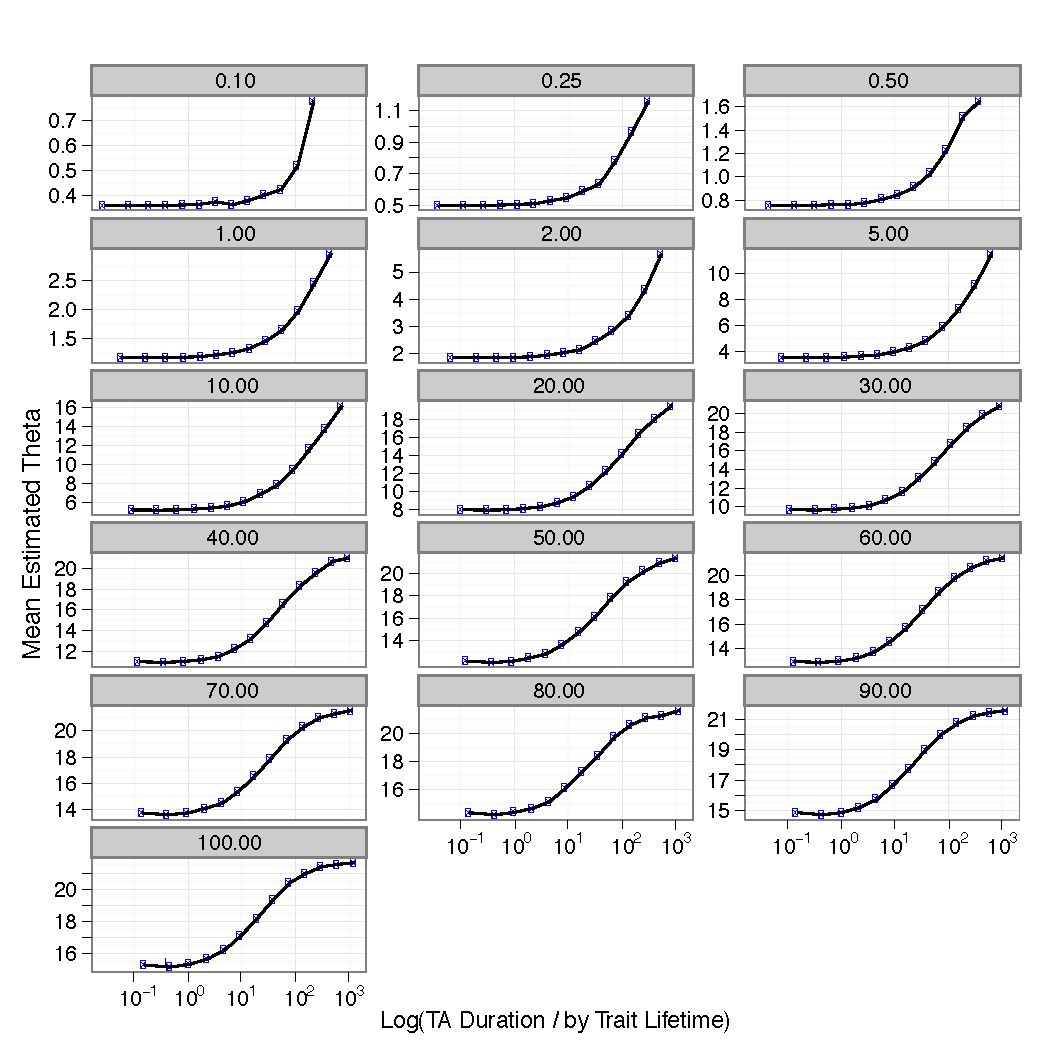
\includegraphics[scale=0.85]{graphics/timeaveraging/theta-estimates-scaled-MTL-theta-01-100.pdf}
	\caption{Estimates of mean population innovation rate ($\mathbb{E}(\hat{\theta})$) from samples ($n = 100$) taken for neutrality tests, using the approximation by \citet{watterson1975number}.  Plotted against assemblage duration, for each level of actual innovation rate used in simulation runs. }
	\label{fig:theta-estimates}
\end{figure*}

The Slatkin Exact test software also provides an estimate of $\theta$, finding the maximum likelihood value of theta when $K_n$ is set in Equation \ref{eq:expected-kn} to equal the observed value (this is the $t_e$ statistic introduced to archaeological usage in \citealp{Neiman1995}).  Figure \ref{fig:theta-estimates-slatkin} depicts the Slatkin theta estimates by \timeav duration scaled by the mean trait lifetime, for each level of actual $\theta$ used in the simulation runs.  One interesting difference between Figure \ref{fig:theta-estimates} and the Slatkin theta estimates is that the latter are more accurate for actual $\theta \geq 1.0$ than the Watterson approximation, in unaveraged assemblages.  Unfortunately, with increased assemblage duration, estimates explode to much larger values than those calculated by the Watterson approximation (i.e., $\theta \approx 1500$ for true $\theta = 30$ at maximum assemblage duration of 1000 times the mean trait lifetime, compared to the \emph{underestimate} of approximately 22 in Figure \ref{fig:theta-estimates}). 

\begin{figure*}
%\centering
	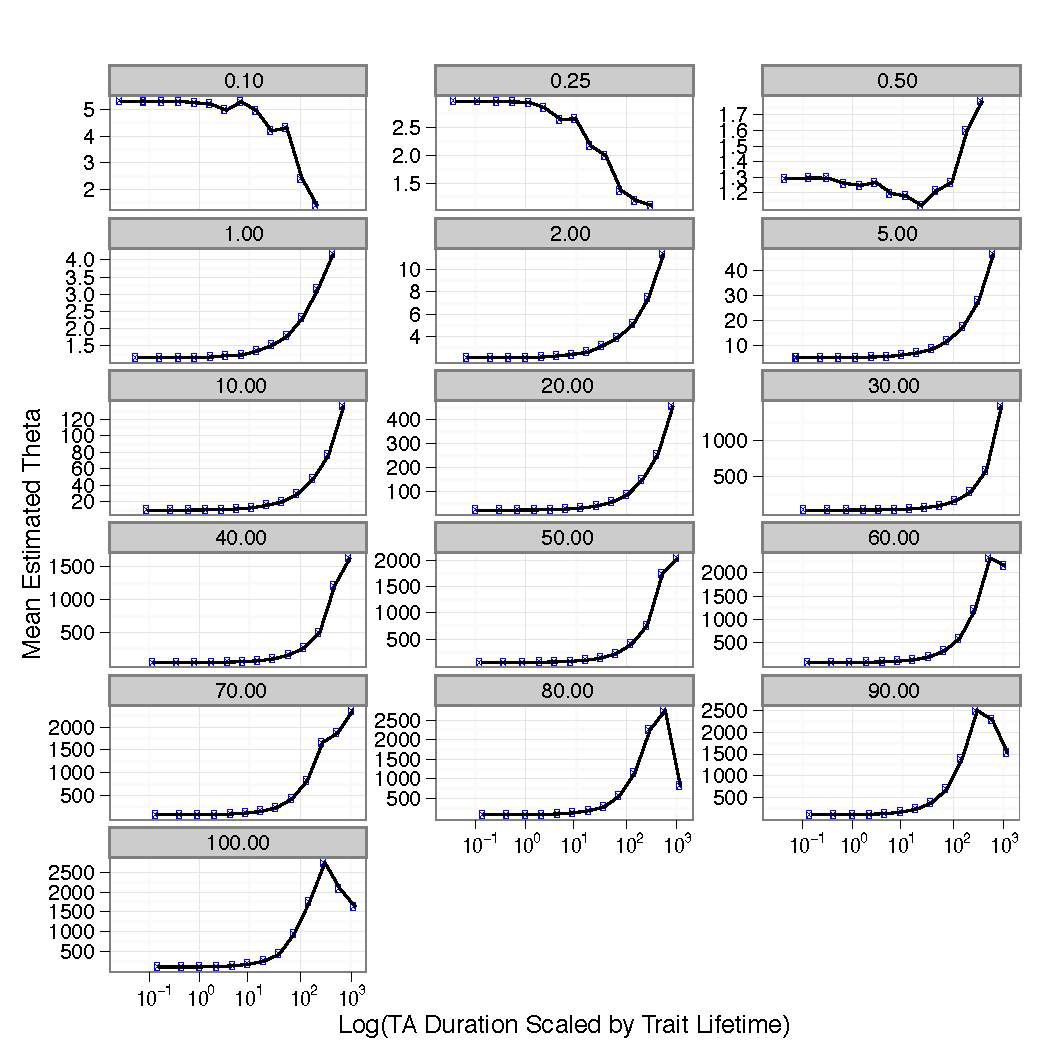
\includegraphics[scale=0.85]{graphics/timeaveraging/theta-estimates-scaled-Slatkin-theta-01-100.pdf}
	\caption{Estimates of mean population innovation rate ($\mathbb{E}(\hat{\theta})$) from samples ($n = 100$) taken for neutrality tests, using results from Montgomery Slatkin's neutrality test software.  Plotted against assemblage duration, for each level of actual innovation rate used in simulation runs. }
	\label{fig:theta-estimates-slatkin}
\end{figure*}

In short, estimation of population-level innovation rates from samples of artifacts using either estimation method are inaccurate, and the \timeav effect of accretional deposition renders such estimates even more inaccurate.  Clearly, such values cannot be used as actual indications of innovation rate or to ``work backward'' towards past population sizes.  And without fairly precise control over assemblage duration, the use of $t_e$ as a relative diversity measure between assemblages (in the manner common to archaeological applications) is highly suspect.  In the next section, I turn to $t_f$, the other common diversity measure in archaeological studies, which does not require an estimate of $\theta$, employing instead the variant frequencies directly.    

\subsection{Diversity Measures}

Much of the current effort in distinguishing biased and unbiased transmission models rely upon trait evenness and the shape of frequency distributions, given Alex Bentley's application of power-law distributions to both ancient and contemporary data sets \citep{Bentley2003,bentley2004random,Bentley2007,bentley2007fashion, bentley2009physical,8913,8914}.  One of the ways that unbiased and ``conformist'' models of \ct differ is in the expected amount of variation.  Compared to unbiased transmission, conformism of even a mild degree tends to strongly concentrate adoption onto a very small number of traits \citep{Mesoudi2009}.\footnote{This is especially the case when conformist transmission is implemented in simulations as a ``global'' rule where only the most common trait is copied during ``conformist'' copying events, rather than weighting all traits by their relative popularity.  Very little work has been done to compare the results from different methods of simulating biased transmission models.  This is a topic which would benefit greatly from additional research.}  It is difficult, however, to interpret the absolute number of traits ($K_n$) without knowledge of the population size, so \citet{8977} employed diversity measures instead in his classic examination of conformist transmission in Southwest pottery.  

\begin{figure*}
%\centering
	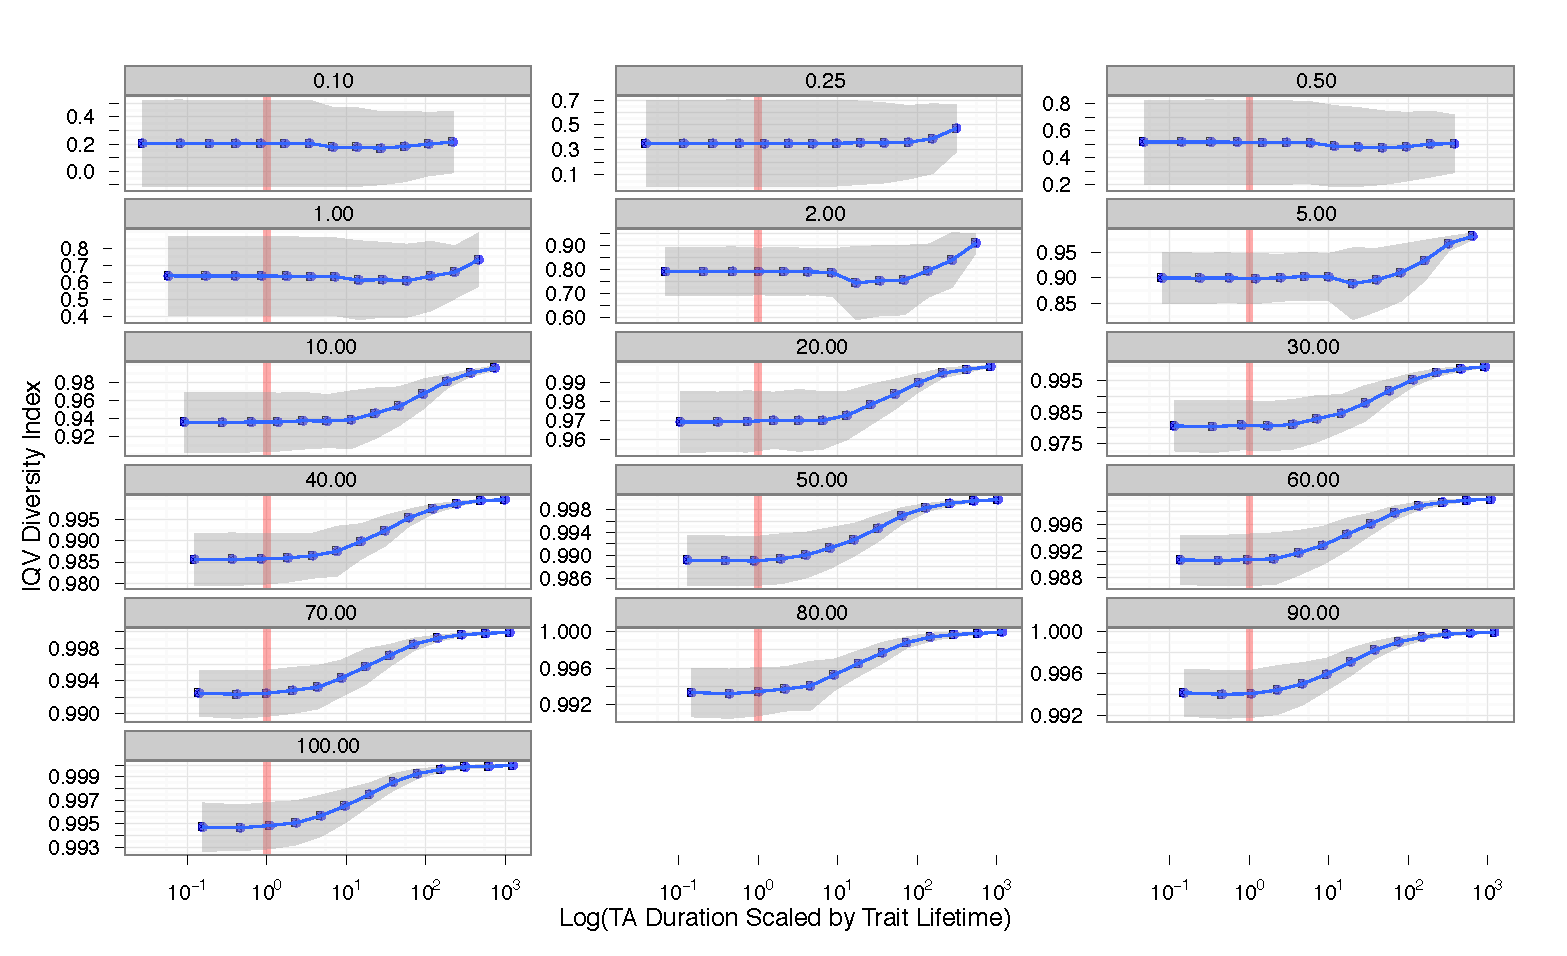
\includegraphics[angle=90, scale=0.75]{graphics/timeaveraging/wf-0_1-100-100-iqv-index-abline-labels.pdf}
	\caption{IQV diversity index, derived from samples of size 100, plotted against \timeav duration scaled by mean trait lifetime, for each level of $\theta$ in the simulation study. The red vertical line indicates the mean trait lifetime for that $\theta$ value.}
	\label{fig:iqv-est-by-scaled-duration}
\end{figure*}  

The most commonly used measure in the archaeological literature on \ct is $t_f$ (Equation \ref{eq:tf-formula}), since it is related to Wright's original measures of heterozygosity and thus associated directly with the historical development of the Wright-Fisher model.  But it is useful to normalize the results of $t_f$ between 0 and 1 so that we can compare different levels of theta and assemblage durations easily, in the same way that statisticians occasionally employ coefficients of variation or normalize covariances into correlation coefficients.  Equation \ref{eq:iqv-formula} does exactly this, and is called the ``index of qualitative variation'' (IQV) \citep{wilcox1973indices}.

Figure \ref{fig:iqv-est-by-scaled-duration} displays the relationship between the IQV for samples of size 100, and \timeav duration scaled by mean trait lifetime, as before.  IQV values range from 0.0, if only a single trait occurred within a sample (which happens in simulations with very low innovation rates), through 1.0, which indicates that traits are perfectly evenly distributed within a sample.  Even at the highest innovation rate studied, values of 1.0 were not seen in \emph{unaveraged} samples from the simulation runs.  It is apparent that \timeav can yield greater evenness among trait frequencies, although the plateau in IQV values  seen at high $\theta$ and high assemblage duration is a function of the saturation of $K_n$ in a finite sample seen above.  At very low innovation rates ($\theta \ll 1.0$), \timeav in contrast seems to have little effect on the dispersion of trait frequencies, with one or a very few traits always dominating a sample.



In between, when innovation rates are sufficient to guarantee at least one innovation on average per model generation ($\theta = 1.0$) but fewer than 10, there is non-monotonic behavior apparent in the IQV index.  For example, at $\theta = 2.0$, \timeav has no effect on IQV until duration is 10 times the mean trait lifetime (\mtl), at which point assemblages begin to appear \emph{less even} in frequency distribution, until about 100 times the mean trait lifetime, when evenness begins to steadily increase.   This effect is interesting, since it suggests that we cannot easily compare diversity indices between assemblages unless we control for duration or have independent evidence concerning innovation rates.   
 

\section{Discussion and Conclusions}
\label{sec:conclusions}

When we examine the effects of \timeav on the sample properties of unbiased transmission, using the mean lifetime of traits as our fundamental time scale, several lessons for practical applications emerge.  First, it appears that assemblages with very small amounts of temporal aggregation display little of the distributional alterations that characterize long-duration assemblages.  Statistical tests of neutrality and diversity measures, and thus arguments based on them, can probably be used with care.   Second, estimates of population-level innovation rate derived from Ewens's sampling formula are biased (and therefore inaccurate), and become seriously inaccurate with increased assemblage duration.  Archaeologists should strongly reconsider using $t_e$ or other theta estimates even in relative comparisons, and should definitely not consider such estimates to reflect the innovation rate or population size present in the prehistoric population.  Third, for assemblages that have a duration longer than the mean trait lifetime, it is important to measure and control for the relative duration of assemblages when comparing statistical results across samples.  Without doing so, we cannot interpret relative differences of diversity indices or trait richness values as indicative of different modes of transmission.  

One caveat to the above is that such effects refer specifically to \emph{assemblage} level data, composed of many artifacts deposited over time.  Artifact-scale analysis, where the attributes under analysis come together in a short period of time, and where single artifacts comprise the counting unit for transmission studies, will not necessarily suffer the quantitative effects described here, or would suffer no measurable \timeav effects if the assemblage durations were short compared to the lifetime of traits.  A good example of this is Jonathan Scholnick's chapter in the present issue, expanding on his previous research into \ct in Colonial America through gravestones \citep{premo2011spatial,scholnick2010apprenticeship}, where his samples cover 10 year periods based on the death dates carved on each stone.  

Furthermore, while the mean lifetime of transmitted information plays a central role in establishing a ``natural'' time scale over which \timeav affects  unbiased transmission, this time scale is not an archaeological one.  This discrepancy in time scales arises because the abstract ``traits'' of our models are not equivalent to the classification units employed by archaeologists.  This is not a trivial difference, and is one that is rarely even discussed in archaeological applications of \ct models.  Instead, we frequently act as if  ``traits equal types,'' despite occasional acknowledgement of the difference. 

But we have no direct empirical access to the information prehistoric populations were learning, teaching, and imitating.  We will never find ``units of transmission'' in any empirical sense for archaeological applications of \ct models, and we have no warrant to equate our models of prehistoric information flow with the classes we use to observe it today.  Long ago, \citet{8874} recognized that when anthropologists study the ideas held within a social group under study, what is actually being studied are the ideas we \emph{construct} about the ideas individuals in other cultures may have had.  \citet{Dunnell1971} systematized this distinction, pointing out that we always operate with analytic classes whose construction is done by archaeologists, for archaeological purposes.  These classes serve as a ``filter'' by which we detect patterns in artifact assemblages, which reflect patterns in the information which flowed within past populations.  There is no ``natural'' set of classes to employ in studying \ct, but we often forget to incorporate this fact into our analyses.  Linking the time scale over which variation entered and left a prehistoric population, and the time scale over which archaeological classes appear and then exit the archaeological record will involve further research on the relationship between transmission dynamics and complex, multi-dimensional archaeological classes.  Such research is essential to connect the abstract quantities described by theoretical models, to observable aspects of the archaeological record.  

These results paint a fairly gloomy picture of almost all of the standard variables archaeologists have used since Neiman's \citeyearpar{Neiman1995} pioneering work.  One wonders why empirical studies using diversity measures, innovation rate estimates, or neutrality tests appear to ``work'' and give sensible results?  One possibility, of course, is that some studies don't yield the expected results.  We see this, possibly, in a fascinating analysis by \citet{steele2010ceramic}.  The authors employed ceramic classes that appeared to be non-neutral and subject to selection or biased transmission.  Yet Slatkin exact tests were unable to rule out the null hypothesis of neutrality.  I do not present an analysis of conformist transmission under \timeav in this article, but using \tf I see evidence that temporal aggregation has the opposite effect on Slatkin exact tests in populations with weak conformist biases:  neutrality tests suffer increased Type II error, making it more likely that we will accept a null hypothesis of neutrality when the opposite is the case.  

Another possibility is that certain variables may retain their distributional character, but have their values inflated by temporal aggregation.  In such situations, there would be no reason to reject the neutral model, but inferences about the values of parameters would be inaccurate.  Even if investigators did not rely upon the absolute value of parameters, frequently such inferences (e.g., diversity values) are employed as relative comparisons between assemblages.   I suspect that this has occurred in a number of published studies, but few \ct applications include detailed information concerning assemblage duration, so it is difficult to redo the researcher's original hypothesis tests with temporal controls, without going back to original field information or reports.  Clearly, both possibilities may also occur in some situations.  

As archaeological usage of \ct theory becomes more frequent and we move from proof-of-concept studies to demanding interpretive accuracy from our models, methodological research is essential to ensure that our applications are empirically and dynamically sufficient.  The present study focused on a necessary first step in such method development, developing an understanding of the effect of \timeav in accretional assemblages upon the observable variables in neutral \ct models.  The results demonstrate that frequently employed statistics, such as $t_e$, are highly inaccurate and biased when measured in \timeavd assemblages, and that neutrality tests are subject to enough additional Type I or Type II error that the results can be systematically misleading.  Clearly, in order to apply \ct models to diachronic data derived from \timeavd assemblages, we need to develop observational tools and methods suited specifically to the archaeological record, instead of simply borrowing statistical methods and models from theoretical population biology.  



\section{Acknowledgements}
This paper was originally presented in a symposium titled \emph{``Recent Developments in Cultural Transmission Theory and its Applications''} at the 2012 Annual Meeting of the Society for American Archaeology, Memphis, TN.  The author wishes to thank Kristen Safi, the organizer, for the opportunity to participate, and Carl P. Lipo, Fraser Neiman, James Feathers, Jonathan Scholnick, and Michael J. O'Brien for comments on drafts of this paper. 







\chapter{Can We Identify Biased Cultural Transmission in the Archaeological Record?}
\label{chap:ctmixtures-paper}

\section{Introduction}\label{ctmixtures:sec:introduction}

The emerging field of cultural evolution is the study of cultural change in humans and other animals as a Darwinian evolutionary process, and encompasses research in biology and the social sciences.  As part of an ``extended synthesis’’ \citep{Pigliucci2010}, cultural evolution extends  the notion of ``descent with modification’’ to include the learning and accumulation of cultural information between generations, and explicit study of the differences in structure and pattern between genetic and cultural transmission.  Beginning with the seminal work by Cavalli-Sforza and Feldman 
\citeyearpar{CF1981} and later by Boyd and Richerson \citeyearpar{BR1985}, the study of these differences has focused a great deal of attention on cognitive and psychological biases that create population structure.  Over the past thirty years experiments, observational studies, and theoretical models have come together to create a picture of human social learning which is biased towards conformity under many circumstances and the observation of success, positive payoffs, and social prestige as a basis for selecting those from whom one learns or imitates \citeeg{richerson2005not}.  

Most of the evidence for this emerging picture of human social learning comes from controlled experiments and observational studies of living populations.  Most of it is conducted by psychologists and anthropologists \citep{whiten2016cultural,mesoudi2016evolution}.  Archaeologists and paleoanthropologists seeking to study the evolutionary history of social learning are consumers of this body of theory.  There is nothing wrong with being a consumer of evolutionary theory---every discipline involved in applying Darwinian insights to human social behavior is a consumer in some area---but we must also be producers of methods needed apply that theory to the unique empirical phenomena we study.  Our job consists, at a high level, of building methods for constructing models appropriate to the kinds of data we possess, understanding how to best to assess the fit between those models and our data, and finally, understanding the limits of our ability to do so given the nature of the empirical phenomena we study.  

This paper addresses the limits of our ability to select among detailed, individual-level models of cultural transmission in most archaeological situations.  Initial optimism applying mathematical models of cultural transmission to archaeological data \citeeg{Neiman1995,eerkens2005cultural,Lipo1997,Shennan2001ceramic,Jordan2003} has given way to a more nuanced view of our ability to discriminate between models \citep{barrett2019equifinality,premo2010equifinality,kandler2019analysing}.  A growing body of work is aimed at assessing the causes of equifinality between cultural transmission models given archaeological data, for example assessing the effects of time averaging \citep{Madsen2012,Porvcic2014,Premo2014,perreault2018time} and non-stationary population sizes \citep{Rorabaugh2014,kandler2018generative}.  The hope is that methodological development will help us understand, and correct for, these sources of equifinality so that we can proceed with ``model selection'' and fitting (albeit in a more sophisticated way) and still work with the kinds of transmission models that other anthropologists and social psychologists employ (especially those derived from Boyd and Richerson's seminal work on ``dual inheritance theory'').  

There is no question that we can empirically detect different types of social learning modalities in controlled experiments \citep{kempe2014experimental,mesoudi2006bias,whiten2016cultural,mesoudi2008cultural,Mesoudi2008a,Mesoudi2014}.  Experiments and detailed observational studies of living populations generate fine-grained data about who individuals learn from and what covariates affect ``chains'' of transmission.  Archaeologists, even in the best of circumstances, always face data which is coarse-grained compared to  that available in experimental settings.  To one degree or another, the data we generate from archaeological deposits are estimates of some population-level prevalence of cultural traits.  

Understanding the limitations of using coarse grained data to perform model selection is crucial for archaeology and paleoanthropology,   The main approach to identifying the best fit cultural transmission model for a data set has been to construct univariate statistical tests or distributional expectations for various summary statistics.  Examples of summary statistics employed in this model fitting approach include richness or diversity (evenness) measures, the average amount of time traits survive in a population, their turnover properties, or the degree to which frequency data match distributions known to arise in various “null” models \citep{Shennan2001ceramic,shennan2008style,Bentley2003,shennan2008style,Kandler2013,Kandler20150905}.  These statistics are highly attractive for archaeological purposes because most are easy to calculate from standard descriptions of archaeological assemblages without additional measurements on individual artifacts and thus allow the study of previously described data sets.  

This approach has now been employed in enough studies, and with enough replications on the now-paradigmatic ceramic data from the European Neolithic Merzbach Valley, that we can evaluate its performance.  Kandler \citeyearpar{Kandler20150905} notes that after five separate analyses of the Merzbach data using a variety of summary statistics and approaches, the results remain in conflict.  It is not clear whether the data are consistent with a hypothesis of neutrality, or anti-conformity/novelty seeking, or whether both are reflected in different assemblages.  

There has been much less focus on the crucial question of whether some of the equifinality we face is simply structural.  By ``structural'' equifinality, I mean that the models we expect to be able to identify cannot be distinguished because they overlap too strongly in their outcomes, with any possible data we can obtain.  This paper is an attempt to outline a major cause of structural equifinality in cultural transmission modeling:  the inherent variability of social learning modes within real populations.  The simulation experiments reported here seek to understand whether individual variability in cultural transmission and social learning strategies renders our models impossible to distinguish given coarse grained data, and what effects that sampling and time averaging have on our ability to distinguish the true data generating process behind our data.

This study employs simulation from several data generating models, and employ multiple summary statistics and a powerful machine learning classifier capable of finding highly nonlinear decision boundaries to determine whether it is even possible to discriminate between our theoretical models.  If we can, then it is reasonable to expect that further methodological research on ways to ``correct'' or avoid sources of equifinality may be fruitful.  If we cannot distinguish between models, even in the idealized case, then I believe we must question the utility of attempting to perform the kind of microevolutionary model fitting that many of us have been attempting with archaeological data.  

The results indicate that populations with mixtures of bias can be distinguished from a reference population of unbiased copiers very accurately given a full population census and the absence of time averaging.  In this sense, equifinality between these theoretical models may not be structural even with coarse-grained data.  However, the introduction of sparse sampling and the interaction of sampling with time averaging markedly degrades our ability to accurately classify samples as to their model of origin.  Furthermore, the pattern of errors is not symmetric.  With sampled, time averaged data, we are extremely likely to conclude that samples represent various kinds of transmission bias, even when this is not the case.  

This result deepens the skepticism we should feel as archaeologists about the ability to apply detailed social psychological models to most archaeological data.   Instead of attempting to adapt our data so that we can apply microevolutionary models, we may be better off adapting our models to the data and empirical record we actually possess.  This means looking at coarser grained models and coarser grained research questions which may better match the unique strengths of a diachronic, aggregated record of human evolution.  

\section{Within Population Variation in Social Learning:  A Cause of Structural Equifinality?}\label{ctmixtures:sec:structural-equifinality}

The microevolutionary models of cultural transmission we typically employ in archaeology draw structurally upon the mathematical core of classical population genetics, but add inheritance structures and social learning modes informed by observations across the social sciences \citep{CF1981,BR1985}.  The core models in dual inheritance theory richly vary in the cognitive biases they describe, but all still tend to ignore significant sources of population structure or variation.  All tend to assume \emph{panmixia} as a simplifying assumption, and most tend to depict the population-level consequences of sets of individuals who employ a single learning mode or class of cultural ``parent'' to learn from \citep{wimsatt2019articulating}.   

Real populations, as opposed to those depicted in much of our modeling, have rich structure.  Human populations are mixtures of people of different ages, genders, and propensities for individual versus social learning.  There also appears to be variation among populations and major cultural lineages in these mixtures of social learning traits.  Detailed experimental and observational studies are just beginning to document this variation \citep{whiten2016cultural,yaveroglu2002cultural,tweed2002learning,chang2011cultural,enquist2007critical,csibra2009natural,tomasello2016ontogeny,lopez2010attention,berl2015cultural,mesoudi2015higher,mesoudi2016evolution}  People can vary in these propensities over the course of their lifetimes \citep{lehmann2013optimal,demps2012social,correa2009children,mesoudi2016evolution}, making demographic factors important in modeling the population-level effects of individual social learning processes.    

Even if different ways of learning from parents and peers are distinguishable from individual level data, we should not automatically assume that their population level consequences are distinguishable, when there is variation in the population.  Processes which are distinguishable with transmission chains, for example, may have opposing effects on population-level summary statistics.  A population comprised of conformists who prefer to learn and stick with the ways that have worked in the past would tend to display fewer variants in the population than expected in a neutral equilibrium, and more concentration of frequency on a small number of traits.  A population comprised of those who prize novelty and exploration of ``new'' traits will tend to display more variants than expected, with more evenness among trait frequencies.  A real population that combines individuals with both propensities 
would display a mixture of these population-level consequences.  In other words, some of the effects easily visible at the individual level may ``cancel out''.  If that is the case, can we distinguish a mixture of these social learning biases, from a population of unbiased copiers?  

\begin{figure}[ht!]
  \centering
  \includegraphics[scale=0.5]{graphics/ctmixtures/equifinality-transmission-bias-scenarios.pdf}
  \caption{Two scenarios for how equifinality may affect our ability to empirically distinguish between different models of cultural transmission given the effects of sampling and time averaging.}
  \label{ctmixtures:fig:equifinality-scenarios}
  \end{figure}

This question becomes even more concerning when we combine the “structural” possibility of equifinality just described with the “methodological” sources of equifinality previously discussed:  sampling and the time averaging characteristic of aggregated, time transgressive data.  This question is depicted schematically in Figure \ref{ctmixtures:fig:equifinality-scenarios}.  In the left panel, under mild to moderate amounts of time averaging and with reasonable sample fractions, our ability to discriminate between models may be relatively strong, with equifinality restricted to situations with small sample size and in assemblages with significant duration.  The right hand panel depicts the other end of a continuum of possibilities:  our ability to identify transmission models given data might be quite rare across a range of values relevant to archaeological inquiry.  This paper is an attempt to determine where we might stand between these two poles.  Given even simplified models of mixed social learning processes, can we tell apart their population level consequences, especially with limited samples and in the presence of time averaging?

\section{Methods}\label{ctmixtures:sec:methods}

\subsection{Study Design}\label{ctmixtures:sec:study-design}

I approach this question by simulating populations with mixtures of social learning or transmission biases.  In particular, I examine populations comprised of mixtures of conformist and anti-conformist individuals, along with a ``reference'' population of unbiased copiers \citep{BR1985}.  The simulated populations are censused at sampling intervals and trait counts recorded.  This allows us to later perform a variety of ``data collection regimes'' which simulate the effects of archaeological sampling and the time averaging effects of aggregate deposition in the archaeological record.  It also allows analysis at the single trait level, or the composition of traits into ``classes'' which simulate the effects of archaeological classification, since most efforts to fit cultural transmission models to real data have accepted existing classification schemes as input to the model fitting.  

The output of the simulation runs are simulated archaeological observations of trait or class frequency count at a variety of levels of sample size and time averaging ``treatments'' from the same underlying data generating processes.  This allows us to examine our ability to distinguish between data generating processes depending upon the ``treatment'' levels, given a method for predicting which data generating process produced the data points observed.  In the next section, I describe a predictive modeling approach, adopted from machine learning, for measuring equifinality as error in properly predicting the known data generating process for our simulated data.  

\subsection{Measuring Equifinality Through Classification Error}
\label{sec:equifinality-classification-error}

The common models of cultural transmission employed by archaeologists are stochastic in nature, and thus when we take samples from simulations of those models, we will observe a distribution of results for any summary statistic we choose to observe.   To the degree that several models generate separable distributions for the chosen summary statistics, we will be able to infer the most probable data generating model given values of those statistics.  If the distributions of summary statistics have some overlap, the level of certainty with which we can predict the correct data generating model will decline overall, and perhaps be no better than chance in the region of overlap.  

This generic situation is shown schematically in Fig.
\ref{ctmixtures:fig:distributional-scenarios}. Here, three pairs of probability models
are represented by 500 measurements each of two continuous predictors variables (e.g., a diversity index).
In the left panel, the pair of models do not overlap in their outcomes.
Given a data point, we can assign it to Model 1 or Model 2 with
virtually no error, and thus we would consider models 1 and 2 to be
distinct and not equifinal at all. The situation in the middle and right
panels of Figure \ref{ctmixtures:fig:distributional-scenarios} is different. There is
some overlap in the middle panel, and very strong overlap in the right
panel. In the right hand panel, in fact, there is enough overlap that on
average, our ability to assign a randomly chosen data point to the
correct model is no better than chance. Intuitively, we would say that
there is some equifinality in the middle panel, and that the two models
in the right hand panel were strongly equifinal.

\begin{figure}[ht]
\centering
\includegraphics[scale=0.6]{graphics/ctmixtures/distributional-overlap.pdf}
\caption{Simple example of model outcomes with different degrees of distinguishability given two summary statistics: (A) simulated data points from two fully separate models, (B) two models with a limited overlap region, (C) and two models whose outcomes are highly overlapping.}
\label{ctmixtures:fig:distributional-scenarios}
\end{figure}

Measuring the overlap between the measured outcomes of theoretical models thus provides a way to determine their inherent or structural equifinality given a set of observable summary statistics or observational variables.  When theoretical models are simple enough to have solvable equations, it may be possible to perform an analysis of distributional overlap using mathemetical tools such as the Kullback-Leibler divergence between their resulting probability distributions \citep{burnham2002model}.  In the kind of cases discussed in this paper, with mixtures of social learning modes in a single simulated population, we need a numerical and thus statistical approach.  We will operationalize measurement of distributional overlap by producing samples from each theoretical model, calculating or other producing the observable variables or summary statistics, applying any simulated data collection treatments (such as specific sampling regimes), and then attempting to ``predict'' which data generating model generated each data point.  The error rate in predicting the correct model is a quantitative measure of \emph{how much equifinality} there is between models, given a set of predictor variables and data collection treatments.  

In more formal terms, we define measurement of equifinality as the error in performing a classification task, in the machine learning sense \citep{murphy2012machine}.  Given a set
of models \(\mathcal{M}_1 \ldots \mathcal{M}_n\), we can measure
equifinality as the minimum possible error achievable in correctly
assigning simulated data points to the data generating model which produced them,
given measurement of a set of predictor variables or ``summary statistics.'' In the classification task, we ask which model has the highest probability for
a given data point, given the conditional density of the data and
models. This sounds exactly like Bayes' theorem, and in fact we can
write the classification problem as follows, where
\(Y \in 1, \ldots, K\) refers to each of \(k\) models, and
\(X_1, \ldots, X_p\) refer to \(p\) different predictor variables.

\begin{equation}
\mathbb{P}(Y | X_1, \ldots, X_p) = \frac{\mathbb{P}(Y_i) \mathbb{P}(X_1, \ldots, X_p | Y)}{\mathbb{P}(X_1, \ldots, X_p)}
\label{eq:bayes-rule-classification}
\end{equation}

\(\mathbb{P}(Y)\) plays the role of the prior distribution, and reflects how prevalent we expect each label or model to be in the population.  In a true empirical study this might be uniform---if we had no reason to suspect that a model may be more likely than another \emph{a priori}, or we may have substantive reasons for weighting models.  For example, models may capture the prevalence of a genetic factor, and we may have quantitative evidence for that prevalence.  In a theoretical study such as this one, we are simulating equal numbers of samples from each theoretical model, and thus the term will be constant and cancel out.  The data points in a classification problem are given, and
thus the denominator is also a constant. The most probable class for a given
data point reduces, therefore, to the mode of the likelihood function:

\begin{equation}
Y_{pred} = \argmax_y \mathbb{P}(X_1, \ldots, X_p | Y)
\label{eq:map-class-bayes}
\end{equation}

This is the \emph{Bayes classifier} for a controlled simulation
experiment, and its error rate in separating data points by model is
called the \emph{Bayes error}. This is the lowest possible error in
separating the models given the data
\citep{devijver1982pattern, fukunaga1990introduction, hastie2009elements}.
The Bayes error is zero when we can correctly identify each data point
as to its model of origin (as in the left panel of Fig. \ref{ctmixtures:fig:distributional-scenarios}, and rises as two models overlap in the
measurement space. With sufficient overlap, the Bayes error could
approach 0.5, which represents a prediction rule which is no better than
chance, or conceivably rise even further, indicating that our classifier performs even worse than coin-flipping.\footnote{Error rates can obviously be higher than 50\% in an empirical study, but in a controlled simulation study like the present paper, error higher than a coin-flip is indicative of a problem with the experimental setup.}

Unfortunately, we can almost never directly calculate the Bayes error
rate for a prediction or classification rule, because we rarely have an
expression for the likelihood function of our transmission models in the
spaced formed by the predictor variables. Bayes error can be directly calculated, in fact, only for
a small number of cases, such as Gaussian distributions with a shared
covariance
matrix.  There is a large literature, especially in pattern recognition and language classification, on approximating upper bounds for the Bayes error of a classifier, because it is highly useful to know when you cannot improve a recognition system or classifier any further \citep{Antos:1999dn, Dobbin:2009du, McLachlan:1975eo}.  Most such upper bounds are based upon parametric models, and use estimates of a distance metric between the classes being distinguished (typically, the Mahalanobis or Bhattacharyya distance) \citep{devijver1982pattern}.  Such bounds are difficult to apply in situations where we have complex social learning models, whose probability density functions in the space of measured variables are typically unknown.  

Despite the fact that we can rarely calculate the Bayes error rate, it
is useful as an operational definition for equifinality, since it
measures our uncertainty about model choice given a set of measurable
variables. In practice, we approximate the Bayes error by employing classifier algorithms which are able represent complex relationships between all of the predictor variables in order to get as close to the Bayes error rate as possible.  This generally means using methods with higher model ``capacity'' than the linear models familiar to most archaeologists (such as logistic regression or linear discriminant analysis).  Formally we seek methods with high Vapnik-Chervonenkis (or VC) dimension, which measures the ability to represent complex decision boundaries between classes \citep{vapnik2013nature}.  At present, methods such as boosting, bagging, and ensemble approaches that combine weaker methods such as decision trees with boosting combine high capacity with very low error across many benchmark cases \citep{hastie2009elements}, and thus come closest to estimating the
Bayes rate \citep{tumer2003bayes}.  

\subsection{Simulation Modeling of Cultural Transmission Mixtures}\label{ctmixtures:sec:ct-mixture-modeling}

In order to measure the overlap between various theoretical mixtures of social learning strategies, I built simulation models for the scenarios given in Table \ref{ctmixtures:tab:models}.  The outcomes of all four transmission models are derived by simulating the
dynamics of the model in an agent-based framework that allows each agent to be assigned a different transmission rule.  All simulations employ
the Moran dynamics, where one individual engages in a copying event at
each elemental step
\citep{moran1962statistical, moran1958random, aoki2011rates}.
Innovations are modeled using the ``infinite alleles'' approximation,
where every innovation is new to the population \citep{Ewens2004}.
Simulations were performed using the CTMixtures software package,
available as open source
software.\footnote{\url{https://github.com/mmadsen/ctmixtures}} The
parameters for all simulation runs are given in Table
\ref{tab:parameters}. Where there is a range given (e.g., innovation
rate), the parameter is treated as a prior distribution and each
simulation run is assigned a uniform random value from the range. This
ensures good coverage of the parameter space given 25,000 replicates for
each of the 4
models.\footnote{The use of a good prior distribution for parameter ranges also results in simulation data that are usable for later data fitting by approximate Bayesian inference \citep{Beaumont2010, Crema2014, Csillery:2010jd, Marin2012}.}

\begin{table}[ht]
    \begin{tabular}{ll}
        \hline
        Model Code & Model Description \\ 
        \hline
        Unbiased & Population with only unbiased copiers \\
        Equal Mixture & Equal numbers of conformists and anti-conformists \\
        Conformist Dom & 70\% conformists with 30\% anti-conformists  \\
        AntiConf Dom & 70\% anti-conformists with 30\% conformists \\
        \hline
    \end{tabular}
    \caption{Theoretical models that were simulated as part of this study.}
    \label{ctmixtures:tab:models}
\end{table}



\begin{table}[htb]
\begin{tabular}{lc}
\hline
Parameter & Value or Interval \\ 
\hline
Innovation rate (in $\theta$ scaled units)  & $[0.1, 5.0]$   \\
Probability of conformism & $[0.05, 0.25]$ \\
Probability of anti-conformism & $[0.05, 0.25]$ \\
Sample fractions & 0.1 and 0.2 \\
Time averaging intervals (units of 100 individuals) & 10, 20, 50, 100 \\
Population size & 100 \\
Number of trait dimensions (loci) & 4 \\
Initial traits per dimension & 10 \\
\hline
\end{tabular}

\caption{Parameters for simulation runs across the four models studied.  Intervals are treated as prior distributions, and each simulation run is assigned values derived from a uniform random sample on the interval indicated.  Lists of values are all applied to every simulation run (e.g., there is both a 10\% and a 20\% sample from each simulation run.  Single values are applied to every simulation run, and represent a point prior.)}
\label{tab:parameters}
\end{table}

Simulated populations are 100 individuals in size, because most
archaeological studies of cultural transmission have focused upon
situations where population sizes are assumed to be small. 
Each simulated individual carries 4 different
traits at any time, which are treated as separate loci or dimensions.  Trait frequencies are tracked on a per-locus basis, and combinations of loci are tracked in order to simulate archaeological ``types'' or classes which include multiple dimensions of variation.

Regardless of transmission model, social learning involves no interaction effects between loci in this study. The
population is seeded with 10 randomly chosen traits at each locus as a
starting configuration. The evolution of each simulated population proceeds
for 4 million elemental steps, which is equivalent to about 40,000
copying events on average per individual. This value was chosen by
performing simulations at 1 million time step intervals and verifying
that the distribution of a key statistic (the number of traits per Loci)
had stabilized. This occurred in most cases between 2 and 3 million
steps, and in all cases between 3 and 4 million, so the last value
was chosen.\footnote{The analysis underpinning this decision is available in the Github repository at \url{https://github.com/mmadsen/experiment-ctmixtures/analysis/verification}.}
At the end of 4 million simulation steps, a suite of variables are
measured from each of the 25,000 replicates and stored for analysis.


\subsection{Summary Statistic Selection}\label{ctmixtures:sec:variable-selection}

Since most previous work on identifying transmission mode from archaeological data employ single diagnostic variables, and begin to display equifinality under realistic data collection conditions, it is reasonable to examine whether using multiple variables will yield more discriminatory power in the same contexts.  By representing the outcomes of transmission models in a higher dimensional space, it should be easier to find a decision boundary (``separating hyperplane'') that correctly predicts the model which generated each data point, if such a boundary exists.  

\begin{table}[ht]
\begin{tabular}{ll}
\hline
Variable                                    & Model Variable \\ 
\hline
Cross-Tabulated Class Richness  (Class)         &  num\_trait\_configurations      \\
Slatkin Exact (Class)           & configuration\_slatkin       \\
Shannon Entropy (Class)  &  config\_entropy \\
IQV Diversity (Class)  & config\_iqv \\
Neiman $T_f$ (Class) & config\_neiman\_tf \\
Slatkin Exact (Max for Locus)                    & slatkin\_locus\_max       \\
Slatkin Exact (Min for Locus)                     & slatkin\_locus\_min      \\
Slatkin Exact (Mean for Locus)                   & slatkin\_locus\_mean       \\
Shannon Entropy of Trait Frequencies (Min)      & entropy\_locus\_max       \\
Shannon Entropy of Trait Frequencies (Max)       & entropy\_locus\_min      \\
Shannon Entropy of Trait Frequencies (Mean)      & entropy\_locus\_mean      \\
IQV Diversity Index (Min)     & iqv\_locus\_max \\
IQV Diversity Index (Max)     & iqv\_locus\_min \\
IQV Diversity Index (Mean)    & iqv\_locus\_mean \\
Trait Richness (Min)   & richness\_locus\_max \\ 
Trait Richness (Max)   & richness\_locus\_min \\
Trait Richness (Mean)    & richness\_locus\_mean \\
Kandler-Shennan Trait Survival (Min)   & kandler\_locus\_max \\
Kandler-Shennan Trait Survival (Max)   & kandler\_locus\_min \\
Kandler-Shennan Trait Survival (Mean)   & kandler\_locus\_mean \\
Neiman $T_f$ (Min)   & neiman\_tf\_locus\_max \\
Neiman $T_f$ (Max)   & neiman\_tf\_locus\_min \\
Neiman $T_f$ (Mean)   & neiman\_tf\_locus\_mean \\
\hline

\end{tabular}

\caption{Variables measured from each transmission model simulation sample.  The parenthetical expression records whether the variable was calculated for cross-tabulations of all 4 loci (Class) or represent the order statistics from individual loci (Min/Mean/Max).  The right column records the variable name used within R statistical models, for examining the relative importance of each variable in classifying observations.}
\label{tab:variables}
\end{table}

The predictor variables chosen in this study focus upon measures of richness and
diversity, trait survival over time \citep{Kandler2013}, and the
Slatkin neutrality test \citep{slatkin1996correction, slatkin1994exact}.
Each has been employed in the archaeological literature on identifying
cultural transmission modes, or is a variant on such measures (e.g., IQV
is a normalized version of Shannon entropy), and crucially, all are measurable in standard archaeological contexts using attribute or class frequency data.  This additionally makes most of the variables applicable to the re-analysis of already published data, which is an important usage scenario in archaeological research.   

For the locus-centric variables, each statistic was applied to each
locus separately, and the mean, minimum, and maximum of the values
obtained for each locus were recorded. I collect order statistics
in addition to the mean value, since it is possible that minima and
maxima might be a better discriminator between models than averages. In
addition to the variables calculated upon each of the 4 loci, the traits
at each locus were combined into a cross-tabulation of "classes" which simulates the
process of archaeological classification. Each class represents a
different combination of traits from the 4 loci, and very roughly
simulates observing cultural variation through the lens of a standard
paradigmatic classification \citep{Dunnell1971}. The same variables are
then measured as a function of the class counts.\footnote{The sole exception is the Kandler-Shennan survival time, which is not measured here for the cross-tabulated classes.  Understanding the quantitative behavior of this measure for multidimensional classes of traits is an important open research question, however.} This allows us to
understand whether transmission models are better distinguished on a
per-locus (dimension) basis or by operating on more complex classes that
combine several traits together. The full list of measured variables is
given in Table \ref{tab:variables}.

As a final note on variable selection, in an exploratory analysis for this
project, I tried to include the power law exponent as a summary statistic, given the important work by Bentley and colleagues
\citeyearpar{bentley2004random} and Mesoudi and Lycett
\citeyearpar{Mesoudi2009}.  Proper fitting of power law distributions to empirical data is more difficult than simply determining if a straight line describes the data after double logarithmic transformation; in particular testing if a data set displays a power law is difficult if there are a small number of counts and small sample size \citep{clauset2007power}.  This may be difficult in many archaeological cases where the number of classes may be relatively small (on the order of ten rather than hundreds), and the total sample sizes can be relatively small.  In their study, Mesoudi and Lycett
\citeyearpar{Mesoudi2009} use the cumulative number of adoptions of each
trait over the entire time span of their simulations as the ``frequency''
used to calculate power law
exponents.\footnote{I confirmed this by inspection of the source code for their simulation model, which was provided by Alex Mesoudi.}  This quantity is available in simulation but would unobservable in empirical data.  Whether or not to include power law exponents as predictor variables will depend strongly on the data set in question.  Given the experimental setup used in this study, power law exponents were difficult to calculate in a stable way.  Thus, I did not include them in the remainder of this study, and their discriminatory power in combination with other variables thus remains an open question.

\subsection{Data Collection Treatments}\label{data-collection-treatments}

At the end of each simulation run, after the model has reached a quasi-stable equilibrium (measured as stability in per-locus trait richness), a series of samples are taken from the evolving population.  These samples are taken in ways that correspond to various real-world data collection strategies.  First, a census of the entire population is taken.  This functions as a baseline for the ``most complete'' information we can use to identify transmission modes, and there are also conditions during observational studies or in laboratory experiments where census is possible.  In archaeological studies, anything approximating a census is usually impossible, although Jonathan Scholnick's study of New England gravestones and their makers may approximate this quality of data collection \citep{scholnick2012spatial}.  Second, the simulated population is sampled, at the 10\% and 20\% levels.  Sampled data is ubiquitous in archaeological research, and although the issues involved in mapping artifact samples to their meaning for the underlying population of social learners is complex and unresolved, it is useful to determine whether the overall sample fraction has a measurable effect upon model equifinality.  

Archaeology derives its empirical data by sampling a sedimentary record of artifact discard and trace fossil creation by many individuals, often over large spans of time \citep{schiffer1983toward,Schiffer1987,stein2001review,Stein1987,Stein1993,stein2001review,stein2003big}.  Thus, our data almost never represent synchronic or ``point in time'' samples of the results of human activity \citep{Grayson1998,lyman2003influence,Madsen2012,Porvcic2014,Premo2014}.  Therefore, the simulated samples of cultural transmission in this study are also temporally aggregated over a number of time steps, and the aggregate trait counts used to determine the frequencies of cultural traits over the entire interval.  The population census has no temporal aggregation, and thus does represent a synchronic census.  

Time averaging is implemented according to the schematic in Fig. \ref{ctmixtures:fig:kandler-sampling}.  At the end of the simulation run, sampling begins at a time index calculated to allow time averaged samples to be taken twice, with a gap of 50 ``generations'' to also allow the calculation of the Kandler-Shennan trait survival statistic (although unlike their original study, the values at the start and end times are inherently time averaged in this study, which would be the case in any real archaeological context) \citep{Kandler2013}.

\begin{figure}[p!]
\centering\includegraphics[scale=0.4]{graphics/ctmixtures/time-averaging-with-kandler-sampling.pdf}
\caption{Schematic of how trait survival as described by Kandler and Shennan \citep{Kandler2013} is extended to time averaged samples of transmission events.  Time runs from the start of the simulation run at the top, to the end at the bottom.  The interval of time over which we calculate the Kandler-Shennan trait survival is given as a simulation parameter, and represents the gap in the middle of the diagram.  Before and after that gap are sampling windows during which transmission events are accumulated over some number of simulated ``generations'' (values of 10, 25, 50, and 100 are used in this paper).  Trait survival is then calculated as the number of traits present in the starting time averaged sample of transmission events, which are still present in the ending time averaged sample of events.}
\label{ctmixtures:fig:kandler-sampling}
\end{figure}


\begin{table}[ht]
    \begin{tabular}{ll}
        \hline
        Sampling Strategy & Time Averaging Duration \\ 
        \hline
        Population Census & 0 \\
        10\% Sample & 10 \\
        10\% Sample & 25  \\
        10\% Sample & 50 \\
        10\% Sample & 100 \\
        20\% Sample & 10  \\
        20\% Sample & 25 \\
        20\% Sample & 50 \\
        20\% Sample & 100 \\
        \hline
    \end{tabular}
    \caption{Data collection strategies, applied to every simulation run.  Time averaging duration is given in units of "generations," which are units of 100 time steps (given the population size).  100 generations thus represents 10,000 elemental time steps in the Moran simulation dynamics.}
    \label{ctmixtures:tab:measurement-strategies}
\end{table}

The data collection strategies employed in this study are given in Table \ref{ctmixtures:tab:measurement-strategies}.  Applied to all 23 variables, the study yielded approximately 900,000 samples from the four transmission models listed in Table \ref{ctmixtures:tab:models}.\footnote{All data and analyses for this study are available as part of a Github repository, although large data files are kept on Amazon S3 for long-term storage.  See \url{https://github.com/mmadsen/experiment-ctmixtures} for details.  The published analysis described here is the ``equifinality-4'' data set.}  

\subsection{Classifier Selection and
Training}\label{classifier-selection-and-training}

Classifier algorithms are supervising learning models from statistics
and machine learning that predict a categorical response from a mixture
of discrete or continuous variables \citep{hastie2009elements}. The most
familiar classifiers in archaeological practice are logistic regression
and discriminant function analysis, but neither is competitive with
contemporary ``ensemble'' methods which combine many classifier rules
into a single prediction. In such models, combining predictors can both
reduce the variance of prediction (e.g., bagging added to traditional
classifiers and random forests), and
reduce bias.  Some classifiers, like boosted trees, can do both.

Since the Bayes error rate of comparing two complex transmission models is not something we can calculate or even estimate, we must approximate it using the best performing classifier model available.  A very general result in statistical
decision theory (called, appropriately, the ``No Free Lunch'' theorems)
guarantee that there is no single prediction model that can achieve the
best result with every data set and problem
\citep{wolpert2002supervised, wolpert1997no}. Thus, I took a compromise approach, selecting several algorithms that are known to have excellent performance across a range of data sets, and then performing a pilot study using the four transmission models previously described.  A recent study
compared 179 classifier algorithms on 121 different data sets
(representing the entire UC Irvine Machine Learning Database), and found
that random forests \citep{breiman2001random}, support vector machines,
and gradient boosted classifiers performed the best
\citep{hastie2009elements}. Additionally, some ensemble methods (random
forests and gradient boosted classifiers) provide information on
variable importance as an integral part of the algorithm.  Since understanding which of our 23 variables are useful for separating transmission models is an important aspect of this study, I evaluated random forests against gradient boosted classification trees using small simulated samples from each transmission model.\footnote{The data for this initial comparison are available in the \url{https://github.com/mmadsen/experiment-ctmixtures} repository under the experiment name ``equifinality-2''.}
Gradient boosted models outperformed random forests on these simulated
data, are comparable in computational costs, and are used for all
further results in this paper.

Gradient boosted classification operates by repeatedly fitting a set of
decision trees to the data \citep{AlexeyNatekin2013,hastie2009elements}. In each round, decision trees are fit to the training data, and individual data points scored as errors or successful predictions.  Subsequent trees are fitted by modifying the trees in the direction that minimizes the residual error.  This is equivalent to finding the gradient of the loss function in the space of possible classifier functions, hence the name of the method.  The impact of each gradient step is smoothed by including a ``shrinkage'' factor.  Finally, the gradient steps are ``boosted'' to weight data points by the success in prediction, such that data points that are frequently misclassified become targeted by the algorithm until they can be correctly predicted \citep{freund1995boosting, freund1999short, schapire2012boosting}.  After a specified number of iterations, the class or label membership of each data point is obtained by having each gradient step classifier tree ``vote'' for class membership, and the final answer is the majority vote.  This class of models can also be visualized as repeated refitting of residuals until error is minimized \citep{friedman2001greedy}.  This combination of boosting and iterative function search is very powerful, and gradient boosted models regularly achieve top accuracy in benchmark studies.

In this study, I employ the R package (\textbf{gbm}) for gradient
boosted classification \citep{ridgeway1999state}, with the binomial deviance \(\textrm{log}(1 + \textrm{exp}(-2y\hat{y}))\) as our loss function, where \(y\) is the true
model for a data point, and \(\hat{y}\) is the classifier model's
prediction.  Binomial deviance approximates the ``zero-one'' loss function with one which is differentiable, which is needed for a gradient descent method.  The tuning parameters for this study (number of boosting iterations, depth of classification trees) were selected using 5 rounds of repeated 10-fold cross-validation on the training data \citep{Kim:2009im, kuhn2013applied}.

The full data set of simulation samples, after data collection treatments, was split into two chunks. 80\% of the data were
used to train the classifier model, and 20\% were held back to provide an
unbiased evaluation of classifier performance.  For each comparison of models
reported, the training data were thus fitted 50 times across
different values of the tuning parameters (number of boosting
iterations, and depth of decision trees), and the best performing
parameters chosen from the repeated cross-validation sets. The final model is then constructed using the entire
training set and the optimal parameter values. All classifier tuning,
final model fitting, and test error evaluation was performed using Max
Kuhn's superb \textbf{caret} package for R
\citep{kuhn2008building, kuhn2013applied}.  The final results reported are those achieved on the 20\% of data points held out for evaluation.


\subsection{Classification Error and Equifinality
Assessment}\label{classification-error-and-equifinality-assessment}


The basic data for assessing the quality of a classifier model is the
\emph{confusion matrix}, which compares classification successes and
errors for a data set.  A hypothetical example is given in Table
\ref{tab:confusion-matrix}.  The most basic measure of classification quality is the \emph{accuracy}, or the ratio
of correct predictions to the total number of data points.  In the confusion matrix, this is the ratio of the sum of diagonal elements to the sum of off-diagonal elements.  In the example given in Table \ref{tab:confusion-matrix}, the classifier is 82.5\% accurate. We often also use the misclassification rate, which is simply $1 - \emph{accuracy}$.  

\begin{table}[ht]
\begin{tabular}{c|cc}
 & Actual Model: & \\
 Predicted &  Model 1 & Model  2 \\
  \hline
 Model  1 & \textbf{9000} & 2500 \\
   Model  2 & 1000 & \textbf{7500} \\
\end{tabular}
    \caption{Example confusion matrix.  Columns correspond to the actual model for data points, rows correspond to predictions from a classification model.  Bold numbers on the diagonal correspond to correct predictions, the off diagonal elements correspond to classification errors.}
    \label{tab:confusion-matrix}
\end{table}


When the classes
being predicted are not balanced, and especially if there are a small
number of one class compared to another, a better statistic is Cohen's
``kappa'' \citep{kuhn2013applied}, which compares observed accuracy to
what one would expect purely from chance, given the marginal totals:

\begin{equation}
\kappa = \frac{O - E}{1 - E}
\label{eq:kappa}
\end{equation}

where \(O\) is the observed accuracy, and \(E\) is the expected accuracy
due to chance given the ratio of classes in the marginal totals of the
confusion matrix. Kappa ranges from \(-1\) to \(+1\), with \(0\)
indicating no agreement between predictions and the real class
memberships. High values indicate good agreement, while values below
\(0.5\) and especially less than \(0.2\) indicate very poor predictive
ability \citep{altman1991practical}. In the present context, a
classifier comparison (for example, biased versus neutral models with no
sampling or time averaging) that yield a high kappa value are strong
evidence that no equifinality exists between the two situations, since
the classifier is highly accurate. Low kappa values are evidence that
despite strong statistical methods and many variables to choose from, we
cannot distinguish between models, and thus the models may be equifinal.  

\section{Results}\label{ctmixtures:sec:results}

From the four models listed in Table \ref{ctmixtures:tab:models}, I examine three comparisons.  The first comparison addresses our general capability to distinguished unbiased (or neutral) cultural transmission from samples drawn from populations with mixtures of both conformist and anti-conformist propensities.  The second examines our ability to distinguish between an unbiased population, and a population comprised of a majority of conformists, with 30\% anti-conformists, to create a mixture of social learning modes.  The third compares an unbiased population with a majority of anti-conformists, with 30\% conformists, to produce the opposite configuration.

\begin{figure}[p!]
\centering\includegraphics[scale=0.65]{graphics/ctmixtures/eq5-kappa-dotchart-full-predictors.pdf}
\caption{Cohen's kappa values for model comparisons, using a classifier trained on all predictors including per-locus and ``classes'' built from intersecting loci and then counting frequencies.  Top panel provides results for comparing a neutral, unbiased population and a balanced mixture of conformist and anti-conformists.  The middle panel provides results for unbiased compared to a population dominated by anti-conformists.  The bottom panel depicts results for unbiased compared toa population dominated by conformists.  Each panel presents results for the 9 data collection treatments analyzed.}
\label{ctmixtures:fig:kappa-full-predictors}
\end{figure}

\begin{figure}[p!]
\centering\includegraphics[scale=0.65]{graphics/ctmixtures/eq5-kappa-dotchart-perlocus-predictors.pdf}
\caption{Cohen's kappa values for model comparisons, using a classifier trained only on predictor variables derived from per-locus trait counts.  Top panel provides results for comparing a neutral, unbiased population and a balanced mixture of conformist and anti-conformists.  The middle panel provides results for unbiased compared to a population dominated by anti-conformists.  The bottom panel depicts results for unbiased compared toa population dominated by conformists.  Each panel presents results for the 9 data collection treatments analyzed.}
\label{ctmixtures:fig:kappa-perlocus-predictors}
\end{figure}

For each of the three comparisons, the Cohen's kappa scores were calculated two ways:  with all predictive variables (including the class variables measured on intersections of attributes from the 4 different loci), and for classifiers built only with per-locus variables (i.e., where we look only at what would be single attributes rather than more complex archaeological classes or culture-historical types.  

\subsection{Classification Error and Equifinality Results}

In this section I outline the results from the three model comparisons described above, across all 9 data collection treatments.  Figure \ref{ctmixtures:fig:kappa-full-predictors} depicts Cohen's kappa results for the classifier trained with all predictor variables, including those from per-locus trait counts, and those from intersecting all four loci into ``classes'' that mimic the way paradigmatic classifications are constructed to build archaeological types \citep{Dunnell1971}.  Figure \ref{ctmixtures:fig:kappa-perlocus-predictors} provides the Cohen's kappa results for the classifier trained only on predictor values derived from per-locus trait counts.  

What is strongly apparent, however, is population-level, coarse grained data \emph{can} reliably distinguish between a population of unbiased copiers and various mixtures of individuals with differing propensities for conformism and anti-conformism.  Using multiple variables in a classifier model creates sufficient discriminatory power that we can distinguish these models reliably, even in a balanced mixture with equal numbers of conformists and anti-conformists.  The effects do not, apparently, ``cancel out.''  

This ability to distinguish models, however, is only apparent where we can census the entire population (or, presumably take very large samples), and where there is no time averaging.  We should, in other words, expect to be able to identify pure and mixed models of social learning modes in situations where we can obtain synchronic samples, and capture enough of the population that we can accurately capture all of the variation present.  This is possible in experimental contexts, and in many contemporary data sets that represent data on whole populations.  That's good news for researchers seeking to use microevolutionary models to study social psychological phenomena related to social learning in contemporary contexts.

Even more strongly apparent, however, is that accuracy rapidly declines as sample fraction decreases and as time averaging increases.   As one might expect, larger samples offer more accurate predictions than smaller samples.  Within the larger, 20\% sample, when cross-tabulated class and per-locus predictors are included, accuracy is highest with the smallest amount of time averaging (10 generations), and decreases as time averaging increases.  When we remove cross-tabulated class predictors, and simply look at per-locus variables, this clean pattern is not apparent, and accuracy is not a function of time averaging duration.  Furthermore, for the smaller 10\% sample with all variables included, accuracy is not a function of time averaging duration.  In these cases, Cohen's kappa values are between 0.2 and 0.3, indicative of a very poor classification model with very little predictive power. 

While sample size is partially addressable in data collection, the degree to which archaeological deposits are aggregated over some window of time is often not alterable in research design.  There is equifinality here which we simply cannot avoid in most archaeological cases, which renders our ability to distinguish between realistic mixtures of social learning modes and unbiased copying unreliable at best, and impossible at worst.  

\subsection{Which Predictor Variables Help Discriminate Models?}

% \begin{table}[ht]
% \begin{tabular}{rc}
%   \hline
% Importance & Predictor Variable \\
%   \hline
% 100.00 & Cross-Tabulated Class Richness \\
%   50.71 & Slatkin Exact for Classes \\
%   29.50 & Shannon Entropy (Mean for Locus) \\
%   23.13 & Shannon Entropy for Classes \\
%   19.66 & IQV Diversity (Mean for Locus) \\
%   11.58 & Kandler-Shennan Trait Survival (Mean for Locus) \\
%   \hline
% \end{tabular}
% \caption{Relative importance of predictor variables for population census data, in the comparison between unbiased transmission and all biased models.  The most important variable is (by convention) scaled to 100, and the values indicate the ratio of variable importance to the variable which is most effective at classifying data points.  Only values greater than 10 are shown. The remainder of the predictor variables are 1/100th as effective as class richness or less.}
% \label{ctmixtures:tab:varimp-popcensus}
% \end{table}

Since there is some predictive power here, particularly using population census information, it is important to understand which variables were providing that discriminatory power.  
Gradient boosting algorithms allow measurement of how much each predictor variable contributes to a classification model.  The importance of a variable is assessed over the iterations of tree construction by estimating the relative improvement in training set misclassification error from adding the variable to the model.  The importance values are usually scaled such that the most important variable has a score of 100, and variables with smaller importance values are less important to classification power.  

In general the pattern is the same across comparisons, so I illustrate variable importance by examining the comparison between unbiased copiers, and the population composed of a balanced mixture of conformists and anti-conformists.  Table \ref{ctmixtures:tab:varimp-balbiased-census} gives the relative importance of predictor variables when the classifier includes classes created by intersecting the 4 loci with individual traits.

Most classificatory power in this comparison comes from the richness in the cross-tabulated classes.  In general, richness (whether class or per-locus) dominated all of the classifier models, which is not surprising given the central role of the amount of variation in mathematical treatments of the Wright-Fisher and Moran models \citep{Ewens2004}.  The second variable in importance in this comparison is the p-value for a Slatkin's ``exact'' test, which determines the probability that a given set of class frequencies come from the Ewens Sampling Distribution \citep{slatkin1994exact}.  The Shannon entropy, a measure of evenness in frequency (in this case averaged across loci) provides about half as much predictive power as richness. Interestingly the Kandler-Shennan survival time, averaged across the 4 loci, offers significant discriminatory power, suggesting that the method used here for simulating it along with time averaging is a fruitful avenue for additional research.  Beyond this, the predictors have increasingly little power, likely because we have multiple variants on evenness measures in the full list of summary statistics, and their results are collinear with other variables. 

\begin{table}[ht]
\begin{tabular}{rc}
  \hline
Importance & Predictor Variable \\
  \hline
100.00 & Cross-Tabulated Class Richness \\
  85.49 & Slatkin Exact for Classes \\
  47.12 & Shannon Entropy (Mean for Locus) \\
  24.12 & Kandler-Shennan Trait Survival (Mean for Locus) \\
  18.88 & IQV Diversity (Mean for Locus) \\
  10.85 & Shannon Entropy for Classes \\   
  \hline
\end{tabular}
\caption{Relative importance of predictor variables for population census data, in the comparison between unbiased transmission and a balanced mixture of pro- and anti-conformists.  The most important variable is (by convention) scaled to 100, and the values indicate the ratio of variable importance to the variable which is most effective at classifying data points. Only values greater than 10 are shown. The remainder of the predictor variables are 1/100th as effective as class richness or less.}
\label{ctmixtures:tab:varimp-balbiased-census}
\end{table}

\subsection{Time Averaging Makes Identification of Bias More Likely}

As shown in these results and previous studies \citep{Madsen2012,Porvcic2014,Premo2014}, the temporal aggregation we encounter in archaeological data is a significant barrier to discriminating between theoretical models of cultural transmission.  Equifinality increases as the amount of time averaging represented in a data set increases.  But this is not the whole story.  Time averaging, combined with sampling effects, do not simply make our classifiers worse in a random manner.  Instead, there is substantial bias in the pattern of classification (and thus model identification) errors.  

We can see this clearly by examining two confusion matrices from the comparison between unbiased and a balanced mixture of social learning biases.  Table \ref{ctmixtures:tab:confusion-matrix-census} shows the pattern of correct and incorrect predictions for the population census with no time averaging treatment.  In the confusion matrix, the rows depict the \emph{predicted} data generating model, and the columns provide the true data generating model.  Thus, in the row ``biased'', the first column are correct predictions that data points came from the mixture of biases model, while the second column are incorrect predictions that the data points arose from a model of bias, when the data points in fact arose from unbiased copying.

Even in the population census treatment, there is a slight tendency for prediction errors to be unbalanced.  It is more likely to misidentify a data point arising from unbiased copying as coming from a mixture of biased copiers than it is to make the opposite error.  In other words, we over-identify bias, even with complete data, by about 30%.  

Table \ref{ctmixtures:tab:confusion-matrix-sampledata} shows the pattern of errors for the same comparison, but with 20\% sample fraction and time averaging duration of 50 steps.  This is not the worst treatment for accuracy by far, but note that the pattern of errors has become significantly more asymmetric.  With this data collection treatment 2.7 times more likely that we will make an error favoring an identification as transmission bias than that we will misidentify bias as neutrality.  

\begin{table}[p!]
	
    \begin{tabular}{|c|c|c|}
      \hline
     & biased & neutral \\ 
      \hline
    biased & 14898 & 132 \\ 
      neutral & 102 & 4868 \\ 
       \hline
    \end{tabular}
    \caption{Confusion matrix for comparison of unbiased versus mixed bias models, for the data treatment with population census of trait frequencies and no time averaging.}
    \label{ctmixtures:tab:confusion-matrix-census}
\end{table}

\begin{table}[p!]

    %`Sample Size:  20  Duration:  50`
    \begin{tabular}{|c|c|c|}
      \hline
     & biased & neutral \\ 
      \hline
    biased & 13926 & 2724 \\ 
      neutral & 1074 & 2276 \\ 
       \hline
    \end{tabular}
    \caption{Confusion matrix for comparison of unbiased versus mixed bias models, for the data treatment with 20\% sampling fraction and 50 steps for time averaging duration.}
    \label{ctmixtures:tab:confusion-matrix-sampledata}
\end{table}

By looking at the ratio of the right column in each confusion matrix, across all data collection treatments, we can see how the magnitude of this asymmetric preference for identification of bias scales with sample size and duration of time averaging  (Table \ref{ctmixtures:tab:misclassification-neutral}).  The smaller our samples are from the original population, and the more temporal aggregation in our assemblages, the more likely we are to ``see'' biased cultural transmission, even with combinations of summary statistics and powerful classifier models.

\begin{table}[ht]

\begin{tabular}{|l|c|}
  \hline
Data Collection Treatment & \% of Unbiased Data Points Misclassified as Biased \\
  \hline
Population Census & 2.6 \\
  Per-Locus Population Census & 3.4 \\
  Sample Size:  20  Duration:  10 & 49.1 \\
  Sample Size:  20  Duration:  25 & 49.5 \\
  Per-Locus Sample Size:  20  Duration:  25 & 49.7 \\
  Per-Locus Sample Size:  20  Duration:  10 & 50.1 \\
  Per-Locus Sample Size:  20  Duration:  50 & 54.4 \\
  Sample Size:  20  Duration:  50 & 54.5 \\
  Sample Size:  20  Duration:  100 & 57.6 \\
  Per-Locus Sample Size:  20  Duration:  100 & 58.1 \\
  All Sample Sizes and TA Durations & 68.0 \\
  Per-Locus Sample Size:  10  Duration:  25 & 73.5 \\
  Sample Size:  10  Duration:  25 & 73.6 \\
  Sample Size:  10  Duration:  50 & 73.7 \\
  Per-Locus Sample Size:  10  Duration:  10 & 73.8 \\
  Per-Locus Sample Size:  10  Duration:  100 & 74.0 \\
  Per-Locus Sample Size:  10  Duration:  50 & 74.1 \\
  Sample Size:  10  Duration:  100 & 74.4 \\
  Sample Size:  10  Duration:  10 & 74.7 \\
   \hline
\end{tabular}

    \caption{Percentage of data points from the unbiased transmission model that are falsely identified as arising from a biased model.}
    \label{ctmixtures:tab:misclassification-neutral}
\end{table}


\section{Discussion}\label{ctmixtures:sec:conclusion}

The central aim in this study has been to examine whether realistic mixtures of social learning strategies present fundamental equifinalities that were impossible to distinguish using population level summary data.  The results demonstrate that mixtures of biased social learning strategies do not ``cancel out'' sufficiently to mask their statistical signatures---when you have enough data, synchronic observations, and use several summary statistics in combination.  

However, when time averaging is present, and especially with small sample sizes, our ability to discriminate between theoretical models essentially disappears.  Equifinality is omnipresent.  Even worse, the results indicate that our ability to distinguish between models does not degrade symmetrically.  In the presence of time averaging and with small samples, we are several times more likely to identify data points as arising from transmission bias than we are when we have synchronic and more complete data.  

Archaeologists engaged in the study of microevolutionary cultural transmission models should employ a healthy skepticism about the enterprise of fitting artifact class frequency data to models.  Even with diachronic methods such as trait survival \citep{Kandler2013}, multiple summary statistics, and powerful analytic methods, there is little evidence that we can distinguish these models with simulated data.  And that should give us great pause in thinking that our conclusions from analyzing archaeological samples are sound.  It is time to evaluate whether the application of microevolutionary models in archaeology is a fruitful enterprise, or whether our time is better spent deriving models which are robust in the face of time averaging---even if those models address larger scale questions instead of the social psychological questions involved in most dual inheritance theory.  

It is certainly true that evolutionary change is ultimately caused by individual variation and how that variation affects success.   In a sense, all evolutionary change is ``caused'' by that individual level variation; patterns and processes we observe at larger spatiotemporal scales and taxonomic levels are ``upper level effects'' of individual level variation \citep{walsh2019paradox}.  This does not make population, regional, and taxonomic level patterning in evolutionary history mere ``epiphenomena.''  Far from it.  The structure and history of populations and their environments provide the fitness landscapes which shape and sort variation among individuals.  Archaeology is uniquely placed not just to document variation at larger scales, but to study processes that are only operative at scales larger than individuals and single populations.

We do not have a complete catalog of evolutionary processes that can only be studied above the level of single populations, but there are numerous examples. Variation in traits which affect dispersal lead to phenotypic variation among populations depending upon their migration and dispersal characteristics, an effect that \citet{shine2011evolutionary} refer to as ``spatial sorting.''  We can and should expect such differences to be evidence at archaeological scales when we compare sedentary versus mobile communities in the archaeological record, for example.  Niche construction often occurs over evolutionary time \citep{Laland2000,Odling-Smee2003,Odling-Smee2007}, including all kinds of coevolutionary relationships such as domestication \citep{rindos1984origins}.  All of these processes require the time depth inherent in the archaeological record for proper study and explanation.  Large scale population structure---patterns in interaction between communities, is something we can document at mesoscopic and macroevolutionary scales, and is part of what we mean when we discuss ``social complexity.''  Building models for these kinds of processes requires tools for creating diachronic models and fitting them to coarse grained, time averaged data.  In the following chapters, I turn to several methods for creating such models and evaluating equifinality among them.  




\chapter{Combinatorial Structure of the Deterministic Seriation Method with Multiple Subset Solutions}
\label{chap:seriationcombinatorics-paper}

\begin{description}[leftmargin=-1\labelwidth]
\item[\textsc{Abstract}] Seriation methods order a set of descriptions given some criterion (e.g., unimodality or minimum distance between similarity scores).  Seriation is thus inherently a problem of finding the optimal solution among a set of permutations of objects.  In this short technical note, we review the combinatorial structure of the classical seriation problem, which seeks a single solution out of a set of objects.  We then extend those results to the iterative frequency seriation approach introduced by \citet{Lipo1997}, which finds optimal subsets of objects which each satisfy the unimodality criterion within each subset.  The number of possible solutions across multiple solution subsets is larger than $n!$, which underscores the need to find new algorithms and heuristics to assist in the deterministic frequency seriation problem. 

\item[\textsc{Source}]  Posted to Arxiv.org (\url{https://arxiv.org/abs/1412.6060}), in December 2014.  Co-authored with Carl P. Lipo.
\end{description}


\section{Single Seriation Combinatorics}
\label{sec:single-seriation}

%%%%%%%%%%%%%%%%%%%%%%%%%%%%%%%%%%%%%%%%%%%%%%%%%%%%%%%%%%%%%%%%%%%%%%%%%%%%%

%%%%%%%%%%%%%%%%%%%%%%%%%%%%%%%%%%%%%%%%%%%%%%%%%%%%%%%%%%%%%%%%%%%%%%%%%%%%%

Seriation, whether employing class frequencies or simple occurrence to order assemblages, yields solutions which are permutations of the set of assemblages.  Because we cannot determine the ``polarity'' of a seriation solution---which ends represent early and late---from the class data alone, a unique seriation solution is thus formally a pair of mirror-image permutations:
\begin{equation}
\{a,d,b,c,e\} \equiv \{e,c,b,d,a\}
\end{equation}

This means that a set of $n$ assemblages can yield $n! / 2$ distinct solutions, regardless of whether solutions are composed of ordered similarity matrices or``Fordian'' frequency curves.  With small numbers of assemblages, enumeration and testing of all possible solutions is easy, even without parallel testing across many processors.  The ability to test solutions by enumeration quickly breaks down with only a modest number of assemblages.  Table \ref{tab:ss-stats} gives the number of unique solutions for selected problem sizes between 4 and 100 assemblages, and estimates of processing time to enumerate and test all solutions, assuming a cluster of 64 cores, and \ensuremath{5\times 10^{-4}} seconds per solution test.\footnote{These assumptions concerning per-trial processing time and parallelism are arbitrary but within reach of social scientists given Amazon's EC2 cloud computing infrastructure, without requiring formal ``supercomputer'' access.  Modification by a factor of 10 has little effect on the results, perhaps shifting feasibility upward slightly before combinatorial explosion occurs.}  With 10 assemblages, we can test all solutions quickly enough that even a serial algorithm on a single core will be adequate to find the global best solution in a matter of hours, with parallelism improving this to real time responses.  

%%%%%%%%%%%%%%%%%%%%%%%%%%%%%%%%%%%%%%%%%%%%%%%%%%%%%%%%%%%%%%%%%%%%%%%%%%%%%
% latex table generated in R 3.1.2 by xtable 1.7-4 package
% Mon Mar  2 09:12:21 2015
\begin{table}[ht]
\centering
\begin{tabular}{|c|r|r|r|}
  \hline
N & Seriation Solutions & Seconds & Years \\ 
  \hline
  4 &  12 & 9.4e-05 & 3e-12 \\ 
    6 & 3.6e+02 & 0.0028 & 8.9e-11 \\ 
    8 & 2e+04 & 0.16 & 5e-09 \\ 
   10 & 1.8e+06 &  14 & 4.5e-07 \\ 
   12 & 2.4e+08 & 1.9e+03 & 5.9e-05 \\ 
   13 & 3.1e+09 & 2.4e+04 & 0.00077 \\ 
   14 & 4.4e+10 & 3.4e+05 & 0.011 \\ 
   15 & 6.5e+11 & 5.1e+06 & 0.16 \\ 
   16 & 1e+13 & 8.2e+07 & 2.6 \\ 
   20 & 1.2e+18 & 9.5e+12 & 3e+05 \\ 
   40 & 4.1e+47 & 3.2e+42 & 1e+35 \\ 
   60 & 4.2e+81 & 3.3e+76 & 1e+69 \\ 
   80 & 3.6e+118 & 2.8e+113 & 8.9e+105 \\ 
  100 & 4.7e+157 & 3.6e+152 & 1.2e+145 \\ 
   \hline
\end{tabular}
\caption{Number of unique seriation solutions and parallel processing time for sets of assemblages $4 < n < 100$, testing solutions across 64 cores, assuming 5ms per trial} 
\label{tab:ss-stats}
\end{table}

%%%%%%%%%%%%%%%%%%%%%%%%%%%%%%%%%%%%%%%%%%%%%%%%%%%%%%%%%%%%%%%%%%%%%%%%%%%%%

A typical characteristic of many combinatorial algorithms is that small changes in problem size can have massive changes in processing time.  13 assemblages will turn out to be the practical limit for direct enumeration, even given parallel processing with circa-2012 technology, with total processing time of nearly 3 days running 64 cores at full capacity.\footnote{Realistically, almost nobody would contemplate doing this, given the expense of the computing time relative to the value of guaranteeing the optimal solution, but the hypothetical example demonstrates that such solutions are \emph{feasible}.}  Problems involving 14 and 15 assemblages reach the point where large clusters require more than a month and 19 months respectively, to solve.  Beyond 15 assemblages, a ``combinatorial explosion'' sets in, with 20 assemblages requiring more than 3 million years, before solution times quickly exceed the lifetime of the universe.  

In short, top-down enumerative methods are feasible for small sets of assemblages, and given widespread availability of multiple core computers, seriation packages should employ enumeration for small problems, or to build and test smaller parts of larger seriation solutions.  

\section{Deterministic Seriation with Multiple Solution Groups}
\label{sec:seriation-groups}

%%%%%%%%%%%%%%%%%%%%%%%%%%%%%%%%%%%%%%%%%%%%%%%%%%%%%%%%%%%%%%%%%%%%%%%%%%%%%

%%%%%%%%%%%%%%%%%%%%%%%%%%%%%%%%%%%%%%%%%%%%%%%%%%%%%%%%%%%%%%%%%%%%%%%%%%%%%   "

In an earlier paper \citep{Lipo1997}, we introduced an iterative method for finding deterministic solutions to the frequency seriation problem by partitioning assemblages into subsets, each of which meets the unimodal ordering principle, within tolerance limits governed by sample size.  \citet{Lipo2001} extended and refined the method in his dissertation research.  Our initial work on the method employed a combination of automated calculations (e.g., bootstrap significance tests for pairwise orderings), and manual sorting of assemblages into groups and specific positions (using an Excel macro package available at \url{http://lipolab.org/seriation.html}).  Figure \ref{fig:mult-seriation-groups} is an example of seriation with multiple solution groups, from Lipo's dissertation research in the Lower Mississippi Valley.  

\begin{figure*}
	\includegraphics[scale=0.75]{graphics/seriationcombinatorics/lipo-figure-4-4.pdf}
	\caption{Example of a deterministic frequency seriation with assemblages partitioned into multiple subsets or solution groups.  From \citet{Lipo2001}, Figure 4.4.}
	\label{fig:mult-seriation-groups}
\end{figure*}

Our initial work suggests assemblages seriate together into groups reflecting variation in the intensity of \ct among assemblages, over their duration of accumulation. In most cases, solution groups tend to be spatiotemporally compact, and form clusters when mapped on the landscape, although long-distance connections between past communities can also yield patterns which are more complex and less cohensive when mapped.  Madsen's dissertation research is aimed at tying the properties seriation solution groups to their causes in regional patterns of interaction and the dynamics of specific \ct models.  

%%%%%%%%%%%%%%%%%%%%%%%%%%%%%%%%%%%%%%%%%%%%%%%%%%%%%%%%%%%%%%%%%%%%%%%%%%%%%
% latex table generated in R 3.1.2 by xtable 1.7-4 package
% Mon Mar  2 09:12:21 2015
\begin{table}[ht]
\centering
\begin{tabular}{|c|r|r|r|}
  \hline
\# of Solution Groups (m) & 20 & 40 & 60 \\ 
  \hline
  3 & 5.8e+08 & 2e+18 & 7.1e+27 \\ 
    4 & 4.5e+10 & 5e+22 & 5.5e+34 \\ 
    6 & 4.3e+12 & 1.8e+28 & 6.8e+43 \\ 
    8 & 1.5e+13 & 3.2e+31 & 3.8e+49 \\ 
   10 & 5.9e+12 & 2.4e+33 & 2.7e+53 \\ 
   15 &  & 2.9e+34 & 2.2e+58 \\ 
   20 &  & 1.6e+32 & 1.7e+59 \\ 
   25 &  &  & 3.7e+57 \\ 
   30 &  &  & 9.6e+53 \\ 
   \hline
\end{tabular}
\caption{Number of ways to form m subsets (seriation solutions) from 20, 40, and 60 assemblages} 
\label{tab:subsets}
\end{table}

%%%%%%%%%%%%%%%%%%%%%%%%%%%%%%%%%%%%%%%%%%%%%%%%%%%%%%%%%%%%%%%%%%%%%%%%%%%%%

In this section, the goal is to understand the complexity of the multiple seriation groups problem, constructing reasonable upper bounds for a given problem size, even if some problems encountered in real analyses do not approach the worst case.  From a combinatorial standpoint, seriation with multiple solution groups has the following structure.  
We begin with $n$ assemblages in total, and seek a solution or solutions whereby we end up with $m$ solution groups, where $m < n$.  Each solution must have at least one assemblage, and in practice will often have 3 or more (singletons may indicate assemblages which simply do not ``fit'' with anything else in the data set).  The number of ways that $n$ objects can be partitioned into $m$ non-empty subsets (or solution groups) is given by the Stirling numbers of the second kind, which are given by the recursion equation:
\begin{equation}
\stirlingsubset{n}{m} = m \stirlingsubset{n-1}{m} + \stirlingsubset{n-1}{m-1}
\end{equation}
Table \ref{tab:subsets} gives the number of ways to form a specific number of subsets (or seriation solution groups) from sets of assemblages ranging from 20 to 60.  Each column runs from 3 solution groups to half of the number of assemblages, since the number of possible subsets is maximized just before $n/2$ and declines thereafter (Figure \ref{fig:subsets-graph}).  

%%%%%%%%%%%%%%%%%%%%%%%%%%%%%%%%%%%%%%%%%%%%%%%%%%%%%%%%%%%%%%%%%%%%%%%%%%%%%
\begin{figure*}
\includegraphics[width=3.5in]{graphics/seriationcombinatorics/subsets-graph-1.pdf} \caption[Number of Unique Solution Sets for 40 Assemblages When Partitioned Into ]{Number of Unique Solution Sets for 40 Assemblages When Partitioned Into $m$ Solution Groups\label{fig:subsets-graph}}
\end{figure*}


%%%%%%%%%%%%%%%%%%%%%%%%%%%%%%%%%%%%%%%%%%%%%%%%%%%%%%%%%%%%%%%%%%%%%%%%%%%%%

We can immediately see that there are an enormous number of possible subsets for any assemblage size.  There are fewer subsets, of course, than complete permutations of the set of assemblages since subsets are unordered (i.e., $\stirlingsubset{n}{m} < n! \,\mathrm{for\,all }\,m$).  However, in the multiple seriation group problem, the problem size is larger than the corresponding Stirling number because we do not know in advance how many groups (subsets) a set of assemblages will seriate into.  Thus, the total number of unique subsets which might contain the optimal solution is the total of the number of subsets, across all subset sizes:
\begin{equation}
\sum_{i=1}^n \stirlingsubset{n}{i}
\label{eq:sum-stirling}
\end{equation}
This result is still smaller than the total permutations for a set of $n$ assemblages.  For example, given 40 assemblages, $n! = 8.159\e{47}$, whereas the total from Equation \ref{eq:sum-stirling} for 40 assemblages is $1.575\e{35}$.  

Another factor to consider is that each of these unique subsets resulting from a partition of $n$ assemblages into seriation groups is still unordered.  For example, if we partition 10 assemblages into 3 solution groups, there are 9330 unique ways of assigning the 10 assemblages to the 3 solution groups.  Each group within a partition will have $n_i$ members, where $\sum n_i = n$.   The number of unique seriations for each of the 3 solution groups is $n_i ! / 2$, but we cannot assume that solution groups will have a balanced or equal number of assemblages (as Figure \ref{fig:mult-seriation-groups} does).  Partitions such as:
\begin{equation*}
\{1,2,3,4,5,6\} \{7,8\} \{9,10\}  
\end{equation*}
are common in seriating real assemblages \citep{Lipo2001}.   

%%%%%%%%%%%%%%%%%%%%%%%%%%%%%%%%%%%%%%%%%%%%%%%%%%%%%%%%%%%%%%%%%%%%%%%%%%%%%

%%%%%%%%%%%%%%%%%%%%%%%%%%%%%%%%%%%%%%%%%%%%%%%%%%%%%%%%%%%%%%%%%%%%%%%%%%%%%


%%%%%%%%%%%%%%%%%%%%%%%%%%%%%%%%%%%%%%%%%%%%%%%%%%%%%%%%%%%%%%%%%%%%%%%%%%%%%

%%%%%%%%%%%%%%%%%%%%%%%%%%%%%%%%%%%%%%%%%%%%%%%%%%%%%%%%%%%%%%%%%%%%%%%%%%%%%


Since the factorial function grows so quickly, the computational cost of determining the correct permutation within a given seriation solution group is controlled by the size of the largest subset, especially if the other subsets are relatively small, as in the previous example.  At worst, for a solution set with $m$ solution groups, $m-1$ solution groups will contain 1 assemblage each, and the last solution group will consist of the remaining $n-m-1$ assemblages.  This means, of course, that the worst case would involve consideration of on the order of $(n-m-1)!$ permutations within each solution group, for each of the subsets given by Equation \ref{eq:sum-stirling}.  This yields:
\begin{equation}
\sum_{m=1}^n \stirlingsubset{n}{m} (n-m-1)!
\end{equation}
Table \ref{tab:total-mult} gives the total number of possible solutions for assemblages ranging from 4 to 100, where solutions may fall into multiple seriation groups of any size.  

%%%%%%%%%%%%%%%%%%%%%%%%%%%%%%%%%%%%%%%%%%%%%%%%%%%%%%%%%%%%%%%%%%%%%%%%%%%%%
% latex table generated in R 3.1.2 by xtable 1.7-4 package
% Mon Mar  2 09:12:22 2015
\begin{table}[ht]
\centering
\begin{tabular}{|c|r|r|r|}
  \hline
N & Total Solutions & Seconds & Years \\ 
  \hline
  4 &  15 & 0.00012 & 3.7e-12 \\ 
    6 & 4.7e+02 & 0.0037 & 1.2e-10 \\ 
    8 & 5.2e+04 & 0.4 & 1.3e-08 \\ 
   10 & 1.5e+07 & 1.1e+02 & 3.6e-06 \\ 
   12 & 8.5e+09 & 6.6e+04 & 0.0021 \\ 
   13 & 2.6e+11 & 2e+06 & 0.064 \\ 
   14 & 8.9e+12 & 7e+07 & 2.2 \\ 
   15 & 3.5e+14 & 2.8e+09 &  87 \\ 
   16 & 1.6e+16 & 1.2e+11 & 3.9e+03 \\ 
   20 & 1.7e+23 & 1.3e+18 & 4.2e+10 \\ 
   40 & 9e+65 & 7e+60 & 2.2e+53 \\ 
   60 & 5.1e+116 & 4e+111 & 1.3e+104 \\ 
   80 & 5.1e+172 & 4e+167 & 1.3e+160 \\ 
  100 & 4.4e+232 & 3.4e+227 & 1.1e+220 \\ 
   \hline
\end{tabular}
\caption{Number of total solutions with multiple seriation groups and processing time for sets of assemblages 4 < n < 100, testing solutions across 64 cores} 
\label{tab:total-mult}
\end{table}

%%%%%%%%%%%%%%%%%%%%%%%%%%%%%%%%%%%%%%%%%%%%%%%%%%%%%%%%%%%%%%%%%%%%%%%%%%%%%




\section{Discussion}
\label{sec:conclusions}

Clearly, in the worst case, the combinatorial complexity of the multiple seriation groups problem is much worse than even the straight factorial case involved in single solution permutations.  The feasibility of parallelized enumerative methods still explodes after 13 assemblages, but much more steeply.  The goal of a new algorithm for deterministic multiple group seriations is, therefore, to employ heuristics to drastically reduce the size of the solution space.  Vast amounts of the solution space involve partial orders which violate unimodality, but of course we cannot easily identify those regions of solution space \emph{a priori} without testing possibilities.  But given small partial solutions which do meet the seriation model, we can easily test solutions which are ``adjacent'' to the partial solutions, suggesting that agglomerative heuristics may be the best approach to finding a computationally feasible method.  




\chapter{Measuring Cultural Relatedness Using Multiple Seriation Ordering Algorithms}
\label{chap:multipleseriation-paper}
\begin{description}[leftmargin=-1\labelwidth]
\item[\textsc{Abstract}] Seriation is a long-standing archaeological method for relative dating that has proven effective in probing regional-scale patterns of inheritance, social networks, and cultural contact in their full spatiotemporal context. The orderings produced by seriation are produced by the continuity of class distributions and unimodality of class frequencies, properties that are related to social learning and transmission models studied by evolutionary archaeologists. Linking seriation to social learning and transmission enables one to consider ordering principles beyond the classic unimodal curve. Unimodality is a highly visible property that can be used to probe and measure the relationships between assemblages, and it was especially useful when seriation was accomplished with simple algorithms and manual effort. With modern algorithms and computing power, multiple ordering principles can be employed to better understand the spatiotemporal relations between assemblages. Ultimately, the expansion of seriation to additional ordering algorithms allows us an ability to more thoroughly explore underlying models of cultural contact, social networks, and modes of social learning. In this paper, we review our progress to date in extending seriation to multiple ordering algorithms, with examples from Eastern North America and Oceania.

\item[\textsc{Source}]  Submission to Electronic Symposium, ``Evolutionary Archaeologies: New Approaches, Methods, And Empirical
Sufficiency'' at the Society for American Archaeology conference, April 2016  Co-authored with Carl P. Lipo.  Posted as Arxiv.org \url{http://arxiv.org/abs/TBD}.
\end{description}

%%%%%%%%%%%%%%%%%%%%%%%%%%%%%%%%%%%%%%%%%%%%%%%%%%%%%%%%%%%%%%%%%%%%%%%%%%%%%%%%%%%%%%%%%

\section{Introduction}\label{introduction}

Seriation is a set of methods that uses patterns in the occurrence or
abundance of historical classes to construct an ordering among otherwise
unordered assemblages or objects \citep{Dunnell:1970aa}. Its early 20th
century developers built seriation as a relative dating method and
orders constructed by seriation were intended to be chronological
\citep{o2000applying, o1998james, Lyman:2006aa, OBrien1999b, lyman1997rise}.
While practitioners such as James Ford
\citep{Ford:1938aa, Phillips1951, Ford:1935aa} noted that seriation
techniques also create orderings which incorporate the effects of
spatial variation in addition to temporal change, the dominant use of
seriation in archeology has been chronological.

As a chronological tool, seriation has been success in developing an
understanding the large-scale temporal structure of the archaeological
record in the New World
\citep{Beals1945, Bluhm1951, Evans1955, Ford1949, Kidder1917, Mayer-Oakes1955, Meggers1957, Phillips1951, Rouse1939, Smith1950}.
Despite this success, the method has largely been ignored since the
advent of radiocarbon dating given its primary association as a relative
dating method. But seriation is only a dating method in the sense that
chronology is one possible inference that can be obtained by mapping the
spatiotemporal pattern of change in cultural variants. Other inferences
are possible, and in particular, there is a growing understanding that
seriation is one of several methods for inferring historical and
heritable continuity and thus documenting the evolutionary history of
past populations
\citetext{\citealp[e.g.,][]{Lipo1997Population}; \citealp{Lipo2000}; \citealp{Lipo2001}; \citealp{Lipo2001a}; \citealp{Lipo2005}; \citealp{lipomadsen1997}; \citealp{lipomadsendunnell2015}; \citealp{Neiman1995}; \citealp[Ch.
3]{OBrien1999b}; \citealp{Teltser1995}}.

Seriation is based on the notion that the frequencies of classes of
artifacts reflect heritable continuity when it arises from information
being passed between populations over time; that is, from cultural
transmission processes. Although the fact that seriation, in some sense,
measures cultural transmission has been implicit since the earliest
discussions of the method \citep[e.g.,][]{Kroeber1923}, the connection
remained a common sense generalization until the mid 1990's. Fraser
Neiman, in his dissertation \citep{Neiman1990} and later his seminal
1995 article \citep{Neiman1995}, noted that the unimodal patterns that
form the core of the traditional frequency seriation technique are
regularly seen in the trajectories seen when simulating unbiased
transmission. In order to make this connection both rigorous and useful
in empirical work, we began a research program aimed at exploring the
connection between cultural transmission models and seriation methods
\citep{Lipo1997Population}. Our investigation into seriation has
resulted in numerous publications, new seriation software algorithms,
and many conference papers
\citep{Lipo2008, Lipo2001neutrality, Lipo2001a, Lipo2005, lipomadsen1997, lipomadsendunnell2015, Madsen2014, madsenlipo2015b, Madsen2008, o2015design}.

The core of the all seriation techniques are a set of ``ordering
principles'' which describe how the data points making up each
assemblage or object are rearranged in order to achieve a valid
seriation solution. Traditionally, there are two principles: occurrence
and frequency \citep{Dunnell:1970aa, Rouse1967, Whitlam:1981vs}. The
``occurrence principle'' states that a valid ordering leaves no temporal
gaps in the distribution of the historical classes used, and thus that
temporal orders are continuous
\citep{dempsey1963statistical, rowe1959archaeological}. The
``frequency'' or ``popularity'' principle states that in a valid
ordering, the frequencies making up the continuous distribution of each
historical type will be unimodal, possessing a single peak of
``popularity'' \citep{Nelson1916}.

\begin{figure}[ht]
\centering
\includegraphics[scale=0.6]{graphics/multipleseriation/seriation-methods.pdf}
\caption{\citet{Dunnell1981} defines seriation to be a set of methods which use historical classes to chronologically order otherwise unordered archaeological assemblages and/or objects. Historical classes are those which display more variability through time than through space. Occurrence seriation uses presence/absence data for each historical class from each assemblage \citep{Kroeber1916,Petrie:1899aa}. Frequency seriation uses ratio level abundance information for historical classes \citep{Spier1917,Ford:1935aa,Ford:1962aa}. Frequency and occurrence seriation techniques can take the form of deterministic algorithms that require an exact match with the unimodal model or probabilistic algorithms that accept departures from an exact fit. Identity approaches employ raw data (whether frequency or occurrence) to perform the ordering. Similarity approaches transform the raw data into a non-unique coefficient (e.g., Brainerd Robinson, squared Euclidean distance); the coefficients then form the basis for ordering.}
\label{img:seriation-methods}
\end{figure}

Both the frequency and occurrence principle work to sort descriptions of
assemblages through time. The robustness of methods built on these
principles is easily demonstrated by the continued utility of the basic
chronological frameworks erected by culture historians in the first half
of the 20th century using seriation along with stratigraphy and marker
types \citep{lyman1997rise}. It is intriguing to note, however, that the
frequency principle remains an empirical generalization that is only
suggested by the generalized behavior of cultural transmission models,
rather than being a necessary consequence. From Neiman's simulations
\citep[i.e.,][]{Neiman1995}, one can see that the results of cultural
transmission are not strictly or necessarily unimodal. This possibility
suggests to us that seriation as a method requires further
methodological development, especially if it is to be one of our major
tools in tracing historical and heritable continuity in the
archaeological record.\footnote{Cladistics and phylogenetic methods,
  especially those which take into account temporal differences in the
  samples being studied (stratocladistics) and which are capable of
  yielding phylogenetic networks in addition to trees, are the other
  major tools by which we can measure heritable and historical
  continuity.}

In this paper, we explore an alternative to unimodality and the
``popularity principle'' that drives classical frequency seriation:
exact minimization of inter-assemblage distance metrics, or
``continuity'' seriation. Although not a new principle, it was
underappreciated especially prior to the contemporary explosion of
computing power. We demonstrate that an exact form of distance
minimization, in contrast to the statistical or approximate minimization
associated with multidimensional scaling, generates solutions that are
usually identical to the application of unimodality to the same data.
Furthermore, using simulated data, we examine situations where frequency
and continuity seriations may differ in minor ways, without affecting
the overall ordering of the data set. Although there is still great
value in the classical approach, the advantage of developing new
seriation approaches is that we can often apply distance minimization to
classes and types which do not necessarily display the classical
unimodal form, which opens seriation to wider classes of data. In
addition, distance minimization can be formulated within large scale,
parallel machine learning frameworks, and thus made applicable to
contemporary data sets which are often orders of magnitude larger than
those we face in archaeological contexts, as well as archaeological data
sets for which frequency seriation analysis performs poorly.

\section{Seriation and the Frequency
Principle}\label{seriation-and-the-frequency-principle}

Seriation, in the Americanist sense, was initially developed by Alfred
Kroeber \citep{Kroeber1916} in the Southwest, based on his observations
of changes in the relative abundance of forms of ceramic decorations
found on sherds located in assemblages near Zuni Pueblo. The primitive
seriation proposed by Kroeber was quickly amended by Leslie Spier,
Alfred V. Kidder and Nels C. Nelson all of whom were conducting
stratigraphic excavations in the American Southwest
\citep{Kidder1917, Nelson1916, Spier1917}. This group of researchers all
noticed that when ceramics were described in a particular way -- called
``stylistic'' by Kidder \citeyearpar{Kidder1917} -- the temporal
distribution of the types took the form of ``normal curves.'' Using such
types, it was apparent that a series of assemblages collected from the
surface or otherwise undated could be arranged in chronological order by
rearranging them so that all type distributions approximated ``normal
curves'' simultaneously. The orders constructed in this way could also
be tested by finding stratified deposits and were found to be correct.
The resulting method then went on to dominate archaeological practice
for much of the next 50 years \citep{lyman1997rise}.

As powerful as seriation proved to be, these early formulations were
entirely intuitive and based on the generalization that greater temporal
differences between assemblages caused larger differences between
frequencies of decorated types, and that properly constructed historical
types displayed a clear pattern of change \citep[p.~220]{Phillips1951}:

\begin{quote}
If our pottery types are successful measuring units for a continuous
stream of changing cultural ideas, it follows that when the relative
popularity of these types is graphed through time, a more or less long,
single-peak curve will usually result. Put in another way, a type will
first appear in very small percentages, will gradually increase to its
maximum popularity, and then, as it is replaced by its succeeding type,
will gradually decrease and disappear.
\end{quote}

This compactly describes the ``popularity principle,'' originally
articulated by Nelson \citeyearpar{Nelson1916} and Wissler
\citeyearpar{wissler1916application}. A key word in the above is
``usually,'' since not all types display the unimodal distribution
described, even when the attributes chosen are explicitly stylistic and
decorative. Types suitable for frequency seriation were a subset of
stylistic variation, comprising those which displayed spatial and
temporal contiguity, a long enough duration that the types overlapped in
their representation among sites and assemblages, and those whose
distribution through time displayed the characteristic unimodal form
which allowed the analyst to arrange them by eye. Culture historians
also minimized the effect of chance and potential recurrence by
insisting that the classes used for measurement were constructed from
multiple dimensions \citep{Phillips1951, Lipo2001}. The overall process
of constructing and testing such types became known, after Krieger
\citeyearpar{Krieger1944}, as applying the ``test of historical
significance.''

\subsection{Unimodality and Cultural Transmission
Processes}\label{unimodality-and-cultural-transmission-processes}

In most cases (such as the above quote from Phillips, Ford, and
Griffin), the popularity principle is simply assumed to hold in
culture-historical applications. It is clear that culture historians
assumed that what generates heritable continuity, and thus allows the
tracing of chronological relations, is cultural transmission. As Lyman
\citeyearpar{lyman2008cultural} documents in careful detail, early 20th century
anthropology and archaeology understood and discussed a variety of
transmission processes informally, as generating the patterns they
studied, even if they used different terms and did not form quantitative
models for it. Rouse \citeyearpar{Rouse1939}, for example, explicitly
discussed the diffusion of cultural traits, in terms that we now
recognize as a spatiotemporal model of transmission. Kroeber, the father
of frequency seriation, clearly understood the connection between his
previous work and trait diffusion \citep{kroeber1937diffusion}. Deetz
and Dethlefsen \citetext{\citeyear{Deetz1965a}; \citeyear{Deetz1971}}
noted the spatial dimension to trait diffusion. There are many more
examples \citep{lyman2008cultural}.

Interest in studying cultural transmission in an explicit way has a long
history in archaeology. Since the 1970s, archaeologists have worked with
models of diffusion, with those models becoming increasingly
quantitative, statistical, and even explicitly mathematical
\citep[e.g.,][]{ammerman1971measuring}. These models of diffusion,
however, tended to be deterministic, especially those stemming from the
interdisciplinary literature on the diffusion of innovations
\citep[e.g.,][]{Rogers2003}. Deterministic models, however, ignore the
essential historically contingent pathways of culture transmission that
produce the patterns noted by culture historians as historically
significant. More recently archaeologists have become interested in
developing models for individual social learning events
\citep[e.g.,][]{Mesoudi2008}. Individual social models, however, do not
necessarily ``add up'' to produce a population level effect, and the
latter is what we need to understand in order to solidly ground a
seriation ordering algorithm in cultural transmission.

It was not until archaeologists began working with stochastic models of
cultural transmission, however, that we could easily visualize the sheer
variety of patterns that cultural transmission processes can, and do,
generate. Stochastic models of transmission allow us to easily explore
the precise conditions under which unimodal distributions occur in type
frequencies, what classification methods tend to produce it, and what
dimensions of variation combine to produce mostly unimodal behavior.

Dunnell's \citeyearpar{Dunnell1978} exposition of style as neutral
variation was one key step in the adoption of stochastic models of drift
from population genetics as the main tool for exploring cultural
transmission dynamics. Neiman \citeyearpar{Neiman1995} took this step
substantially further when he simulated drift in cultural variants as an
unbiased transmission process, as shown in Figure \ref{img:neiman-fig2}.
Immediately apparent is the fact that some variants do display unimodal
patterns, but most variants are multimodal or display violations of
unimodality at small scales even if the macroscopic shape seems to
conform to the popularity principle.

\begin{figure}[ht]
\centering
\includegraphics[scale=0.6]{graphics/multipleseriation/neiman-1995-figure2a.pdf}
\caption{Neiman's simulation of drift in cultural variant frequencies under unbiased cultural transmission (reproduction of Figure 2a from Neiman 1995.)}
\label{img:neiman-fig2}
\end{figure}

The lesson of Figure \ref{img:neiman-fig2} is that there is nothing
necessary about unimodality given cultural transmission, but that it can
occur. But culture historical types used in seriation were
\textbf{constructed} to yield unimodal distributions, and a key element
in such construction is ensuring that types are composed of multiple
dimensions of variation which co-occur on artifacts identified to that
type. We can imagine selecting the traits shown in Figure
\ref{img:neiman-fig2} and intersecting combinations of them to form
multidimensional classes. In doing so, it is likely that unique
combinations of those variants would not recur and the role of chance in
the occurrence of combinations of traits would be minimized. Thus, such
practices likely contribute to the presence of unimodal distributions.
It is also likely that time averaging (ubiquitous in the archaeological
record) smooths out some of the minor variation in variant frequencies,
as will the vagaries of sampling archaeological deposits.

Taken together, these factors seem to explain why the intuitive
construction of historical types, from the continuous flow of the
products of cultural transmission processes, worked to produce
chronology through application of the common-sense popularity principle,
and why not all artifact classes constructed from otherwise
``stylistic'' dimensions of variation, are suitable for frequency
seriation using unimodality as the ordering criterion. From the
perspective of culture historians, unimodality was a sufficient criteria
for recognizing patterns that were likely chronological from those that
were likely not. While focusing on only those classes that produced
unimodal distributions in class frequencies might have ignored other
potentially historical significant classes, without any other means of
identifying chronological patterns, culture historians were satisfied
with the subset that worked.

\subsection{Continuity: An Alternative to
Unimodality}\label{continuity-an-alternative-to-unimodality}

There are several reasons why we should explore alternatives to
unimodality as an ordering algorithm for frequency seriation. First,
from a performance perspective, searching for unimodal orders is
computationally expensive, even for relatively small data sets
\citep{Madsen2014}. Even with the iterative, agglomerative method that
we introduced recently \citep{lipomadsendunnell2015}, the computation
time can grossly exceed computing capacity for data sets as small as 30.
While 30 is a large number of assemblages by most archaeological
standards especially when adequate sample size requirements are met, it
is a serious limitation. Without good techniques and ordering principles
seriation may not scale to much larger problems, and even be applicable
to the flood of data seen in modern day life.

Second, and more importantly from a theoretical perspective, it is
important to be able to trace heritable continuity even if does not
display a particular type of temporal frequency distribution. Using
traditional type construction methods and the test of historical
significance, culture historians were able to find \textbf{enough}
conforming types and classes to construct regional chronologies. The
goal of culture historians was to build chronologies using the most
efficient means possible to do so, not study combinations of trait
transmission through time and space. The use of seriation as a method
for tracing evolutionary relationships is a more demanding task than
establishing rough chronology in a region. Thus, it is worth searching
for additional ordering principles that may be useful for seriating more
classes of cultural variants. Specifically, there is strong relationship
between the number of classes in a seriation, and our ability to map
differences across space and time. We need methods that can evaluate
arbitrary sets of classes to arrive at the most detailed understanding
of cultural transmission landscapes.

For example, Madsen \citeyearpar{madsenlipo2015b} is presently working
on classifying regional interaction models by the structural properties
they leave behind when cultural transmission is simulated on such
regional models and then seriated. Doing this kind of detailed analysis
requires many types and frequently, many assemblages to be successful.
Even if unimodality suffices for rough chronology, additional ordering
principles will be highly useful for studying regional interaction and
the evolutionary history of technology.

A theoretically sound ordering principle for seriation should be
derivable from characteristics of the underlying cultural transmission
processes that we believe drive the spatiotemporal variation seriation
measures. Formal models of cultural transmission, such as those
formulated by Boyd and Richerson, Cavalli-Sforza and Feldman, and
borrowed from population genetics
\citep{Boyd1985, Cavalli-Sforza1981, Neiman1995} provide a good starting
place. Their models incorporate stochastic autoregressive processes in
which the probability distribution of outcomes at a given time are
dependent upon the outcomes from the immediate past. Mathematically,
then we can treat cultural transmission models as Markov processes,
usually of first order (i.e., without dependencies on states previous to
the immediate past state). Such models are certainly capable of making
large changes in state over short time intervals, but large jumps are
rare compared to small changes in state, especially in large
populations. This is the reason why we (and culture historians) often
have an expectation that cultural transmission has a ``gradual''
character to it.

The probabilistic gradualism of change over small time periods in our
cultural transmission processes explains the ``continuity'' principle
that is embedded in traditional forms of seriation. Continuity is
strongly related to notions of continuous functions in mathematics:
samples which originate close together in time, space, or both will be
close in type frequency and the presence/absence of types, especially
compared to samples which are further apart. This continuity principle
immediately leads to considering ordering algorithms based upon
minimizing a suitable distance metric, with assemblages represented by
points in a multidimensional space of type frequencies or counts.

\subsection{Statistical Seriation
Methods}\label{statistical-seriation-methods}

The earliest statistical techniques for seriation were also built upon
using interassemblage distance metrics. Brainerd and Robinson
\citep{Brainerd1951, Robinson1951} pioneered a method for seriation
based upon the similarity between assemblages, measured as a scaled
version of the Manhattan (or city-block) distance between assemblage
frequencies. When these scaled distances (which became known as
Brainerd-Robinson coefficients) are arranged in a matrix with the
largest values nearest the diagonal and the lowest values in the corners
and away from the diagonal, the order of assemblages by row or column
provides the seriation solution. In practice, most real data matrices
cannot be put in perfect Robinson form without violations from the
assumptions of the seriation model.

Brainerd and Robinson's pioneering work became the basis of a minor
industry that developed methods for matrix ordering in the face of the
practical difficulties in coercing most data sets into a perfect linear
ordering
\citep[e.g.,][]{dempsey1963statistical, Kendall1963, Matthews1963, Bordaz1970aa, Gardin1970, Kendall1970, Kendall1971}.
As access to computers by researchers in the social sciences increased,
computerized algorithms for examining permutations quickly proliferated
\citep{Ascher1963, craytor1968refinements, Kuzara1966}. Kendall
\citeyearpar{Kendall1969} and others attacked the ordering problem
through the use of multidimensional scaling. For a detailed review of
the many variants on this type of probabilistic seriation solution
through the late 1970s, see \citep{Marquardt:1978aa}. Most recently
correspondence analysis has been used with success in determining
probabilistic seriation orders, and just as importantly, quantifying the
degree of departure from the ideal seriation model \citep{Smith2005}.

Not all of the similarity measures used in this literature are true
distance metrics, but many are, and there have been calls to simplify
the problem by directly minimizing inter-assemblage distance, and thus
the total ``path length'' of a candidate seriation solution. Kadane
\citeyearpar{Kadane1971} describes this approach, and it was adopted
later by Shepardson \citeyearpar{shepardson2006} in his construction of
the ``Optipath'' seriation algorithm, which has distance minimization at
its core.

Where existing distance/similarity methods encounter a problem is the
assumption that a seriation solution must be a single linear order. In
an earlier paper, we describe a seriation algorithm (iterative
deterministic seriation solutions, or IDSS) that finds all of the
possible orders in a set of data that conform to an ordering principle,
and where those orders have overlap in assemblages
\citep{lipomadsendunnell2015}. Using this ordering principle, IDSS
constructs a graph with branches that recognizes that the best solutions
may not be linear. In probabilistic approaches to seriation such as MDS
or correspondence analysis, departures from linear solutions have always
been treated as ``stress'' or ``error.'' Practitioners usually recognize
that such departures arise from coercing data which naturally sit in a
larger number of dimensions -- because of spatial variation and other
factors -- into a one-dimensional order. In essence, methods which
attempt to coerce a complex spatiotemporal pattern into a linear
ordering tend to treat departures from linearity as noise, which is then
ignored.

But the departure from linearity is not ``noise,'' in the statistical
sense. Especially if one accounts for sampling error in constructing
seriation orders (as we do in IDSS by using the bootstrap to construct
confidence intervals around the empirical frequencies), then departures
from a linear ordering are \textbf{signal}, not noise. Such solutions
reflect the fact that an assemblage at time \(T_1\), for example, may be
the closest match to two different assemblages at later times \(T_2\)
and \(T_3\) for example, given slightly different areas of overlap in
their type frequencies. This pattern can occur because the seriation
method is inherently spatiotemporal, instead of simply measuring time
(as culture historians have always known), and it can also reflect the
splitting of populations into separate lineages (or their merger).

\subsection{\texorpdfstring{Exact Distance Minimization Ordering:
``Continuity''
Seriation}{Exact Distance Minimization Ordering: Continuity Seriation}}\label{exact-distance-minimization-ordering-continuity-seriation}

Instead of the ``approximate'' distance minimization algorithms employed
in multidimensional scaling, we explore exact solutions using our IDSS
algorithm. For simplicity in the configuration of the software, we
summarize our approach by calling it ``continuity'' seriation, to
distinguish it from unimodal-based frequency seriation and to emphasize
that we want solutions that have the smoothest, most continuous
transition of type frequencies when we consider pairs of assemblages. We
achieve this by locally minimizing the inter-assemblage distance within
the solution graph, which automatically yields the minimum total ``path
length'' for a seriation solution.

Our algorithm makes no use of the unimodality criterion, and produces
equivalent results in almost all cases, as we show in the next section.
The algorithm currently employs the Euclidean distance between
assemblage counts or frequencies, although it can use any distance
metric. The Euclidean distance has the advantage of treating each class
as equivalent measures, a property consistent with the use of
paradigmatic classification \citep[sensu][]{Dunnell1971} for generating
measurement classes. Given a table of inter-assemblage distance metrics,
we first construct pairs of two-vertex graphs which represent the
``closest'' assemblage for each assemblage in the data set (mirrored
pairs are filtered out since they are isomorphic). The edge weight given
to each edge is the Euclidean distance between the assemblages
represented by vertices. For each of the minimal graphs in this initial
set, we then find the assemblage with the shortest distance to each of
the two ends, and continue iterating. Crucially, if there are
equal-distance options, both possible solutions are retained. The result
of this iteration is a collection of graphs which represent partial
minimum-distance paths through the set of assemblages. This collection
of partial graphs are then overlaid to form a single solution using a
``minmax'' approach as described in our paper on the IDSS algorithm in
general \citep{lipomadsendunnell2015}.

The general approach is the same one we take to frequency seriation;
what differs here with ``continuity'' seriation is how we form the set
of candidate partial solutions. Instead of enforcing unimodality within
each partial solution, we minimize Euclidean inter-assemblage distance.
The resulting minmax graph is linear only if all of the candidate
partial solutions perfectly overlay themselves into a linear solution,
and otherwise will have a tree structure with branches. The possibility
of branching is what allows a seriation solution to express both spatial
and temporal structure simultaneously. The ability to inform on both
allows investigation of social network structure, and interaction and
social learning patterns in past populations, at scales more detailed
than entire cultural manifestations or phases. We believe that
seriation, augmented in this way, sits between the microevolutionary
level where we investigate evolution in single populations, and the
macroevolutionary level, best explored using the tools of phylogenetic
analysis and cladistic techniques.

\section{Comparing Frequency and Continuity
Seriation}\label{comparing-frequency-and-continuity-seriation}

In this section we compare the results of our IDSS frequency seriation
algorithm, described in a recent paper \citep{lipomadsendunnell2015},
and our exact distance-minimization or ``continuity'' algorithm. It is
difficult to compare the algorithms on a very large set of empirical
data sets, so we begin by examining a large sample of data sets
generated by sampling simulated cultural transmission, within a regional
metapopulation model of multiple communities. We described the overall
model, called ``SeriationCT,'' in a conference paper last year, but we
review the essentials here.\footnote{The SeriationCT software is open
  source, and is located at
  \href{https://github.com/mmadsen/seriationct}{Github}. Experiments
  using it to generate the data analyzed here, and more network models,
  are described and linked on
  \href{http://notebook.madsenlab.org}{Madsen's website and lab
  notebook}.}

Seriation of artifact assemblages is inherently a regional-scale
problem, whether for chronology or tracking interaction and social
learning processes. Thus, the fundamental abstraction for modeling is a
graph or network which (a) represents the intensity of contact,
migration, and interaction between communities of people at any given
point in time, (b) allows the set of communities to evolve, with some
communities going away and others originating over time, and (c)
representing how both the pattern and intensity of inter-community
contacts evolves over time. Social network or graph models, especially
weighted graphs, form an essential ingredient for this type of modeling,
but need to be extended to the temporal dimension.

Extending networks for modeling time-transgressive change employs
so-called ``temporal network models,'' which record the changing
structure a network or graph over a series of time points
\citep{Holme2012}. For our purposes, ``interval'' temporal networks are
the right abstraction. Such graphs represent interactions that occur and
persist over a measurable duration as edges that carry time indices.
Interval graphs can be modeled mathematically in a number of ways, but
in an algorithmic setting the most convenient is to define a sequence of
separate graphs, where each graph \(G_t\) in the sequence represents one
or more change events within the network between times \(t\) and
\(t + \delta t\) (where \(\delta t = t+1 - t\)). In a fully continuous
temporal representation, each graph in the sequence specifies a single
change event, and thus is equivalent to the way that a continuous-time
stochastic process represents events. In situations where our
observations are coarse grained due to time averaging or recovery
methods (or both), each graph in the sequence may represent a number of
change events which occur over the duration assigned to that graph in
the sequence.

Change events encompass anything that modifies the graph. Vertices may
be added or removed, and edges may be added or removed. In addition to
addition and removal, if the graphs in the sequence are weighted, slices
may record events where the strength of an edge changes, without other
topological changes to the graph. If other attributes are present on
vertices or edges (e.g., labeling edges for a type of interaction),
changes to those labelled attributes would also constitute a change
event and would be recorded by a graph in the sequence with changed
attribute values. An interval temporal network is thus defined as an
ordered set of graph ``slices,'' each slice associated with a time
index. The changes themselves can be found by ``subtracting'' two graph
slices and obtaining lists of vertex and edge changes.

Constructing a time-transgressive regional metapopulation from an
interval temporal network occurs by giving interpretations to vertices,
edges, and other attributes of the graph. In our research, vertices
represent communities of individuals, with population sizes which may
change or not over time. Edges represent the presence of interaction
between two communities, which could represent learning between
individuals, or migration of individuals bringing portions of a cultural
repertoire between communities. The weight given to an edge is typically
a relative measure of interaction betweeh communities, normalized by the
rest of the communities, since there is no good way in a simple
structure like this to model the absolute intensity of such interaction.
When communities come into existence, by members of an existing
community founding a new settlement, a vertex is added to the network
and it acquires connections to other communities (according to the class
of model we are constructing). Similarly, communities may go away over
time, and the vertex is then removed. Interaction patterns may change as
well, resulting in the addition or removal of edges over time, or change
in the edge weights.

For example, we can create a model whereby two clusters of communities
are tightly interconnected internally, and have some sparser
relationship between the clusters, and slowly lose that interconnection
to become separate, non communicating lineages, using a model similar to
that shown in Figure \ref{img:itn-example}.\\
The third and fourth columns in the figure describe the change events.
The third describes changes to the network structure in each time slice,
and the fourth describes the interpretation of those structural changes
in terms of a regional metapopulation model.

\begin{figure}[ht]
\centering
\includegraphics[scale=0.25]{graphics/multipleseriation/interval-temporal-network-with-interpretation.pdf}
\caption{Example of an interval temporal network interpreted as a regional metapopulation model, with vertices representing communities, weighted edges representing intensity of interaction and migration, and changes in each representing their respective evolution over time.}
\label{img:itn-example}
\end{figure}

Interval temporal networks, interpreted as regional metapopulation
models, thus form a basic tool for modeling many classes of regional
histories and interaction patterns. For purposes of comparing frequency
and our continuity seriation algorithms, we focus on a regional model of
the type depicted in Figure \ref{img:itn-example}, but with a larger
number of communities than shown. In that model, four clusters of
communities start out at the beginning of the time period under
consideration being tightly interconnected within each cluster, and more
loosely connected among the four clusters. At any given time, each
cluster has 8 communities spread over a geographic area, so with four
clusters, there are 32 communities in the region under consideration. At
a late point in the time interval under consideration, the connections
between pairs of clusters is removed, creating two non-interacting sets
of community clusters, to model the origin of separate ``lineages'' of
cultural transmission in a region.\footnote{This model is available for
  inspection as a set of GML network files in experiment ``sc-2'' in the
  \href{https://github.com/mmadsen/experiment-seriation-classification}{experiment-seriation-classification}
  repository maintained by Madsen. That experiment focused on
  differentiating different classes of lineage-splitting or coalescence
  models through their seriation solutions, and here I focus only on the
  data resulting the ``early lineage splitting'' model.}

Given this model of interaction between communities, we then simulate
the standard unbiased cultural transmission model across this network.
The changes specified by the temporal network guide the addition of new
subpopulations or their demise in the model, and the edge weight pattern
defines migration of individuals between communities, and thus the
possibility of cultural variants flowing between communities. Simulation
of transmission occurs for 12,000 time steps, with the change events
occurring regularly over that interval, creating change in interaction
over time as social learning proceeds.

During the evolution of the model, we record the frequencies of
individual variants, and their co-occurrence to mimic archaeological
classes or types which are defined by multiple dimensions of variation.
Recording of frequencies occurs within each of the 32 communities
present at any given point in time, so we can measure spatial and
temporal variation in cultural variants. For purposes of the experiments
reported here, we sample innovation rates from a prior distribution
which allows any given simulation run to have a very low innovation
rate, through relatively high innovation rates.\footnote{The details of
  the prior parameter distributions are relatively unimportant for
  purposes of comparing seriation algorithms, but are found in the
  \href{https://github.com/mmadsen/experiment-seriation-classification}{experiment-seriation-classification}
  repository under experiment SC-2 in the file
  ``seriationct-priors.json''.}

\begin{figure}[ht]
\centering
\includegraphics[scale=0.4]{graphics/multipleseriation/seriationct-high-level-flow.pdf}
\caption{Processing steps in simulating cultural transmission on a regional metapopulation model of lineage splitting, to compare seriation ordering algorithms.}
\label{img:seriationct-flow}
\end{figure}

Following simulation and data recording, the raw data are processed in
ways that mimic the time averaging that occurs in archaeological
deposits, and the sampling that archaeologists do when taking surface
collections from such aggregated deposits. This chain of processing is
depicted in Figure \ref{img:seriationct-flow}. First, recorded cultural
variants are aggregated for each community across the simulated time
that community existed, so that all variant frequencies are time
averaged in the manner described and modeled by Premo
\citeyearpar{Premo2014} and Madsen \citeyearpar{Madsen2012}. Then, from
the time averaged data for each community, an assemblage of 500
simulated artifacts is drawn from the raw data. This has a tendency to
represent common variants well, and capture some but not all rare
variants. From this sampled data, we then take a sample of the available
communities, since seriations are always performed on a sample of
archaeological deposits selected by the archaeologist (whether in
rigorous or ad hoc ways). Finally, we filter the types present in each
group of assemblages, to remove those types which are present only in
one assemblage (as one would do in a manually constructed seriation),
since those types do not contribute to ordering.

The resulting set of assemblage-level type frequencies were then fed
into our IDSS seriation program, asking it to produce both a frequency
seriation using unimodality as the ordering criterion, and a continuity
seriation, using exact distance minimization as the ordering criterion.
We did this for 50 simulation runs with different parameters across the
``lineage splitting'' regional model described above, and compared the
resulting seriation solutions. We measure whether frequency and
continuity solutions are identical by testing whether the solution
graphs are isomorphic, which means that the same vertices are connected
to the same neighbors by the same edges. Of the 50 simulation runs
examined here, in 80\% of cases the continuity and frequency seriations
give an exactly identical solution. Of the remaining non-identical
solutions, we find that the differences nearly always involve the
repositioning of a single assemblage. In the next section, we examine
such a case in detail to understand what drives such differences when
they occur.

\subsection{Examining a Solution Which
Differs}\label{examining-a-solution-which-differs}

\begin{figure}[ht]
\centering
\includegraphics[scale=0.4]{graphics/multipleseriation/f8a6f378-freq.png}
\caption{Frequency seriation solution for simulation run f8a6f378 on the "lineage splitting" regional interaction model.}
\label{img:differing-freq}
\end{figure}

Of the differing solutions, we selected one (f8a6f378) at random to show
the details of how frequency and continuity solutions differ. Figures
\ref{img:differing-freq} and \ref{img:differing-cont} depict the
frequency and continuity seriations, respectively, in the form of graphs
which connect assemblages which are ``adjacent'' in the seriation
solution. This makes it easier to see where an assemblage is really part
of several solutions, which can indicate lineage splitting or
differentiation occurring over space. We introduced this format for
seriation solutions in our recent article on IDSS seriation
\citep{lipomadsendunnell2015}.

\begin{figure}[ht]
\centering
\includegraphics[scale=0.4]{graphics/multipleseriation/f8a6f378-cont.png}
\caption{Continuity seriation solution for simulation run f8a6f378 on the "lineage splitting" regional interaction model.}
\label{img:differing-cont}
\end{figure}

Although the graphs are laid out slightly differently (as a function of
an automated graph layout algorithm), it is apparent that most of the
seriation ordering is the same. Simulated assemblage 954-864 anchors one
end of the ordering, while assemblage 112-482 anchors the
other.\footnote{Simulated assemblage names here reflect geographic
  coordinates, since regional interaction models often bias interaction
  and migration by location or neighborhood.} Both solutions also show a
branch for assemblage 402-995, which belongs to one of the two lineages
after the connections between two sets of communities is lost. It is a
single assemblage branch because of the vagaries of sampling assemblages
out of the total set of communities in this example. The main difference
between the solutions comes in assemblage 618-780 and where it connects.
In the frequency solution it occurs ``inline'' while in the continuity
solution, interassemblage distance is minimized by removing it to a
small branch of its own.

\begin{table}[ht]
\centering
\begin{tabular}{@{}llllllllll@{}}
\toprule
Assemblage Name & 6022-0-1767 & 36526 & 36557 & 7005-0-1767 & 7628-0-1767 & 0-9222-3 & 1-0-1767 & 3771 & 6996-4-3 \\ \midrule
assemblage-954-864  & 10                & 160   & 0     & 49                & 92                & 0           & 0           & 0     & 9         \\
assemblage-970-448  & 0                 & 155   & 0     & 74                & 128               & 0           & 0           & 0     & 14        \\
assemblage-618-780  & 123               & 50    & 0     & 164               & 121               & 0           & 13          & 0     & 14        \\
assemblage-506-308  & 107               & 58    & 0     & 199               & 114               & 0           & 9           & 0     & 13        \\
assemblage-874-851  & 81                & 66    & 0     & 165               & 0                 & 0           & 162         & 6     & 17        \\
                    &                   &       &       &                   &                   &             &             &       &           \\
assemblage-874-851  & 81                & 66    & 0     & 165               & 0                 & 0           & 162         & 6     & 17        \\
assemblage-655-312  & 0                 & 52    & 16    & 111               & 0                 & 20          & 269         & 6     & 26        \\
assemblage-1005-552 & 0                 & 53    & 32    & 72                & 0                 & 61          & 182         & 41    & 8         \\
assemblage-823-113  & 0                 & 145   & 81    & 0                 & 0                 & 64          & 132         & 10    & 14        \\
assemblage-112-482  & 0                 & 24    & 151   & 0                 & 0                 & 157         & 81          & 49    & 9         \\
                    &                   &       &       &                   &                   &             &             &       &           \\
assemblage-874-851  & 81                & 66    & 0     & 165               & 0                 & 0           & 162         & 6     & 17        \\
assemblage-402-995  & 106               & 65    & 0     & 29                & 0                 & 0           & 192         & 0     & 7         \\ \bottomrule
\end{tabular}
\caption{Raw data for frequency seriation for simulation run f8a6f378, grouped into blocks corresponding to the branches of the solution graph}
\label{f8a6f378-freq-table}
\end{table}

Viewed in traditional tabular view of the type counts in Tables
\ref{f8a6f378-freq-table} and \ref{f8a6f378-cont-table} or as
traditional centered bar charts in Figures \ref{img:frequency} and
\ref{img:continuity}, several features are apparent. First, there are
apparent violations of unimodality in the frequency seriation. But given
our IDSS algorithm, we calculate a 95\% confidence interval around each
type count given the total sample size, and thus there are small
differences (compared to the larger values) which are not statistically
significant. Second, we can see that continuity solutions allow
violations of unimodality (e.g., assemblage 823-113) but come up with
the same overall structure. To us, this shows that unimodality is
sufficient but not necessary for using a seriation method to track the
spatiotemporal structure of cultural transmission.

\begin{table}[ht]
\centering
\begin{tabular}{@{}llllllllll@{}}
\toprule
Assemblage Name & 6022-0-1767 & 36526 & 36557 & 7005-0-1767 & 7628-0-1767 & 0-9222-3 & 1-0-1767 & 3771 & 6996-4-3 \\ \midrule
assemblage-954-864 & 10 & 160 & 0 & 49 & 92 & 0 & 0 & 0 & 9 \\
assemblage-970-448 & 0 & 155 & 0 & 74 & 128 & 0 & 0 & 0 & 14 \\
assemblage-506-308 & 107 & 58 & 0 & 199 & 114 & 0 & 9 & 0 & 13 \\
assemblage-874-851 & 81 & 66 & 0 & 165 & 0 & 0 & 162 & 6 & 17 \\
assemblage-655-312 & 0 & 52 & 16 & 111 & 0 & 20 & 269 & 6 & 26 \\
assemblage-1005-552 & 0 & 53 & 32 & 72 & 0 & 61 & 182 & 41 & 8 \\
assemblage-823-113 & 0 & 145 & 81 & 0 & 0 & 64 & 132 & 10 & 14 \\
assemblage-112-482 & 0 & 24 & 151 & 0 & 0 & 157 & 81 & 49 & 9 \\
 &  &  &  &  &  &  &  &  &  \\
assemblage-874-851 & 81 & 66 & 0 & 165 & 0 & 0 & 162 & 6 & 17 \\
assemblage-402-995 & 106 & 65 & 0 & 29 & 0 & 0 & 192 & 0 & 7 \\
 &  &  &  &  &  &  &  &  &  \\
assemblage-506-308 & 107 & 58 & 0 & 199 & 114 & 0 & 9 & 0 & 13 \\
assemblage-618-780 & 123 & 50 & 0 & 164 & 121 & 0 & 13 & 0 & 14 \\ \bottomrule
\end{tabular}
\caption{Raw data for continuity seriation for simulation run f8a6f378, grouped into blocks corresponding to the branches of the solution graph}
\label{f8a6f378-cont-table}
\end{table}

\begin{figure}[ht]
\centering
\includegraphics[scale=0.5]{graphics/multipleseriation/frequency.pdf}
\caption{Centered bar chart representation of the relative frequencies of type for simulation run f8a6f378 built with the IDSS frequency seriation algorithm. The groups correspond to the branches of the solution graph.}
\label{img:frequency}
\end{figure}

\begin{figure}[ht]
\centering
\includegraphics[scale=0.5]{graphics/multipleseriation/continuity.pdf}
\caption{Centered bar chart representation of the relative frequencies of type for simulation run f8a6f378 built with the IDSS continuity seriation algorithm. The groups correspond to the branches of the solution graph.}
\label{img:continuity}
\end{figure}

\subsection{Multiple Seriations for Phillips, Ford and Griffin (1951)
data}\label{multiple-seriations-for-phillips-ford-and-griffin-1951-data}

\begin{figure}[ht]
\centering
\includegraphics[scale=0.5]{graphics/multipleseriation/pfg-minmax-network-both-solutions.pdf}
\caption{Seriation solution with frequency and continuity seriation for PFG \citeyearpar{Phillips1951} ceramic assemblages in 
the Lower Mississippi River Valley, as analyzed by Lipo \citeyearpar{Lipo2001a} and re-analyzed by \citet{lipomadsendunnell2015}.  There are no differences between frequency and continuity ordering algorithms in analyzing this set of assemblages, and thus only one graph is shown.}
\label{img:pfg-both-solutions}
\end{figure}

Simulations of cultural transmission may give us the ability to probe
the consequences of altering a model, and simulations are very useful
for developing large samples of seriation solutions and understanding
their properties. But simulations do not replace seriations of real
data. To that end, we extend the Lower Mississippi River Valley example
from our recent work \citep{lipomadsendunnell2015} by comparing
frequency and continuity seriation algorithms on the same set of
assemblages.\footnote{We are archiving seriation datasets, with
  supporting information, licenses if available, and often with
  accompanying geographic information, and scripts to perform seriations
  on the data using our IDSS program, in the
  \href{https://github.com/mmadsen/seriation-datasets}{seriation-datasets
  repository} in Github. If you would like to contribute a dataset,
  please contact Mark Madsen or send a pull request.} The result is
depicted in Figure \ref{img:pfg-both-solutions}. The result is identical
-- the two solutions are isomorphic.

\section{Discussion}\label{discussion}

The fact that distance minimization can function as a seriation ordering
algorithm is not a new idea. Not only has there been development of the
idea within archaeological circles in the work of Kadane, Shepherdson,
and others, but distance minimization of one type or another underpins
most classical multivariate statistics and nearly all of contemporary
machine learning. Our principal contributions here have been to
explicate the relationship between different seriation ordering
algorithms, and to reintroduce distance minimization in an ``exact''
rather than statistical form.

Exact distance minimization as a means of tracing patterns of cultural
transmission is only possible if we do not coerce the data into a single
linear ordering, as has been the practice in all previous work. In these
previous applications, the departures from linearity have been
considered statistical noise or ``stress,'' and disregarded. From a
culture transmission model, however, noise only enters the seriation
problem as sampling error of counts or frequencies given the size of
sample taken by the analyst. We can control this type of noise by using
bootstrap confidence intervals around the empirical frequencies when we
make ordering decisions. Our IDSS software system does so by default.
Thus, once the effects of sampling are controlled departures from
linearity cannot be noise, but are telling us something else about our
data. In our judgment, those departures from perfect linearity are
telling us about the simultaneous effects of spatial variation, temporal
order, and the structure of the social networks of interaction within
which past cultural transmission occurred.

Thus, our approach to both frequency and continuity seriation allows
partial solutions (each of which \textbf{is} a valid linear ordering) to
agglomerate to form graphs or networks of solutions, given vertices
(assemblages) which overlap between the sub-solutions. The resulting
seriation graphs give us a more complete picture of the multiple causes
that drive seriations than do traditional linear orders, whether perfect
or coerced by a statistical method.

The search for additional ordering methods led us to reconsider distance
minimization methods, and although it is not unexpected that such
methods work, it is a happy result. Continuity techniques have a much
lower computational burden than searching for unimodality, especially as
the number of assemblages gets large. For the Phillips, Ford and Griffin
assemblages discussed here, the frequency solution took 25.2 seconds on
an 8 core system, while continuity analysis took 0.955 seconds, for a
speedup of 26x. This performance difference should be taken as a minimum
on the difference between algorithms, because our current algorithm for
unimodality analysis is parallelized for a critical section across all
of those cores, while continuity is still a serial algorithm and only
uses a single core. Realistically, we should see a much larger speedup
with further development, especially given the wealth of parallel
algorithms for distance metric computations in contemporary machine
learning. The latter will allow continuity methods to be fruitfully used
even for ``big'' datasets of the type easily gathered in online
settings. This method effectively has no limit as to the number of
assemblages that can be analyzed.

Seriation is among the oldest of the purely archaeological methods for
determining both chronology and cultural relatedness, but we find that
it continues to repay detailed exploration by archaeologists and
students of cultural evolution. It is fully complementary to
phylogenetic methods and cladistics in many ways, especially in its
ability to use detailed information about trait abundances and the
spatial pattern of those abundances instead of largely presence/absence
data on character states. This makes seriation, in our view, the method
of choice for ``mesoscale'' problems and questions.




\chapter{A Computational Method for Identifying Regional Interaction Patterns From Seriation Solutions}
\label{chap:computational-metapopulation}

\begin{description}
    \item[\textsc{Source}]  Paper delivered at the Human Behavior and Evolution Society Annual Meeting, 2016, in a session "Macroevolutionary Approaches to Cultural and Technological Evolution."  
    \footnote{Archived as \url{https://figshare.com/articles/madsen2016-hbes-computational-interaction-patterns-slides_pdf/3468650}.}
    \end{description}
    
    %%%%%%%%%%%%%%%%%%%%%%%%%%%%%%%%%%%%%%%%%%%%%%%%%%%%%%%%%%%%%%%%%%%%%%%%%%%%%%%%%%%%%%%%%
    
    \section{Introduction}\label{metapop:sec:introduction}
    
    One of the most important tasks of an evolutionary archaeology is documenting evolutionary history itself.  This means more than creating chronology and documenting the history of material culture change, although those are essential tasks.  Without the ``chronicle'' \citep{OHara1988} of empirical facts, we cannot construct the testable narratives that represent the evolution of culture.  But evolutionary history requires more than documenting chronology and change in artifact types and assemblages; it requires inference of \emph{heritable continuity} from the ``mere facts'' of \emph{historical continuity} in artifact classes \citep{o2000applying}.  Doing so requires separating similarity which represents \emph{homology}---similarity due to descent---from convergence due to natural selection but without common descent \citep{Dunnell1978,kroeber1931historical}.  
    
    Dunnell \citeyearpar{Dunnell1978,Dunnell1980,Dunnell1989} argued that despite lacking a real theoretical basis for the endeavor, early culture historians had developed intuitive methods for tracing heritable continuity \citep{o2000applying,lyman1997rise}.  In modern terms, the core methods of culture history such as Krieger's \citeyearpar{Krieger1944} ``test of historical significance'' and seriation \citep{Dunnell1970,Ford1935a,Ford1936,Ford1949} allow the tracing not just of chronology, but provides evidence of heritable continuity and thus the history of past cultural transmission \citep{lyman2008cultural}.
    
    At the largest spatiotemporal scales, phylogenetic methods are replacing the traditional tools of culture history for framing hypotheses about the chronicle of cultural change at the largest scales  \citep{borgerhoff2006cultural,lyman1997rise,Lyman2006a,o1999seriation,o2000time,o2001cladistics,o2003cladistics,o2003resolving,OBrian2000,prentiss2019cultural,PRENTISS201564,Temkin2007}.  The ``resolution'' of methods like phylogenetic analysis depends upon the nature of the classifications employed, and the fact that analyses typical employ only presence/absence data rather than detailed class frequencies.  Especially because class presence/absence is the typical criterion for splitting on trees, most uses of phylogenetic methods in archaeology are ``macroevolutionary'' \citep{prentiss2019cultural}.  
    
    When we wish to operate at smaller scales and over shorter amounts of time, we need methods that employ not just presence/absence information about classes and types, but all of the frequency and spatial information at our disposal.\footnote{This is not to say that cladistic methods are not applicable to mesoscale analysis, but they may require custom classifications with finer levels of ``splitting'' of attributes.}  This is especially true in the archaeology of the late Holocene, when we wish to resolve events that might represent change over decades rather than centuries, and within smaller study areas.  This level of detail has long been part of archaeology, with regional studies and syntheses like Ford's work in the Vir\'u Valley of Peru \citep{Ford1949} and Phillips, Ford, and Griffin's \citeyearpar{PFG1951} study of the Lower Mississippi River Valley.  More recently under the ``New Archaeology,'' work at this scale was often included under the general umbrella of ``regional analysis'' \citep{johnson1977aspects}.  When focused on tracing the history of cultural transmission, at the spatial and temporal scales mentioned, I call this kind of analysis ``mesoscopic,'' since it lives in an intermediate zone between the ``microevolutionary'' study of single assemblages or localities, and the ``macroevolutionary'' focus of much larger scale and comparative work.  
    
    The core methods of culture history, and especially seriation, were designed precisely to answer questions about chronology and cultural transmission at mesoscopic and macroevolutionary scales, but in intuitive ways with common-sensical explanatory concepts such as ``trade'' and ``migration'' \citep{o2000applying,lyman1997rise,lyman2008cultural}.  Because the end products were atheoretical and interpretive, there was little reason to develop a more detailed quantitative understanding of what could be done with methods like seriation, and when radiometric dating methods arrived on the scene, it was easy to frame seriation as nothing more than a ``relative dating method'' instead of a generalized method for tracing homology, \emph{which just happened} to deliver temporal information as a side effect.  
    
    This paper builds upon previous work by myself and Carl Lipo reformulating seriation in a rigorous way to focus on the tracing of homology and construction of evolutionary chronicles  \citep{Lipo1997,Lipo2001,Lipo2015,Madsen2008} and Chapter \ref{chap:multipleseriation-paper}. In this work, I focus on the question of how seriation graphs, output from our iterative deterministic seriation algorithm (IDSS), can function as observable data in fitting scenarios for the history of cultural transmission at regional scales.  The goal is to build a computational and statistical approach to describe \begin{dissparalist}
    \item the structure of cultural relatedness within a region  
    \item our hypotheses about the cultural transmission history 
    \end{dissparalist} in quantitative ways that allow us to use standard machine learning and statistical tools to perform model selection and assess goodness-of-fit.  
    
    This paper introduces ``interval temporal networks'' as the natural data structure for representing our hypotheses about the history of cultural transmission.  Simulation of cultural transmission on interval temporal networks provides samples of the distribution of cultural traits we would expect to see for a given hypothesis.  Seriation graphs can be constructed both for the simulation output of each hypothesis, and for our empirical data from archaeological assemblages.  We then extract summary graph metrics for seriation graphs, allowing us to describe their structure in quantitative terms suitable for a machine learning classifier to be used to assess \begin{dissparalist}
    \item the identifiability of different cultural transmission hypotheses given seriation graphs (i.e., their equifinality between hypotheses)
    \item the transmission hypothesis for which our empirical seriation graphs have the closest match
    \end{dissparalist}.
    
    The results reported here are preliminary but encouraging.  Using seriations as the observable variable alone, it is possible to differentiate between regional transmission histories where communities are largely balanced in their interaction and interact with all their peers, from histories that show very localized, ``nearest neighbor'' interaction, from histories involving the coalescence of different lineages, or their splitting to form two or more groups which no longer interact.  I examine these scenarios with respect to our previous seriation results for Mississippian ceramic assemblages in the Central and Lower Mississippi River Valley.   
    
    \section{Documenting the Regional History of Cultural Transmission With Seriation Graphs}\label{metapop:sec:seriation-graphs}
    
    The culture-historical seriation method employs an ordering criterion, either continuity of class presence/absence, or unimodality of class frequencies, to provide a relative chronological order.  It does so under an assumption that the ``correct'' order will be the one that introduces no discontinuities in any of the classes used in the ordering \citep{Ford1949,PFG1951,Rouse1939}.  This means that in occurrence seriation, the correct order will not contain gaps where classes exist in a region, go away, and then come back.  Instead, all classes will display continuous existence throughout their respective lifetimes.  For frequency seriation, the correct order will not display situations where some classes have discontinuous ``jumps'' in frequency value inconsistent with their local trend.  These assumptions are what one would expect if seriation is providing a relative history of how different cultural traits, expressed as archaeological classes or types, were learned and inherited within a population or populations in a region.
    
    Several things can disturb our ability to cleanly order a set of samples into a single linear, chronological relationship.  \citet{Dunnell1970} describes these, and the criteria traditionally used to minimize them and produce usable seriations.  First, we expect all of the assemblages to represent comparable durations of time, otherwise some will be time averaged over a longer history of transmission and cultural change than others, and not be orderable with the rest.  Second, in a traditional seriation we minimize the amount of spatial variation involved, since cultural traits flow across space as well as time.  If we want seriations to only depict the chronological relationships, we must minimize the amount of spatial variation we include \citep{PFG1951,Rouse1967}.
    
    If our goal, on the other hand, is not to extract just chronology, but understand the spatio-temporal history of how cultural traits spread within a region, then we need to do several things.  First, we need to stop trying to force the seriation to yield a single linear order.  Instead, if there are multiple valid ways that the frequencies of the classes can be arranged, we should express these as individual possible ``solutions''.  In our 1997 paper with Tim Hunt and Robert Dunnell \citeyearpar{Lipo1997}, we proposed breaking seriation solutions into multiple subsets, with the unimodality (or occurrence) criterion applied strictly within each subset.  This allows deterministic solutions (\emph{sensu} \citealt{Dunnell1970,Dunnell1981}) which are temporal within each subset, while the differences between subsets reflects spatial variation in the history of cultural traits.  Some classes may increase in frequency spreading to the north, for example, at the same time that the same classes are declining in frequency in a southern direction.  Attempting to incorporate both patterns in the same linear ordering will result in no solution (or, in the case of multivariate statistical methods, a low confidence solution with much ``noise'' whose utility is entirely unclear).  
    
    \citet{Lipo2001} took another step towards formalizing seriation in his dissertation by investigating methods for assessing the quality of a proposed solution.  He employed a bootstrap resampling approach to estimate the likely standard error around frequency estimates given the overall sample size we possess for a site or assemblage.  This allows us to assign a confidence interval to each  ``bar'' in a frequency seriation.  Confidence intervals can then be used to \begin{dissparalist}
    \item perform pairwise comparisons between assemblages to assess the significance of an ordering 
    \item understand quantitatively which assemblages are ``contemporaneous'' in the sense that the data at hand cannot distinguish between them
    \end{dissparalist}.  
    
    \begin{figure}[ht]
    \centering
    \includegraphics[scale=0.40]{graphics/multipleseriation/example-graph-branching-seriation.pdf}
    \caption{Example of a seriation graph, which represents two separate seriation solutions, with one assemblage (54-1368) represented in both subsets.  When overlaid, the separate solutions form a graph rather than a single linear ordering.  Shading of assemblages reflects temporal information, with light as early and late as dark.}
    \label{metapop:fig:seriation-graph-example}
    \end{figure}
    
    The ability to test significance of ordering decisions and detect contemporaneity provided the tools to perform an automated breakdown of seriation solutions into multiple solutions, as we proposed in our early work to capture both spatial and temporal information.  In our 2015 paper describing the IDSS algorithm \citep{Lipo2015}, we took the additional step of representing the relationship between each subset in a seriation with multiple possible solutions.  Whenever an assemblage is present in two or more subset solutions, we link the linear subsets together into a graph, at the assemblage which appears in both.  Figure \ref{metapop:fig:seriation-graph-example} shows an example of such a graph, which merges two possible solutions from a simulation of cultural transmission with spatial structure.  
    
    The ability to use seriations as observable data, to which we directly fit hypotheses about the history of cultural transmission, requires that seriations be large enough, and encompass enough spatial and temporal variation, that there is meaningful \emph{structure} to the resulting graphs.  If every seriation we perform has only a few assemblages and comes out as a linear or near-linear order, seriations will \emph{underdetermine} our hypotheses.  Thus, we need to be able to find valid solutions with dozens of assemblages, at least, if not more.  It is well known that the basic brute-force seriation problem faces a combinatorial explosion of possibilities, and as described in Chapter \ref{chap:seriationcombinatorics-paper} breaking the solution into subsets or general graphs only makes the number of possible solutions larger.  Lipo and I revisited earlier work by \citep{Kadane1971} and added distance minimization as a criterion to our seriation algorithms, allowing much larger sets of assemblages to be ordered than with the frequency criterion, but yielding identical results in nearly all cases.  That work is reported in Chapter \ref{chap:multipleseriation-paper}.  
    
    These methodological revisions to seriation yield a method whose output---seriation graphs---are comparable to phylogenetic trees in tracing the structure of homology, but doing so with all of the frequency information at our disposal.  Seriation graphs thus complement phylogenetic trees at the mesoscopic level of analysis.  Each seriation graph documents the ``evolutionary chronicle'' of how cultural traits were transmitted through a region by teaching and learning of the young, migration, marriage and kinship structure, and trade.  The seriation graph is an ``observable variable'' which we can analyze, cluster, and potentially fit to models which describe the history of cultural transmission at regional scales.
    
    
    
    \section{Representing Hypotheses About Regional Transmission History With Temporal Networks}\label{metapop:sec:temporal-networks}
    
    In order to assess that fit, we need to express our hypotheses about regional history in a quantitative, structured way.  
    We must frame hypotheses about the regional history of cultural transmission which are appropriate given the kind of aggregated, coarse-grained data we are able to possess.  For purposes of this study, I focus on one particular kind of empirical case:  the archaeological record of nucleated, sedentary communities.  In such cases, we tend to have data on artifact class frequencies from ``sites'' or partitions of sites, sometimes over subsets of the complete interval of occupation, but at the very least, covering the entire occupation duration.  At worst, our assemblages thus represent an aggregation over some local population, over some period of time.  The frequencies of cultural traits we have to work with are thus coarse-grained at the population level, and time averaged.  
    
    This means that we have to model the history of how cultural traits were transmitted at the same level of detail or higher.  We can model this in the form of a graph \citep{diestel2010graph,Harary1969}.  Graph representations have been used for decades in archaeology \citeeg{hunt1988graph,irwin1977network,Mills2010,mills2017social,terrell1977human}. We can represent the presence of transmission---via any mechanism, whether flows of people by migration or intermarriage, trade, observation and imitation of one's neighbors---simply as a link between two vertices.  If we can somehow measure the relative intensity, averaged over time, of the flow or adoption of cultural traits between two communities, we can represent that as a numerical ``weight'' on the edges of the graph.  So far this is standard static graph theory as employed in the growing field of ``social network analysis.''  
    
    But to represent \emph{history} we need to represent time in the graph, which most applications of social network analysis both inside and outside archaeology have been slow to do.  We can incorporate time by creating a \emph{time-varying} or \emph{temporal} network model \citep{Holme2012}.  Temporal network models add a time dimension to graph models by recognizing that edges may change their weight, or even their presence and absence, and that vertices may go away or arise at various points in time.  Temporal networks can be represented in two ways, depending upon the nature of the ``contact''' they represent.  If an edge represents an instantaneous event (from the perspective of the overall model), we refer to the resulting model as a ``contact network''.  If we model edges as having non-trivial durations, the resulting model is an ``interval network.''  Contact networks are a useful framework for studying individual-level behavior, constructing realistic epidemiological models, or gene expression and protein regulatory networks in cell biology, for example \citep{Holme2012}.  For our purposes in archaeology, interval temporal networks will be most useful, since we need to represent the duration over which each set of class frequency observations spans.  
    
    \begin{figure}[ht]
    \centering
    \includegraphics[scale=0.50]{graphics/multipleseriation/interval-temporal-network-single-view.pdf}
    \caption{Example of an interval temporal network, viewed as a single graph object.  In addition to the familiar vertices and edges of a non-temporal graph, each vertex and edge is annotated with the intervals of time over which that object existed.  Time in this simple example is arbitrary, and simply represents times at which change events occur.}
    \label{metapop:fig:itn-single-example}
    \end{figure}
    
    An interval temporal network (ITN) is a graph \(G\) with vertex set \(V\), where each vertex \(v\) specifies a tuple \((t, \delta t)\), which denotes the time index and duration for which each vertex exists, and an edge set \(E\), where each edge carries a tuple \(w, t, \delta t)\), giving the edge weight and the time index and duration over which that edge exists with that weight value.  Visualizing this graph is very difficult all at once, since most of the information about the structure of the graph at any point in time is carries in numbers associated with each vertex and edge (Figure \ref{metapop:fig:itn-single-example}).  
    
    Instead, it is convenient both visually and when operating on an ITN computationally to decompose the single model into a sequence of separate graphs.  Each graph \(G_t\) in the sequence represents one
    or more change events within the network between times \(t_i\) and
    \(t_j\) where \(i\) and \(j\) represent the union of ``change'' events in the temporal attributes from the vertex and edge sets.  In other words, every addition or loss of an edge or vertex triggers a new \(G_t\) in the sequence, and each subgraph in the temporal sequence describes the state of the ITN in terms of vertices and edges over some duration of time where we can observe no change (given the resolution of the data we possess).  We must assume that there is an unknown amount of fine-grained change occurring over the interval represented by each subgraph \(G_t\) but that variation is not available to us; in this way, the interval temporal network representation ``naturally'' allows us to incorporate the time averaging and coarse-graining of our observed data as part of our observational model.  Figure \ref{metapop:fig:itn-sliced-example} displays the same interval temporal network as Figure \ref{metapop:fig:itn-single-example}, but decomposed into a series of ``slices'' through time at change points, as vertices go away and a new one arises, with changes in the pattern of connectivity.
    
    \begin{figure}[ht]
    \centering
    \includegraphics[scale=0.20]{graphics/multipleseriation/interval-temporal-network-sliced-view.png}
    \caption{Example of an interval temporal network, viewed as a series of ``slices'' at time indices that represent structural changes.  Time in this simple example is arbitrary, and simply represents times at which change events occur.}
    \label{metapop:fig:itn-sliced-example}
    \end{figure}
    
    The interval temporal network is thus a tool for representing networks or interaction patterns not just at a point in time (as in most uses of graph theory for social network analysis) but as those relationships evolve and change.  This gives us a way to represent models or hypotheses about how the structure of cultural transmission and regional interaction may have changed, in particular regions or areas.  
    
    Such scenarios are necessarily coarse-grained, like our data, and would represent the the flow of cultural traits, whether through the flow of people, material objects, as pure information, by edges in the graph.  Vertices represent communities or subpopulations in particular places.  The samples of artifacts we obtain archaeologically provide us temporally aggregated  samples of cultural variation from those communities.  Because that information is time averaged, we represent that duration as the start and end times for the vertex in the ITN.  
    
    In our hypotheses about evolutionary history in a region, we can represent different scenarios about how information flows by the way we choose to represent edges in our models.  If communities were in contact with most of their neighbors and there is no strong hierarchical pattern, as we might expect in early agricultural communities of the Late Woodland for example, then we could model this with even edge weights.  If communities largely interacted with those around themselves, with a smaller number of long-distance links (perhaps for exogamous marriages), we might expect a more lattice-like pattern of ``nearest neighbor'' edges.  The hierarchical structures posited for the ``complex'' Mississippian communities of eastern North America might imply edge patterns structured such that certain edges had stronger weight than others.  These patterns then need to be modeled in the temporal dimension:  we can explicitly model the process of small agricultural communities aggregating to form larger and more hierarchical units, and examine the consequences for cultural transmission and the pattern of cultural variation it might leave behind.  We can model the process of the development of separate, divergent ``traditions'' in a region, or the process of several independent ``lineages'' coalescing to form a larger group.   
    
    In the representation developed here, each interval temporal network \(G\) as a whole (not its subgraphs) represents a single possible ``history'' of the presence, absence, and intensity of the sharing of cultural traits between communities over time, as well as the timing and duration of the archaeological assemblages representing those communities.  There are many possible histories, and our goal is to find sets of histories which most closely match the empirical data we have concerning cultural trait frequencies in these assemblages.  The notion of a ``set of histories'' is important, because at a detailed level even if we have good knowledge of the vertex set (e.g., all of the Mississippian town sites in the central Mississippi River valley) and their durations of occupation, there may be many possible ITN models which correspond to the similarities and sequences of changes in class frequencies that we observe.  Additionally, the vertex set we operate with always represents a sample of the full archaeological record, since our knowledge of that record is incomplete, parts of the record have been fully destroyed by contemporary development, or are otherwise unavailable for study.  Thus, we are always examining \emph{equivalence classes} of transmission scenarios.  As individual models, the members of an equivalence class are equifinal with each other given the data we possess, and the data we posses underdetermines any distinctions between individual models.  
    The question thus arises:  what kind of transmission scenarios can we distinguish using the kind of coarse-grained, time averaged data on artifact class frequencies we typically possess?  In this paper I study that issue from a theoretical perspective in order to build a statistical and computational approach to identifying the class of transmission scenarios which fit the data from a case study using ceramic assemblages from the Lower Mississippi River Valley (Section \ref{metapop:sec:results-lmv}).  
    
    \subsection{Transmission Scenarios Studied}\label{metapop:sec:transmission-scenarios}
    
    In this study, I employ very coarse-grained transmission scenarios, of the kind just described.  The scenarios considered here are simple ones:
    
    \begin{itemize}
        \item Complete networks:  all communities exchange information and individuals with each other;
        \item Nearest neighbor networks:  Interaction is strongly or weakly biased toward nearest neighbors, with small numbers of longer distance links;
        \item Lineage splitting:  a single complete network loses enough links that non-communicating subsets are formed which evolve on their own;
    \end{itemize}
    
    Nearest neighor networks were examined in two variants, to see if the actual spatial arrangement can be distinguished.  One model was long and thin (``rectangular nearest neighbor'') to mimic communities interacting only with their neighbors up and down a river, for example.  A second model was square (``square nearest neighbor'') to provide most communities with interacting neighbors in all directions.  With an example of a complete network where every community interacted with all others, and a lineage-splitting example where an initial large population splits into two non-interacting lineages, these form the scenarios considered in the present study.
    
    These four scenarios are very basic, and obviously do not encompass the full range of regional histories we might wish to examine for a region as richly complex as the late prehistoric Mississippi River valley.  For example, the interaction pattern between mound center and residential sites, and the relative size of mounds underlies a lot of the discussion around social complexity in the Mississippian of the American southeast \citep{blitz2010new,cobb2003mississippian,Lipo2001a,Lipo2001}.  An ideal outcome of the line of inquiry pursued in this study would be that large enough sets of assemblages, analyzed into seriation graphs \citep{Lipo2015}, would be comparable to transmission scenarios which represent hierarchical patterns of information flow.   This study focuses on the coarse-grained scenarios described here, principally because  development of the conceptual and computational methods needed.  Future work will need to focus on more precise ways of expressing our archaeological hypotheses in the form of interval temporal networks, and understanding the tradeoffs of different ways of representing something like hierarchy.
    
    For each of the general scenarios described in this section, I constructed interval temporal networks that exhibited that structure.  An illustration is shown in Figure \ref{metapop:fig:itn-example} provides an example of a ``decomposed'' representation of a ``lineage splitting'' scenario, where a regional population, with two subpopulations that interact to a limited extent earlier in prehistory, become largely separate in their cultural repertoires over time through loss of direct cultural transmission.  
    
    \begin{figure}[ht]
    \centering
    \includegraphics[scale=0.25]{graphics/multipleseriation/interval-temporal-network-with-interpretation.pdf}
    \caption{Example of an interval temporal network, which can be interpreted as a regional transmission scenario of the lineage-splitting type, with vertices representing communities, edges representing interaction and migration, and changes between subgraphs in the sequence representing changes in patterns of transmission, and the establishment and loss of communities, over time.}
    \label{metapop:fig:itn-example}
    \end{figure}
    
    
    In the present study, each of the four scenarios given is represented by a number of randomly generated interval temporal networks, that follow the overall structural pattern of the scenario.  Each scenario is constructed as a series of ``slices'' as depicted in Figure \ref{metapop:fig:itn-example}, with randomly chosen edge ``wirings'' that follow the needed pattern:  complete or nearest neighbor plus infrequent long-distance links.  In the case of lineage coalescent or splitting scenarios, the vertices that belong to the non-communicating components are randomly assigned and then links broken either starting with or ending at a designated time step.  This process of building replicas of interval temporal networks allows us to randomize over the details of network structure, to ensure that results are not idiosyncratic.\footnote{All of the experiments described in this study were created with the software located at \url{https://github.com/mmadsen/seriationct}.  The subdirectory \textbf{graphs} contains a number of standalone progams written in Python 2.7.  Each is a ``generator'' for transmission scenarios as interval temporal networks, represented as a number of slices stored in GML (Graph Modeling Language) format.}
    
    \begin{figure}[p!]
    \centering
    \includegraphics[scale=0.35,angle=90]{graphics/multipleseriation/simulation-sampling-seriation-flowchart.pdf}
    \caption{Flowchart for simulated data generation from each transmission scenario.  Samples of transmitted traits from each community in the transmission scenario are then aggregated in realistic ways and then the resulting trait frequencies are seriated using the IDSS seriation algorithm \citep{Lipo2015}, to produce seriation graphs as output.}
    \label{metapop:fig:simulation-flowchart}
    \end{figure}
    
    \section{Methods}\label{metapop:sec:methods}
    
    \subsection{Study Design}\label{metapop:sec:study-design}
    
    The goal in this study is to determine whether it is possible, given only the seriation graphs derived from simulations of cultural transmission in the four regional transmission histories described in the previous section, to quantitatively identify the proper data generating model. Specifially, our goal is to determine whether the structure and topology of the resulting seriation graphs is diagnostic of the transmission scenario used to generate the data.  This test is thus one that seeks to determine \emph{equifinality between transmission scenarios}, and whether our observable tools---seriation graphs---have discriminatory power.  The data generating half of the study proceeds as shown in Figure \ref{metapop:fig:simulation-flowchart}.    
    
    % Once the data generation is complete, the result is a collection of seriation graphs, each labeled with the transmission scenario under which it was generated.  An illustrative example of a simulated seriation graph is shown in Figure \ref{metapop:fig:seriation-graph-merge}, drawn from one of the ``lineage coalescence'' transmission scenarios.\footnote{Raw data and intermediate data files for the present study are located in two Github repositories.  The first records experiments in developing the transmission scenarios and understanding the level of detail that might be promising to study in an initial exploration: \url{https://github.com/mmadsen/experiment-seriation-classification}.  The second repository records experiments specifically reported here as results, using the statistical measures of seriation structure and classifier model reported:  \url{https://github.com/mmadsen/experiment-networkmkodel-identification-diss}.}
    
    % \begin{figure}[ht]
    % \centering
    % \includegraphics[scale=0.25]{graphics/multipleseriation/seriationct-27-merge-example.png}
    % \caption{Example of a seriation graph taken from a ``lineage coalescence'' transmission scenario.  Numbers in each vertex identify the simulated assemblage, and the raw simulation graph has been annotated with the line weight, with light borders indicating assemblages whose temporal position was early in the simulation, with progressively heavy line weights over time.  Shape identifies spatial clusters of communities.  In general this solution depicts two lineages merging to form one large intercommunicating regional population: two clusters represented by diamonds, and earlier circles begin sharing traits with two communities in the cluster represented by squares, and subsequent sharing renders the entire regional population intercommunicating with the same history of cultural traits over time.}
    % \label{metapop:fig:seriation-graph-merge}
    % \end{figure}
    
    \begin{figure}[p!]
    \centering
    \includegraphics[scale=0.35,angle=90]{graphics/multipleseriation/theoretical-classification-equifinality-workflow.pdf}
    \caption{Flowchart for evaluating equifinality among the four candidate transmission scenarios.  Simulated seriation graphs from each model are rendered numerically using their Laplacian eigenvalue spectrum, and these eigenvalues are employed as predictor variables to train a gradient boosted tree classifier, which is then tested for predictive accuracy (and the lack of equifinality) on a hold-out set of seriation graphs.}
    \label{metapop:fig:equifinality-assessement-flowchart}
    \end{figure}
    
    Given a large sample of simulated seriations, equifinality among theoretical transmission scenarios is evaluated using a machine learning classifer (the same approach taken in Chapter \ref{chap:ctmixtures-paper}).  In order to train a classifier model, we first transform the seriation graphs into a numerical representation using their Laplacian spectrum (see Section \ref{metapop:sec:structure-seriations}.  The data are randomly split into a training set, and a hold-out test set to evaluate equifinality in terms of classifier accuracy.  Accuracy will be evaluated using the confusion matrix of correct and erroneous predictions, to determine which pairs of transmission histories are distinguishable, and which if any, display equifinality at the theoretical level.  Figure \ref{metapop:fig:equifinality-assessement-flowchart} depicts this workflow.
    
    
    \subsection{Quantifying The Structure of Seriation Solution Graphs}\label{metapop:sec:structure-seriations}
    
    In order to make comparisons between seriation graphs, and determine our ability to predict which transmission scenario generated a particular graph, we need to quantify something about the structure and topology of the graphs.  There are many types of graph metrics, but many are applicable to general graphs which contain circuits and loops \citep{chebotarev2013studying,diestel2010graph}.  The seriation graphs being constructed here are trees and have a single connected component by construction, rendering many classical graph metrics useless.  Instead, we turn to algebraic and spectral graph theory, which characterize the properties of trees and general graphs using the numerical properties or ``spectra'' of the various matrices associated with a graph \citep{banerjee2008spectrum,beineke2004topics,chung1997spectral,godsil2001algebraic}.
    
    \begin{figure}[ht]
    \centering
    \includegraphics[scale=0.35]{graphics/multipleseriation/laplacian-matrix-for-graph.pdf}
    \caption{Simple example of calculating the Laplacian matrix for a small general graph example.  The basic Laplacian matrix is simply the element-wise difference between the degree and adjacency matrices.}
    \label{metapop:fig:laplacian-example}
    \end{figure}
    
    The ``structure'' of seriation graphs is captured in two general characteristics:  the number of branches and neighbors that assemblages possess, and the distances between assemblages.  The more a seriation is long and linear, the longer the average ``distance'' along the tree two assemblages chosen at random will be, and the more ``branched'' and reticulate the seriation is, the more average distances will decline, even as average vertex degree increases.  These intuitions are captured neatly in the \emph{Laplacian} matrix of a graph, which is defined as the difference between the ``degree matrix'' and the ``adjacency matrix'', as demonstrated for a simple example in Figure \ref{metapop:fig:laplacian-example}.  The degree matrix is a diagonal matrix where the entries along the diagonal record the number of edges attached to each vertex (i.e., vertex degree).  The adjacency matrix (for an unweighted, undirected graph, with no self-loops) has zeroes on the  diagonal, while the off-diagonal elements contain 1 if an edge is present between two vertices, and zero otherwise.  The Laplacian matrix thus encodes information about a graph's connectivity.  The ``spectrum'' is then simply the eigenvalues (and their multiplicities) of the Laplacian matrix.  
    
    Certain classes of graphs have spectra that contains every bit of information possible about the graph, and are thus ``determined'' by their spectra (e.g., finite star-like trees and the complete graphs).  In most other cases, spectra define equivalence classes of graphs with very similar structure.  Two graphs with the same spectrum of eigenvalues (and multiplicities) are \emph{cospectral} and share the same connectivity pattern even if they are not identical or isomorphic.  Further, even if two graphs are not isomorphic or cospectral, their eigenvalue spectra will be more similar to the degree they share common connectivity structures.  These properties make the Laplacian spectrum a compact numerical way to capture the structure of a graph and compare it to many other graphs.  Thus, in examining the degree to which we can predict the transmission scenario which generated a given seriation graph, what we are really asking is whether we can construct a clean partition or clustering of graph spectra arising from the four transmission scenarios given in Section \ref{metapop:sec:transmission-scenarios}.  In this study, I employed the Python \emph{NetworkX} library to calculate Laplacian matrices and spectra for seriation graphs.
    
    \subsection{Simulation of Cultural Transmission on Interval Temporal Networks}\label{metapop:sec:simulation}
    
    Simulation of cultural transmission within the interval temporal networks which represent the transmission scenarios listed in Section \ref{metapop:sec:transmission-scenarios} employ the standard unbiased copying model, since previous work demonstrates that it is difficult or impossible to detect more detailed transmission biases from the kind of coarse-grained data this study targets (see Chapter \ref{chap:timeaveraging-paper} for more details on the standard Wright-Fisher representation of unbiased cultural transmission).  The simulations were performed with a custom Python library, \emph{SeriationCT} written by the author, which adapts the \emph{SimuPOP} forward-time pouplation genetics simulation package to employ interval temporal networks as population structures, and performs the necessary sampling and temporal aggregation to simulate time averaged archaeological assemblages.\footnote{SeriationCT is open source software, available on Github at \url{https://github.com/mmadsen/seriationct}.  SimuPOP was written by Bo Peng, and is available on Github at \url{https://github.com/BoPeng/simuPOP}, and documented in his book \citep{peng2012forward}.}
    
    \begin{table}[h]
    \begin{tabular}{lc}
    \hline
    Parameter & Value or Interval \\
    \hline
    Innovation rate (in $\theta$ scaled units)  & $[0.00005, 0.0001]$   \\
    Simulation length & 10000 steps \\
    Sample fraction & 0.5 \\
    Migration fraction (between communities) & [0.05, 0.1] \\
    Individual population size & 250 \\
    Number of trait dimensions (loci) & 3 \\
    Initial traits per dimension & 5 \\
    \hline
    \end{tabular}
    
    \caption{Parameters for simulation runs across the four models studied.  Intervals are treated as prior distributions, and each simulation run is assigned values derived from a uniform random sample on the interval indicated.  Single values are applied to every simulation run, and represent a point prior.)}
    \label{metapop:tab:simulation-parameters}
    \end{table}
    
    Specifically, simulations operate in the following manner:
    
    \begin{itemize}
        \item Each individual is characterized by 3 dimensions of variation, which start out having 5 initial traits in the population;
        \item Innovation follows the standard ``infinite alleles'' model of mutation/innovation;
        \item At each time step, individuals have a probability of copying a trait from a randomly chosen individual or keeping their existing trait set.  Copying occurs within the local population only;
        \item At each time step, there is a probability of individuals moving between communities.  Movement is governed by a migration rate probability and strictly follows the edge pattern of the interval temporal network model in force for that simulation run, at that time step;
        \item At specific time steps, the interval temporal network defines changes to the connections between communities, and that some communities may go away, or new communities coming to be;
        \item New communities, should they arise, are seeded with individuals from the neighboring communities that possess edges in the network to the new community, to create a consistent sample of cultural continuity given the transmission scenario being simulated;
        \item At each time step, the frequencies of traits at each locus or dimension are tabulated, as are the cross-tabulation of ``classes'' formed by intersecting the loci;
        \item Class frequencies are aggregated over the entire duration that a community (vertex) exists in the interval temporal network model, to form time averaged ``assemblages'' for seriation analysis;
        \item Before performing seriations, assemblages were sampled from all of those available in a given simulation run, over the entire time course.  This simulates our partial view of any given regional archaeological record given what we have collected or excavated compared to the totality of the record.
    \end{itemize}
    
    Simulations were run with the parameters given in Table \ref{metapop:tab:simulation-parameters}, with parameter ranges treated as ``prior distributions'' and sampled uniformly.  This allows the simulation results to be treated as a proper Monte Carlo sampling of the space formed by the priors, for approximate Bayesian computation and other analytic methods.  500 simulations were performed for each scenario.
    
    Seriations were performed using the Python \emph{IDSS} seriation package, written by Carl Lipo and the author for our 2015 paper on iterative deterministic seriation solutions, which introduced seriation graphs \citep{Lipo2015}.\footnote{The IDSS package is open-source software, freely available at \url{https://github.com/clipo/idss-seriation}.}  Raw simulation results, all parameter choices and shell scripts to run each stage of the ITN creation, simulation, resampling, and seriation pipeline, are available in a Github repository (\url{https://github.com/mmadsen/experiment-seriation-classification}).\footnote{Additional experiments and prototypes for performing this kind of classification of transmission scenarios are located in the repository \url{https://github.com/mmadsen/experiment-networkmkodel-identification-diss}, and discussed online at \url{http://notebook.madsenlab.org}.}  Not every random sampling of assemblages from a simulation run yielded data which could be seriated due to the vagaries of sampling.  The final number of valid solutions across the four scenarios was 1946.
    
    \subsection{Classifier Training and Accuracy Evaluation}\label{metapop:sec:classifier}
    
    This study employed the same gradient boosted tree classifier model employed in my previous work on equfinality and cultural transmission (see Chapter \ref{chap:ctmixtures-paper}).  The simulated seriation graphs were randomly split into a 90\% training set and a 10\% hold-out test set, within each transmission scenario.  Each seriation graph was transformed into its Laplacian eigenvalue spectrum using a utility library of \emph{scikit-learn} compatible statistical functions maintained on Github at \url{https://github.com/mmadsen/sklearn-mmadsen}.  The resulting eigenvalue spectra became the input predictor variables for the gradient boosted classifier with numerical labels denoting each of the four transmission scenarios.  
    For this study I employed the gradient boosting implementation in the Python \emph{scikit-learn} package.  Optimal hyperparameters were found by optimization grid search with 3-fold cross validation, with learning rates ranging from 5.0 down to 0.01, and the number of trees from 10 to 500.  Optimal performance on the training set was achieved with learning rate 0.05 and 500 trees.  Final results were obtained by predicting the transmission scenario for each seriation graph in the hold-out test set in the same manner, and calculating the overall accuracy, F1 score, precision, and recall for the resulting confusion matrix.   The test set comprised 194 seriation graphs spread across the four transmission scenarios.
    
    \section{Results}\label{metapop:sec:results}
    
    
    
    \subsection{Equifinality Analysis of Transmission Scenarios with Simulated Data}\label{metapop:sec:results-simulation}
    
    \begin{figure}[ht]
    \centering
    \includegraphics[scale=0.40]{graphics/multipleseriation/metapop-confusion-matrix.pdf}
    \caption{Classifier results for four regional cultural transmission history scenarios, using Laplacian spectra to determine whether seriation graphs from simulations of cultural transmission under each scenario are cleanly separable.  Results refer to evaluation of the 10\% hold-out test set of 194 seriation graphs.}
    \label{metapop:fig:confusion-matrix-testset}
    \end{figure}
    
    The results of equifinality analysis between the four transmission scenarios are given in Figure \ref{metapop:fig:confusion-matrix-testset}.  The confusion matrix has correct assignments on the diagonal:  the predicted transmission scenario matches the actual transmission scenario under which a particular simulation result was generated.  In general, accuracy is only 69.1\%, but this is driven down mainly by the inability to distinguish between our two variants of nearest-neighbor transmission scenarios.  The F1 scores for cases actually coming from complete networks was 0.85 and 0.87 for lineage-split scenarios.  It is also quite clear that one can distinguish between complete networks, lineage-splits, and nearest-neighbor scenarios \emph{in general}, given no errors. But it seems less clear that the spatial ``shape'' of the contact network has much effect on the eventual Laplacian spectrum of the seriation graphs, although this should be a major focus of followup work given the small numbers of different transmission scenarios tested.  
    
    In general, these results are encouraging for the approach studied here.  Seriation graphs may, with appropriate choice of scenarios to contrast, be capable of being statistically identified as to the equivalence class of regional cultural transmission scenarios that drove the empirical cases we see in prehistory. 
    
    \subsection{Analysis of Lower Mississippi River Valley Ceramic Data}\label{metapop:sec:results-lmv}
    
    \begin{figure}[ht]
    \centering
    \includegraphics[scale=0.5]{graphics/multipleseriation/pfg-seriation-graph-minmax.pdf}
    \caption{Seriation graph for PFG \citeyearpar{PFG1951} ceramic assemblages in 
    the Lower Mississippi River Valley, as analyzed by Lipo \citeyearpar{Lipo2001a} and re-analyzed by \citet{Lipo2015}. Colors and numbers correspond to spatial clusters as mapped in Figure \ref{metapop:fig:pfg-spatial-groupings}.}
    \label{metapop:fig:pfg-seriation-graphs}
    \end{figure}
    
    Given the trained classifier model, we can analyze empirical examples and determine the degree to which the model presents a confident prediction for the transmission scenario that might correspond to our data from prehistory.  I calculated the Laplacian spectrum for a frequency seriation result from 20 ceramic assemblages from Phillips, Ford, and Griffin's \citeyearpar{PFG1951} study of the Lower Mississsippi River Valley, as augmented and reanalyzed by Carl Lipo \citep{Lipo2001}.  The resulting seriation graph is shown in Figure \ref{metapop:fig:pfg-seriation-graphs}.  There is a clear branching structure, which Lipo interpreted in his dissertation work as reflecting an early assemblage---Holden Lake---being ancestral to other early Mississippian sites in the region, but giving rise to several somewhat independent regional ceramic traditions.  There is also clear spatial structure to this results, as shown in Figure \ref{metapop:fig:pfg-spatial-groupings}.  
    
    When we use the trained classifier with the Laplacian spectrum of this seriation graph, the predicted transmission scenario is unsurprisingly the lineage split model, with probability 0.93.  The complete graph scored 0.06 probability, with the remaining 0.01 split between both nearest neighbor models.  This example is suggestive, even though the number of possible scenarios is small.  But it demonstrates the complete method by which empirical data would be processed to identify matches with possible transmission scenarios.
    
    \begin{figure}[ht]
    \centering
    \includegraphics[scale=0.5]{graphics/multipleseriation/pfg-spatial.pdf}
    \caption{Spatial distribution of ceramic assemblages from 
    the Lower Mississippi River Valley, as analyzed by Lipo \citeyearpar{Lipo2001a}, corresponding to the seriation graph in Figure \ref{metapop:fig:pfg-seriation-graphs}.}
    \label{metapop:fig:pfg-spatial-groupings}
    \end{figure}
    
    
    \section{Discussion}\label{metapop:sec:discussion}
    
    \citet{OHara1988} usefully distinguished between the evolutionary \emph{chronicle}, which is simply the facts what happened when, from evolutionary \emph{history}, which is a narrative of how and why things happened the way they did.  At the macroevolutionary scale, phylogenetic methods produce tree structure which abstractly depict the chronicle of homologous relationships between taxa.  It is clear that the trees are data, not evolutionary history itself:  we still need to posit hypotheses about the processes and events which resulted in the observed trees.  This applies whether we are talking about genetic evolution with species as taxa, or cultural evolution with samples of cultural variation or individual artifacts as the taxa.  
    
    As we develop methods at the mesoscopic level, making use of class frequency data to attempt to study evolutionary pheneomena within regions over time scales of decades or a century, we should keep the distinction between chronicle and history firmly in mind.  In this study, I have attempted to develop a computational method for determining the statistical fit between seriation graphs (the \emph{chronicle}) and interval temporal network models which formalize the regional history of cultural transmission (the \emph{history}).  That method employs a modified seriation method which produces graphs rather than linear orderings if the data require it; the branchings in seriation graphs indicate relationships where the history of cultural traits varies through space as well as time.  I also introduced the ``interval temporal network'' as the natural way to formalize our hypotheses about the mesoscopic history of cultural transmission within and among sedentary, nucleated populations, as those populations arise, grow, and eventually go away for various reasons.  Machine learning classifiers seem able to resolve these hypotheses (in some cases) without equifinality, although there is much to be investigated within this area of research.  
    
    Given the coarseness of the transmission scenarios studied here, it is not clear yet if we can determine from seriation graphs whether ``hierarchy'' is identifiable, although this is an important next step for the study of Late Prehistoric and Late Holocene populations in many regions.  There is some evidence that spatial information may only be weakly encoded in seriation graphs, since we could not distinguish nearest neighbor hypotheses even in simulated data with different spatial configurations.  But more controlled study about the degree to which seriations encode space and with what resolution is clearly necessary; all of our knowledge of this is anecdotal given the ``same local area'' criterion long used for seriation analysis.  
    
    Despite the potential limitations of our ability to resolve differences among theoretical models, evolutionary archaeologists will benefit from further work along these lines to develop a rigorous understanding of our ability to fit theoretical models to data at a variety of spatiotemporal scales.  Phylogenetic methods have proven their worth but answer questions at particular scales and levels of detail; methods for answering more detailed questions (while still operating with coarse-grained, time averaged data) have been lacking.  Seriation, properly construed as a method for mapping homology using all of the frequency data at our disposal, provides one such tool.  
    
    



\chapter{Behavioral Modernity and the Cultural Transmission of Structured Information:  The Semantic Axelrod Model}
\label{chap:semanticaxelrod-paper}
\input{chapters/chapter-semanticaxelrod-paper}

\chapter{Conclusion and Directions for Future Research}
\label{chap:conclusion}



\section{Research Conclusions}\label{conc:sec:research-conclusions}

\subsection{Microevolutionary Cultural Transmission Models in Archaeology}\label{conc:sec:conc-microevolutionary}


\subsubsection{Coarse Grained Data and the Centrality of Time Averaging}\label{conc:sec:conc-timeaveraging}


\subsubsection{Coarse Grained Data Cannot Inform on Population Structure}\label{conc:sec:conc-ctmixtures}

\subsubsection{Archaeology Needs to Leave the Microevolutionary Program Behind}\label{conc:sec:leaving-behind}

\subsection{Seriation As Mesoscopic Evolutionary Chronicles}\label{conc:sec:conc-seriation}


\subsection{Modeling the Content of Cultural Variation}\label{conc:sec:conc-structured}

\section{Next Steps and Future Research}\label{conc:sec:future-research}


\subsection{Development of Temporal Network Models as Evolutionary Hypotheses}\label{conc:sec:future-temporal-networks}


\subsection{Statistical Properties of Seriation Graph Solutions}\label{conc:sec:future-seriation-structure}



\subsection{Classification and Modeling Design Space}\label{conc:sec:future-design-space}




\subsection{Revisiting The Relationship Between Phylogenetics and Seriation Graphs}\label{conc:sec:future-relationship-macro-meso}



\section{Final Thoughts}\label{conc:sec:final-thoughts}




\backmatter %-----------------

% The Bibliography %-----------------
\citeindexfalse %stop cite index processing
\setlength{\bibsep}{1pt}    % natbib - define space between entries

%\bibliographystyle{elsart-harv}	%For Online Bibstyle
%\bibliographystyle{model2-names}		%For Print Bibstyle
\bibliographystyle{humanbio}		%For Print Bibstyle
\bibliography{dissertation} %use your bib file here

\newpage

\setglossarystyle{altlist}
\printnoidxglossaries



% \chapter{Acronyms}
% \input{dissertation-acronyms}

%Abbreviations
%\input{frontbackmatter/abbrv}

%%Theorems
%\chapter{List of Theorems}
%\theoremlisttype{allname}
%\section{\theoremTag}
%\listtheorems{\theoremDef}
%\section{Definitions}
%\listtheorems{\definitionDef}

%Indices
%\renewcommand{\indexname}{Citation Index} % Name of index
%\printindex[\citeindexfile]



% \part{Appendices}
% \appendix %-----------------
% \small



% \input{frontbackmatter/vita}




\end{document}
